% Options for packages loaded elsewhere
% Options for packages loaded elsewhere
\PassOptionsToPackage{unicode}{hyperref}
\PassOptionsToPackage{hyphens}{url}
\PassOptionsToPackage{dvipsnames,svgnames,x11names}{xcolor}
%
\documentclass[
  letterpaper,
  DIV=11,
  numbers=noendperiod]{scrreprt}
\usepackage{xcolor}
\usepackage{amsmath,amssymb}
\setcounter{secnumdepth}{5}
\usepackage{iftex}
\ifPDFTeX
  \usepackage[T1]{fontenc}
  \usepackage[utf8]{inputenc}
  \usepackage{textcomp} % provide euro and other symbols
\else % if luatex or xetex
  \usepackage{unicode-math} % this also loads fontspec
  \defaultfontfeatures{Scale=MatchLowercase}
  \defaultfontfeatures[\rmfamily]{Ligatures=TeX,Scale=1}
\fi
\usepackage{lmodern}
\ifPDFTeX\else
  % xetex/luatex font selection
\fi
% Use upquote if available, for straight quotes in verbatim environments
\IfFileExists{upquote.sty}{\usepackage{upquote}}{}
\IfFileExists{microtype.sty}{% use microtype if available
  \usepackage[]{microtype}
  \UseMicrotypeSet[protrusion]{basicmath} % disable protrusion for tt fonts
}{}
\makeatletter
\@ifundefined{KOMAClassName}{% if non-KOMA class
  \IfFileExists{parskip.sty}{%
    \usepackage{parskip}
  }{% else
    \setlength{\parindent}{0pt}
    \setlength{\parskip}{6pt plus 2pt minus 1pt}}
}{% if KOMA class
  \KOMAoptions{parskip=half}}
\makeatother
% Make \paragraph and \subparagraph free-standing
\makeatletter
\ifx\paragraph\undefined\else
  \let\oldparagraph\paragraph
  \renewcommand{\paragraph}{
    \@ifstar
      \xxxParagraphStar
      \xxxParagraphNoStar
  }
  \newcommand{\xxxParagraphStar}[1]{\oldparagraph*{#1}\mbox{}}
  \newcommand{\xxxParagraphNoStar}[1]{\oldparagraph{#1}\mbox{}}
\fi
\ifx\subparagraph\undefined\else
  \let\oldsubparagraph\subparagraph
  \renewcommand{\subparagraph}{
    \@ifstar
      \xxxSubParagraphStar
      \xxxSubParagraphNoStar
  }
  \newcommand{\xxxSubParagraphStar}[1]{\oldsubparagraph*{#1}\mbox{}}
  \newcommand{\xxxSubParagraphNoStar}[1]{\oldsubparagraph{#1}\mbox{}}
\fi
\makeatother

\usepackage{color}
\usepackage{fancyvrb}
\newcommand{\VerbBar}{|}
\newcommand{\VERB}{\Verb[commandchars=\\\{\}]}
\DefineVerbatimEnvironment{Highlighting}{Verbatim}{commandchars=\\\{\}}
% Add ',fontsize=\small' for more characters per line
\usepackage{framed}
\definecolor{shadecolor}{RGB}{241,243,245}
\newenvironment{Shaded}{\begin{snugshade}}{\end{snugshade}}
\newcommand{\AlertTok}[1]{\textcolor[rgb]{0.68,0.00,0.00}{#1}}
\newcommand{\AnnotationTok}[1]{\textcolor[rgb]{0.37,0.37,0.37}{#1}}
\newcommand{\AttributeTok}[1]{\textcolor[rgb]{0.40,0.45,0.13}{#1}}
\newcommand{\BaseNTok}[1]{\textcolor[rgb]{0.68,0.00,0.00}{#1}}
\newcommand{\BuiltInTok}[1]{\textcolor[rgb]{0.00,0.23,0.31}{#1}}
\newcommand{\CharTok}[1]{\textcolor[rgb]{0.13,0.47,0.30}{#1}}
\newcommand{\CommentTok}[1]{\textcolor[rgb]{0.37,0.37,0.37}{#1}}
\newcommand{\CommentVarTok}[1]{\textcolor[rgb]{0.37,0.37,0.37}{\textit{#1}}}
\newcommand{\ConstantTok}[1]{\textcolor[rgb]{0.56,0.35,0.01}{#1}}
\newcommand{\ControlFlowTok}[1]{\textcolor[rgb]{0.00,0.23,0.31}{\textbf{#1}}}
\newcommand{\DataTypeTok}[1]{\textcolor[rgb]{0.68,0.00,0.00}{#1}}
\newcommand{\DecValTok}[1]{\textcolor[rgb]{0.68,0.00,0.00}{#1}}
\newcommand{\DocumentationTok}[1]{\textcolor[rgb]{0.37,0.37,0.37}{\textit{#1}}}
\newcommand{\ErrorTok}[1]{\textcolor[rgb]{0.68,0.00,0.00}{#1}}
\newcommand{\ExtensionTok}[1]{\textcolor[rgb]{0.00,0.23,0.31}{#1}}
\newcommand{\FloatTok}[1]{\textcolor[rgb]{0.68,0.00,0.00}{#1}}
\newcommand{\FunctionTok}[1]{\textcolor[rgb]{0.28,0.35,0.67}{#1}}
\newcommand{\ImportTok}[1]{\textcolor[rgb]{0.00,0.46,0.62}{#1}}
\newcommand{\InformationTok}[1]{\textcolor[rgb]{0.37,0.37,0.37}{#1}}
\newcommand{\KeywordTok}[1]{\textcolor[rgb]{0.00,0.23,0.31}{\textbf{#1}}}
\newcommand{\NormalTok}[1]{\textcolor[rgb]{0.00,0.23,0.31}{#1}}
\newcommand{\OperatorTok}[1]{\textcolor[rgb]{0.37,0.37,0.37}{#1}}
\newcommand{\OtherTok}[1]{\textcolor[rgb]{0.00,0.23,0.31}{#1}}
\newcommand{\PreprocessorTok}[1]{\textcolor[rgb]{0.68,0.00,0.00}{#1}}
\newcommand{\RegionMarkerTok}[1]{\textcolor[rgb]{0.00,0.23,0.31}{#1}}
\newcommand{\SpecialCharTok}[1]{\textcolor[rgb]{0.37,0.37,0.37}{#1}}
\newcommand{\SpecialStringTok}[1]{\textcolor[rgb]{0.13,0.47,0.30}{#1}}
\newcommand{\StringTok}[1]{\textcolor[rgb]{0.13,0.47,0.30}{#1}}
\newcommand{\VariableTok}[1]{\textcolor[rgb]{0.07,0.07,0.07}{#1}}
\newcommand{\VerbatimStringTok}[1]{\textcolor[rgb]{0.13,0.47,0.30}{#1}}
\newcommand{\WarningTok}[1]{\textcolor[rgb]{0.37,0.37,0.37}{\textit{#1}}}

\usepackage{longtable,booktabs,array}
\usepackage{calc} % for calculating minipage widths
% Correct order of tables after \paragraph or \subparagraph
\usepackage{etoolbox}
\makeatletter
\patchcmd\longtable{\par}{\if@noskipsec\mbox{}\fi\par}{}{}
\makeatother
% Allow footnotes in longtable head/foot
\IfFileExists{footnotehyper.sty}{\usepackage{footnotehyper}}{\usepackage{footnote}}
\makesavenoteenv{longtable}
\usepackage{graphicx}
\makeatletter
\newsavebox\pandoc@box
\newcommand*\pandocbounded[1]{% scales image to fit in text height/width
  \sbox\pandoc@box{#1}%
  \Gscale@div\@tempa{\textheight}{\dimexpr\ht\pandoc@box+\dp\pandoc@box\relax}%
  \Gscale@div\@tempb{\linewidth}{\wd\pandoc@box}%
  \ifdim\@tempb\p@<\@tempa\p@\let\@tempa\@tempb\fi% select the smaller of both
  \ifdim\@tempa\p@<\p@\scalebox{\@tempa}{\usebox\pandoc@box}%
  \else\usebox{\pandoc@box}%
  \fi%
}
% Set default figure placement to htbp
\def\fps@figure{htbp}
\makeatother





\setlength{\emergencystretch}{3em} % prevent overfull lines

\providecommand{\tightlist}{%
  \setlength{\itemsep}{0pt}\setlength{\parskip}{0pt}}



 


\KOMAoption{captions}{tableheading}
\makeatletter
\@ifpackageloaded{tcolorbox}{}{\usepackage[skins,breakable]{tcolorbox}}
\@ifpackageloaded{fontawesome5}{}{\usepackage{fontawesome5}}
\definecolor{quarto-callout-color}{HTML}{909090}
\definecolor{quarto-callout-note-color}{HTML}{0758E5}
\definecolor{quarto-callout-important-color}{HTML}{CC1914}
\definecolor{quarto-callout-warning-color}{HTML}{EB9113}
\definecolor{quarto-callout-tip-color}{HTML}{00A047}
\definecolor{quarto-callout-caution-color}{HTML}{FC5300}
\definecolor{quarto-callout-color-frame}{HTML}{acacac}
\definecolor{quarto-callout-note-color-frame}{HTML}{4582ec}
\definecolor{quarto-callout-important-color-frame}{HTML}{d9534f}
\definecolor{quarto-callout-warning-color-frame}{HTML}{f0ad4e}
\definecolor{quarto-callout-tip-color-frame}{HTML}{02b875}
\definecolor{quarto-callout-caution-color-frame}{HTML}{fd7e14}
\makeatother
\makeatletter
\@ifpackageloaded{bookmark}{}{\usepackage{bookmark}}
\makeatother
\makeatletter
\@ifpackageloaded{caption}{}{\usepackage{caption}}
\AtBeginDocument{%
\ifdefined\contentsname
  \renewcommand*\contentsname{Table of contents}
\else
  \newcommand\contentsname{Table of contents}
\fi
\ifdefined\listfigurename
  \renewcommand*\listfigurename{List of Figures}
\else
  \newcommand\listfigurename{List of Figures}
\fi
\ifdefined\listtablename
  \renewcommand*\listtablename{List of Tables}
\else
  \newcommand\listtablename{List of Tables}
\fi
\ifdefined\figurename
  \renewcommand*\figurename{Figure}
\else
  \newcommand\figurename{Figure}
\fi
\ifdefined\tablename
  \renewcommand*\tablename{Table}
\else
  \newcommand\tablename{Table}
\fi
}
\@ifpackageloaded{float}{}{\usepackage{float}}
\floatstyle{ruled}
\@ifundefined{c@chapter}{\newfloat{codelisting}{h}{lop}}{\newfloat{codelisting}{h}{lop}[chapter]}
\floatname{codelisting}{Listing}
\newcommand*\listoflistings{\listof{codelisting}{List of Listings}}
\makeatother
\makeatletter
\makeatother
\makeatletter
\@ifpackageloaded{caption}{}{\usepackage{caption}}
\@ifpackageloaded{subcaption}{}{\usepackage{subcaption}}
\makeatother
\usepackage{bookmark}
\IfFileExists{xurl.sty}{\usepackage{xurl}}{} % add URL line breaks if available
\urlstyle{same}
\hypersetup{
  pdftitle={An Introduction to Single Cell RNAseq with Seurat},
  pdfauthor={Joselynn Wallace},
  colorlinks=true,
  linkcolor={blue},
  filecolor={Maroon},
  citecolor={Blue},
  urlcolor={Blue},
  pdfcreator={LaTeX via pandoc}}


\title{An Introduction to Single Cell RNAseq with Seurat}
\author{Joselynn Wallace}
\date{2025-09-25}
\begin{document}
\maketitle

\renewcommand*\contentsname{Table of contents}
{
\hypersetup{linkcolor=}
\setcounter{tocdepth}{2}
\tableofcontents
}

\bookmarksetup{startatroot}

\chapter{Introduction}\label{introduction}

\bookmarksetup{startatroot}

\chapter{To use this notebook}\label{to-use-this-notebook}

\begin{enumerate}
\def\labelenumi{\arabic{enumi}.}
\tightlist
\item
  Go to ood.ccv.brown.edu (you will need an Oscar account).
\item
  Go to `Clusters' in the blue menu bar at the top and click the
  drop-down that says `\textgreater\_OSCAR Shell Access'
\item
  Go to your home folder and type
  \texttt{git\ clone\ https://github.com/compbiocore/intro\_scrna\_dscov.git}
\item
  Look under \texttt{Interactive\ Apps} in the blue menu bar and click
  on \texttt{RStudio\ on\ Singularity} under \texttt{Expert\ GUIs}. Fill
  in the fields as follows:
\end{enumerate}

\begin{itemize}
\tightlist
\item
  \texttt{Account}: leave blank\\
\item
  \texttt{Partition}: leave blank\\
\item
  \texttt{Number\ of\ hours}: 2\\
\item
  \texttt{Num\ Cores}: 1\\
\item
  \texttt{Memory}: 100\\
\item
  \texttt{Singularity\ Container\ Path} :
  \texttt{/oscar/data/shared/databases/workshops/dscov/intro\_scrna\_dscov/metadata/intro\_scrna\_dscov.sif}\\
\item
  \texttt{Path\ for\ rsession\ executable}: leave blank\\
\item
  \texttt{Package\ install\ Path}: leave blank\\
\item
  \texttt{R\ Module}: leave blank\\
\item
  \texttt{Additional\ Data\ Path}: leave blank\\
\end{itemize}

\begin{enumerate}
\def\labelenumi{\arabic{enumi}.}
\setcounter{enumi}{4}
\tightlist
\item
  Once your job starts, click the button to connect to session.\\
\item
  At the top of the screen you'll see a menu bar that starts with
  `file', click on `file' and `open file'.\\
\item
  Go to your home folder where you have cloned this repository and open
  up \texttt{notebooks/Intro.qmd}: `
\end{enumerate}

\section{Introduction to scRNA-seq}\label{introduction-to-scrna-seq}

\textbf{What we will cover}\\
* Seurat objects and importing data\\
* Data QC and filtering\\
* SCTransform normalization, clustering, dimension reduction\\
* Data integration\\
* Differential expression\\
* Data visualization\\

Much of this notebook is adapted from the Seurat vignettes
https://satijalab.org/seurat, GitHub repository
https://github.com/satijalab/seurat, and this wiki for comparison of
integration methods: https://deepwiki.com/satijalab/seurat

\section{Seurat objects overview}\label{seurat-objects-overview}

\begin{tcolorbox}[enhanced jigsaw, breakable, toprule=.15mm, colframe=quarto-callout-important-color-frame, opacitybacktitle=0.6, coltitle=black, title=\textcolor{quarto-callout-important-color}{\faExclamation}\hspace{0.5em}{Important}, rightrule=.15mm, toptitle=1mm, arc=.35mm, bottomtitle=1mm, leftrule=.75mm, colbacktitle=quarto-callout-important-color!10!white, titlerule=0mm, bottomrule=.15mm, opacityback=0, left=2mm, colback=white]

In November of 2023, Seurat made a major upgrade to Seurat v5
(https://github.com/satijalab/seurat/releases), which included many new
functions and other changes
(https://satijalab.org/seurat/articles/announcements.html\#changes-in-seurat-v5),
including some very big changes to the default behavior of Seurat.
\textbf{You will likely see different results depending on which version
of Seurat you have used for your analysis.} Feel free to come to our
office hours if you want help setting up reproducible analyses using
either version of Seurat.

\end{tcolorbox}

This workshop focuses on using Seurat objects to structure your
scRNA-seq data (https://github.com/satijalab/seurat/wiki/Seurat), we
will attempt to cover how to interact with Seurat objects in Seurat v4
and v5, but won't exhaustively cover the differences between the two
versions.

Let's get started. First, we can set the \texttt{.libPaths()}, which
essentially tells R that it should look for packages inside these
locations inside the Singularity container.

\begin{Shaded}
\begin{Highlighting}[]
\FunctionTok{.libPaths}\NormalTok{(}\FunctionTok{c}\NormalTok{(}\StringTok{\textquotesingle{}/usr/local/lib/R/site{-}library\textquotesingle{}}\NormalTok{, }\StringTok{\textquotesingle{}/usr/local/lib/R/library\textquotesingle{}}\NormalTok{))}
\end{Highlighting}
\end{Shaded}

We'll also set a seed at the start of the notebook so that we can
reproduce our results if we decide to re-run this notebook at some
future date. We also set \texttt{future.globals.maxSize}, see the Seurat
future vignette linked above for discussion about why we do this
(basically we might be exceeding the allowed global variable size so we
make that default bigger).

\begin{Shaded}
\begin{Highlighting}[]
\FunctionTok{set.seed}\NormalTok{(}\DecValTok{61}\NormalTok{)}
\FunctionTok{options}\NormalTok{(}\AttributeTok{future.globals.maxSize =} \DecValTok{4000} \SpecialCharTok{*} \DecValTok{1024}\SpecialCharTok{\^{}}\DecValTok{2}\NormalTok{)}
\end{Highlighting}
\end{Shaded}

Next, load all the libraries we need, including some Seurat data
packages. The last lines will update the Seurat objects so that they are
compatible with the newest version of Seurat.

\begin{Shaded}
\begin{Highlighting}[]
\FunctionTok{library}\NormalTok{(RColorBrewer)}
\FunctionTok{library}\NormalTok{(Seurat)}
\FunctionTok{library}\NormalTok{(patchwork)}
\FunctionTok{library}\NormalTok{(ggplot2)}
\FunctionTok{library}\NormalTok{(dplyr)}
\FunctionTok{library}\NormalTok{(hdf5r)}
\FunctionTok{library}\NormalTok{(stringr)}
\FunctionTok{library}\NormalTok{(biomaRt)}
\FunctionTok{library}\NormalTok{(viridis)}
\FunctionTok{library}\NormalTok{(SeuratDisk)}
\FunctionTok{library}\NormalTok{(SeuratData)}
\FunctionTok{library}\NormalTok{(msigdbr)}
\FunctionTok{library}\NormalTok{(clustree)}
\FunctionTok{library}\NormalTok{(}\StringTok{\textquotesingle{}ifnb.SeuratData\textquotesingle{}}\NormalTok{)}
\FunctionTok{library}\NormalTok{(}\StringTok{\textquotesingle{}pbmc3k.SeuratData\textquotesingle{}}\NormalTok{)}

\FunctionTok{data}\NormalTok{(}\StringTok{"ifnb"}\NormalTok{)}
\FunctionTok{data}\NormalTok{(}\StringTok{"pbmc3k"}\NormalTok{)}
\NormalTok{ifnb }\OtherTok{\textless{}{-}} \FunctionTok{UpdateSeuratObject}\NormalTok{(ifnb)}
\NormalTok{pbmc3k }\OtherTok{\textless{}{-}} \FunctionTok{UpdateSeuratObject}\NormalTok{(pbmc3k)}
\end{Highlighting}
\end{Shaded}

Here's a schematic of a Seurat object:

\begin{figure}[H]

{\centering 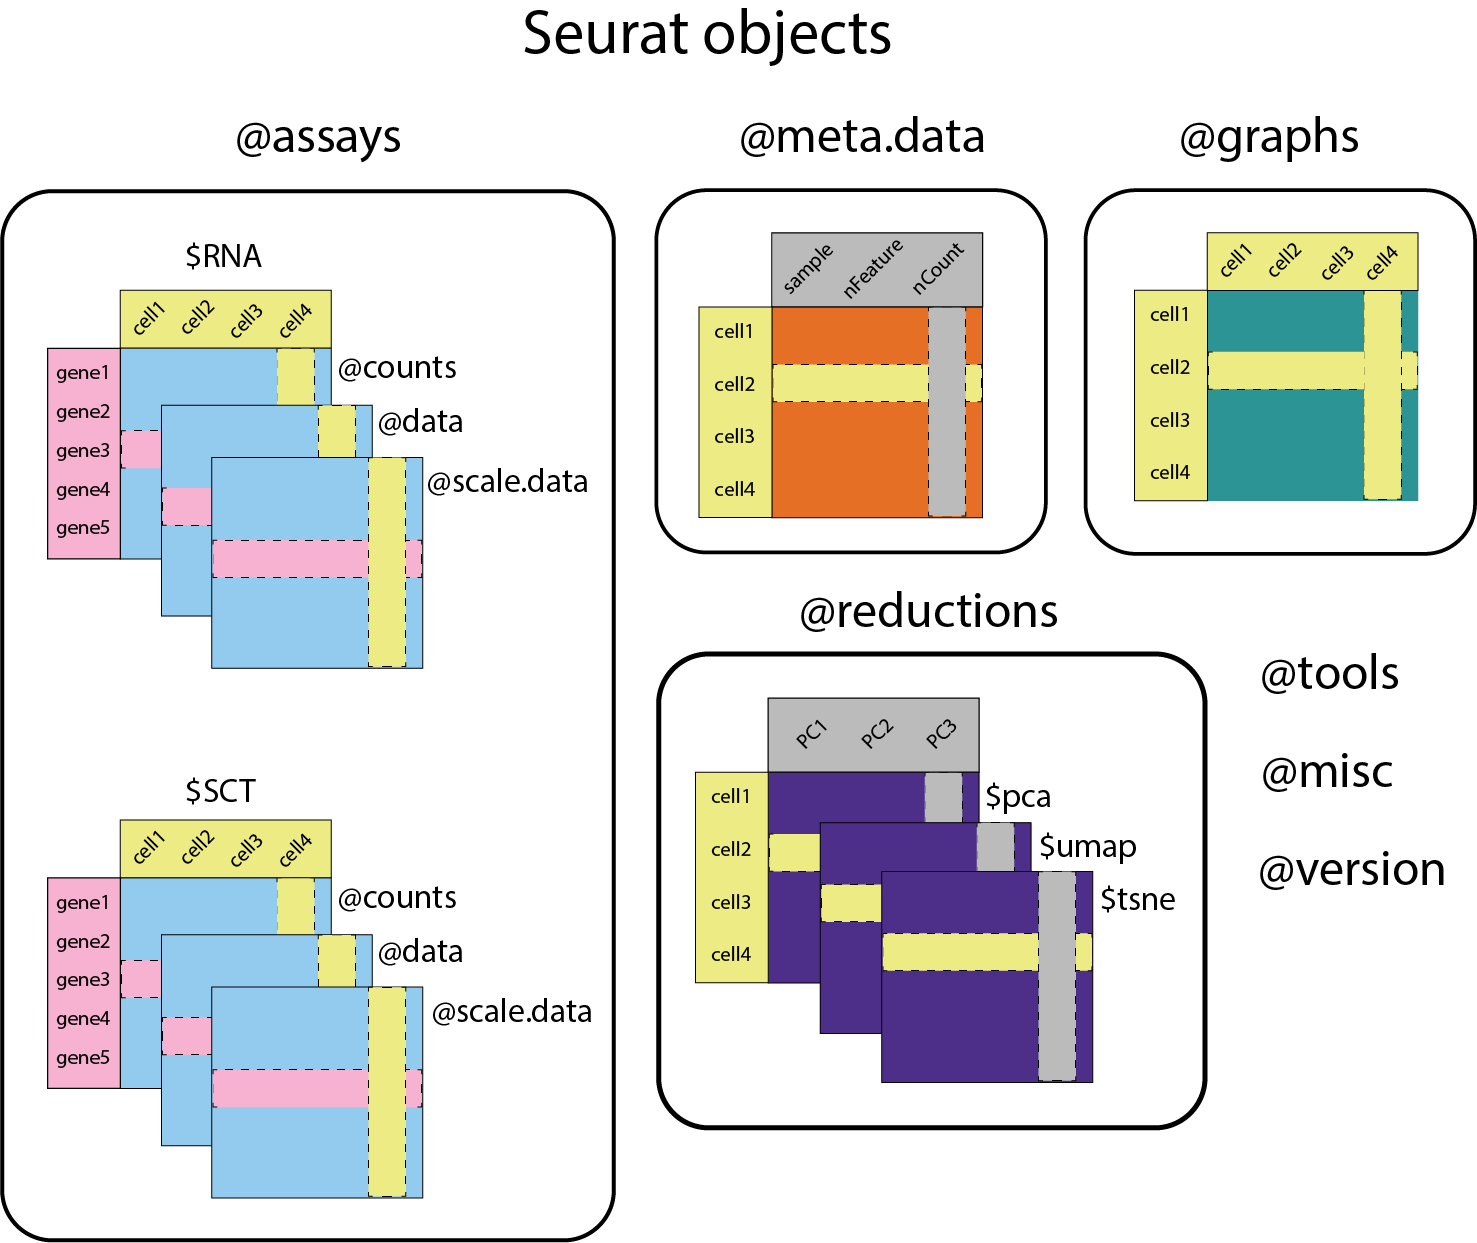
\includegraphics[width=4.89583in,height=4.16667in]{image/seurat_object.png}

}

\caption{Schematic of a Seurat object}

\end{figure}%

\begin{itemize}
\tightlist
\item
  Each Seurat object is composed of different components:

  \begin{itemize}
  \tightlist
  \item
    \textbf{\texttt{assays}} is a list of all the assays in the object.

    \begin{itemize}
    \item
      Defaults to \texttt{RNA} assay, but you can add others (like
      \texttt{SCT} for normalized counts, shown in the figure above,
      could also be antibody-derived tags, etc.).
    \item
      You can see all assays using \texttt{Assays(ifnb)}, see which
      assay is the currently active assay by looking in the
      \texttt{active.assay} slot (\texttt{ifnb@active.assay}) and switch
      between them using the \texttt{DefaultAssay()} function
      (\texttt{DefaultAssay(ifnb)\ \textless{}-\ \textquotesingle{}RNA\textquotesingle{}}).
    \item
      Each assay will store multiple transformations of the data in
      different \texttt{slots} (or \texttt{layers} in Seurat v5) -- in
      the case of \texttt{RNA} data these slots are:

      \begin{itemize}
      \tightlist
      \item
        \texttt{@counts} contains the raw counts.
      \item
        \texttt{@data} contains the normalized counts.
      \item
        \texttt{@scale.data} contains the scaled data for dimensional
        reduction.
      \end{itemize}
    \item
      The \texttt{slots} (Seurat v4) or \texttt{layers} (Seurat v5)
      store the data as a sparse matrix where the rows are gene and the
      columns are cells.
    \item
      In Seurat v4, you could access the raw counts like
      this:\texttt{GetAssayData(ifnb,\ assay=\textquotesingle{}RNA\textquotesingle{},\ slot=\textquotesingle{}counts\textquotesingle{})}.
      This will still work in Seurat v5, but you'll get a warning
      message. In Seurat v5 it is intended that you access the counts
      using the \texttt{LayerData} function, like this:
      \texttt{LayerData(ifnb,\ assay=\textquotesingle{}RNA\textquotesingle{},\ layer=\textquotesingle{}counts\textquotesingle{})}
    \item
      In either version of Seurat
      \texttt{ifnb{[}{[}\textquotesingle{}RNA\textquotesingle{}{]}{]}\$counts}
      will also work.
    \end{itemize}
  \item
    \textbf{\texttt{meta.data}} is a matrix of all the cell-level
    metadata.

    \begin{itemize}
    \tightlist
    \item
      This will include information about which condition, timepoint,
      batch, etc. a for a given cell.
    \item
      It also includes metrics that will be relevant for QC, like
      \texttt{nCount\_RNA} and \texttt{nFeature\_RNA}

      \begin{itemize}
      \tightlist
      \item
        \texttt{nCount\_RNA} is the total number of molecules (UMIs)
        detected within a cell.
      \item
        \texttt{nFeature\_RNA} is the total number of genes detected
        within a cell.
      \end{itemize}
    \item
      Once you have completed clustering, you'll also see information
      about which cluster each cell has been assigned to.
    \item
      The different categories or columns in the \texttt{meta.data} are
      also called \texttt{Idents} in Seurat.
    \item
      You can see the current \texttt{Ident} in the
      \texttt{active.ident} slot (\texttt{ifnb@active.ident}) and switch
      between them using the \texttt{Idents()} function (this will
      probably be important for running differential expression
      testing).
    \item
      You can use \texttt{table(Idents(ifnb))} for a quick summary of
      the number of cells in each grouping.
    \end{itemize}
  \item
    \textbf{\texttt{graphs}} is a list of the nearest neighbor graphs.

    \begin{itemize}
    \tightlist
    \item
      The objects stored in \texttt{graphs} are cell x cell matrices
      containing the neighborhood overlap (Jaccard index) between every
      cell and its nearest neighbors.
    \end{itemize}
  \item
    \textbf{\texttt{reductions}} is a list of \texttt{DimReduc} objects.
  \item
    \textbf{\texttt{version}} contains information about which version
    of Seurat was used to make the object.
  \item
    There are other optional slots, including \textbf{\texttt{tools}}
    and \textbf{\texttt{misc}} that can be populated by specific
    analysis tools (\texttt{tools}) or users can store their own
    additional information (\texttt{misc}).
  \end{itemize}
\end{itemize}

\section{Importing data and interacting with Seurat
objects}\label{importing-data-and-interacting-with-seurat-objects}

We are using the \texttt{SeuratData} package for some test data, which
is already installed in this container.

\begin{Shaded}
\begin{Highlighting}[]
\NormalTok{SeuratData}\SpecialCharTok{::}\FunctionTok{AvailableData}\NormalTok{() }\SpecialCharTok{\%\textgreater{}\%} \FunctionTok{data.frame}\NormalTok{() }\SpecialCharTok{\%\textgreater{}\%}\NormalTok{ dplyr}\SpecialCharTok{::}\FunctionTok{filter}\NormalTok{(Installed }\SpecialCharTok{==} \StringTok{\textquotesingle{}TRUE\textquotesingle{}}\NormalTok{)}
\end{Highlighting}
\end{Shaded}

\begin{verbatim}
                  Dataset Version                           Summary species
ifnb.SeuratData      ifnb   3.1.0 IFNB-Stimulated and Control PBMCs   human
pbmc3k.SeuratData  pbmc3k   3.1.4        3k PBMCs from 10X Genomics   human
                  system ncells   tech seurat default.dataset disk.datasets
ifnb.SeuratData     PBMC  13999 10x v1   <NA>             raw          <NA>
pbmc3k.SeuratData   PBMC   2700 10x v1  3.1.4             raw          <NA>
                  other.datasets notes Installed InstalledVersion
ifnb.SeuratData        processed  <NA>      TRUE            3.1.0
pbmc3k.SeuratData   pbmc3k.final  <NA>      TRUE            3.1.4
\end{verbatim}

It is more likely that you are using Seurat with your own data -- you
can use the functions \texttt{Read10X} or \texttt{Read10X\_h5} to import
data. \texttt{Read10X\_h5} works with H5 files -- ``Hierarchical Data
Format (HDF5 or H5). H5 is a binary format that can compress and access
data much more efficiently than text formats such as MEX, which is
especially useful when dealing with large datasets.''
https://support.10xgenomics.com/single-cell-gene-expression/software/pipelines/latest/advanced/h5\_matrices.
You can also use \texttt{Read10X} and give a path to a folder that
contains your matrix, features, and barcode tsv files. After you have
read in the 10X data, use it as the input to the
\texttt{CreateSeuratObject} function.

We can look at the Seurat object we've loaded from SeuratData:

\begin{Shaded}
\begin{Highlighting}[]
\NormalTok{?ifnb}
\NormalTok{ifnb}
\end{Highlighting}
\end{Shaded}

\begin{verbatim}
An object of class Seurat 
14053 features across 13999 samples within 1 assay 
Active assay: RNA (14053 features, 0 variable features)
 2 layers present: counts, data
\end{verbatim}

The \texttt{ifnb} dataset is 14,000 IFNB-Stimulated and Control PBMCs
(peripheral blood mononuclear cells).

\begin{Shaded}
\begin{Highlighting}[]
\NormalTok{?pbmc3k}
\NormalTok{pbmc3k}
\end{Highlighting}
\end{Shaded}

\begin{verbatim}
An object of class Seurat 
13714 features across 2700 samples within 1 assay 
Active assay: RNA (13714 features, 0 variable features)
 2 layers present: counts, data
\end{verbatim}

The \texttt{pbmc3k} dataset is 2,700 PBMCs (peripheral blood mononuclear
cells).

We can also see that Seurat v5 assays store data in layers. These layers
can store raw, un-normalized counts (layer=`counts'), normalized data
(layer=`data') or z-scored/variance-stabilized data
(layer=`scale.data'). What assays and meta.data are available?

\begin{Shaded}
\begin{Highlighting}[]
\NormalTok{ifnb}\SpecialCharTok{@}\NormalTok{assays}
\end{Highlighting}
\end{Shaded}

\begin{verbatim}
$RNA
Assay data with 14053 features for 13999 cells
First 10 features:
 AL627309.1, RP11-206L10.2, LINC00115, NOC2L, KLHL17, PLEKHN1, HES4,
ISG15, AGRN, C1orf159 
\end{verbatim}

\begin{Shaded}
\begin{Highlighting}[]
\FunctionTok{head}\NormalTok{(ifnb}\SpecialCharTok{@}\NormalTok{meta.data)}
\end{Highlighting}
\end{Shaded}

\begin{verbatim}
                  orig.ident nCount_RNA nFeature_RNA stim seurat_annotations
AAACATACATTTCC.1 IMMUNE_CTRL       3017          877 CTRL          CD14 Mono
AAACATACCAGAAA.1 IMMUNE_CTRL       2481          713 CTRL          CD14 Mono
AAACATACCTCGCT.1 IMMUNE_CTRL       3420          850 CTRL          CD14 Mono
AAACATACCTGGTA.1 IMMUNE_CTRL       3156         1109 CTRL                pDC
AAACATACGATGAA.1 IMMUNE_CTRL       1868          634 CTRL       CD4 Memory T
AAACATACGGCATT.1 IMMUNE_CTRL       1581          557 CTRL          CD14 Mono
\end{verbatim}

We have an \texttt{RNA} assay, and metadata contains information about
which experimental condition the cell came from (\texttt{orig.ident} and
\texttt{stim}), the number of genes (\texttt{nFeature\_RNA}) and
molecules (\texttt{nCount\_RNA}) in each cell. This particular object
also comes pre-annotated (\texttt{seurat\_annotations}).

If we look at the unique values in \texttt{orig.ident}, we see that
there's \texttt{IMMUNE\_CTRL} and \texttt{IMMUNE\_STIM} samples in one
Seurat object.

\begin{Shaded}
\begin{Highlighting}[]
\FunctionTok{table}\NormalTok{(ifnb}\SpecialCharTok{@}\NormalTok{meta.data}\SpecialCharTok{$}\NormalTok{orig.ident)}
\end{Highlighting}
\end{Shaded}

\begin{verbatim}

IMMUNE_CTRL IMMUNE_STIM 
       6548        7451 
\end{verbatim}

\begin{Shaded}
\begin{Highlighting}[]
\NormalTok{pbmc3k}\SpecialCharTok{@}\NormalTok{assays}
\end{Highlighting}
\end{Shaded}

\begin{verbatim}
$RNA
Assay data with 13714 features for 2700 cells
First 10 features:
 AL627309.1, AP006222.2, RP11-206L10.2, RP11-206L10.9, LINC00115, NOC2L,
KLHL17, PLEKHN1, RP11-54O7.17, HES4 
\end{verbatim}

\begin{Shaded}
\begin{Highlighting}[]
\FunctionTok{head}\NormalTok{(pbmc3k}\SpecialCharTok{@}\NormalTok{meta.data)}
\end{Highlighting}
\end{Shaded}

\begin{verbatim}
               orig.ident nCount_RNA nFeature_RNA seurat_annotations
AAACATACAACCAC     pbmc3k       2419          779       Memory CD4 T
AAACATTGAGCTAC     pbmc3k       4903         1352                  B
AAACATTGATCAGC     pbmc3k       3147         1129       Memory CD4 T
AAACCGTGCTTCCG     pbmc3k       2639          960         CD14+ Mono
AAACCGTGTATGCG     pbmc3k        980          521                 NK
AAACGCACTGGTAC     pbmc3k       2163          781       Memory CD4 T
\end{verbatim}

\begin{Shaded}
\begin{Highlighting}[]
\FunctionTok{table}\NormalTok{(pbmc3k}\SpecialCharTok{@}\NormalTok{meta.data}\SpecialCharTok{$}\NormalTok{orig.ident)}
\end{Highlighting}
\end{Shaded}

\begin{verbatim}

pbmc3k 
  2700 
\end{verbatim}

If we look at the unique values in \texttt{orig.ident} for the
\texttt{pbmc3k} object, we see that there's only \texttt{pbmc3k}
samples.

\section{Data QC}\label{data-qc}

First, lets subset our datasets so they are smaller and easier to work
with for this workshop.

\begin{Shaded}
\begin{Highlighting}[]
\NormalTok{pbmc3k }\OtherTok{\textless{}{-}} \FunctionTok{subset}\NormalTok{(pbmc3k, }\AttributeTok{downsample =} \DecValTok{500}\NormalTok{)}
\NormalTok{ifnb }\OtherTok{\textless{}{-}} \FunctionTok{subset}\NormalTok{(ifnb, }\AttributeTok{downsample =} \DecValTok{500}\NormalTok{)}
\end{Highlighting}
\end{Shaded}

\begin{itemize}
\tightlist
\item
  For now, let's merge the datasets to make our QC and filtering a bit
  smoother.
\item
  \texttt{merge()} merges the raw count matrices of two Seurat objects
  and creates a new Seurat object with the resulting combined raw count
  matrix.
\item
  To explicitly specify the original object any particular cell came
  from, you can set the \texttt{add.cell.ids} parameter with an c(x, y)
  vector, which will prepend the given identifier to the beginning of
  each cell name.
\item
  The original project ID will remain stored in object meta data under
  \texttt{orig.ident}.
\end{itemize}

\begin{Shaded}
\begin{Highlighting}[]
\NormalTok{all\_data }\OtherTok{\textless{}{-}} \FunctionTok{merge}\NormalTok{(}\AttributeTok{x =}\NormalTok{ ifnb, }\AttributeTok{y =}\NormalTok{ pbmc3k, }\AttributeTok{add.cell.ids =} \FunctionTok{c}\NormalTok{(}\StringTok{"ifnb"}\NormalTok{, }\StringTok{"pbmc3k"}\NormalTok{), }\AttributeTok{project =} \StringTok{\textquotesingle{}pbmc\textquotesingle{}}\NormalTok{)}
\end{Highlighting}
\end{Shaded}

\begin{itemize}
\tightlist
\item
  We care about the percentage of reads that map to the mitochondrial
  genome because high mitochondrial reads in a cell can indicate that
  the cells are low-quality or dying cells
\item
  The mitochondrial QC metrics are calcualted with the
  \texttt{PercentageFeatureSet()} function, which calculates the
  percentage of counts originating from a set of features
\item
  We use the set of all genes starting with MT- as a set of
  mitochondrial genes -- the format of the mt sequences will vary
  depending on which organism/genome is used\ldots(might be `mt-' for
  example).
\end{itemize}

\begin{Shaded}
\begin{Highlighting}[]
\FunctionTok{rownames}\NormalTok{(all\_data) }\SpecialCharTok{\%\textgreater{}\%} \FunctionTok{grep}\NormalTok{(}\AttributeTok{pattern =} \StringTok{\textquotesingle{}\^{}mt{-}\textquotesingle{}}\NormalTok{, }\AttributeTok{ignore.case =} \ConstantTok{TRUE}\NormalTok{, }\AttributeTok{value =} \ConstantTok{TRUE}\NormalTok{)}
\end{Highlighting}
\end{Shaded}

\begin{verbatim}
 [1] "MT-ND1"  "MT-ND2"  "MT-CO1"  "MT-CO2"  "MT-ATP8" "MT-ATP6" "MT-CO3" 
 [8] "MT-ND3"  "MT-ND4L" "MT-ND4"  "MT-ND5"  "MT-ND6"  "MT-CYB" 
\end{verbatim}

\begin{itemize}
\tightlist
\item
  Then add the percent mitochondrial reads to the metadata:
\end{itemize}

\begin{Shaded}
\begin{Highlighting}[]
\NormalTok{all\_data[[}\StringTok{"percent.mt"}\NormalTok{]] }\OtherTok{\textless{}{-}} \FunctionTok{PercentageFeatureSet}\NormalTok{(all\_data, }\AttributeTok{pattern =} \StringTok{"\^{}MT{-}"}\NormalTok{)}
\end{Highlighting}
\end{Shaded}

\begin{itemize}
\tightlist
\item
  Before we plot, we can set the order of the object idents to whatever
  order we'd like:
\end{itemize}

\begin{Shaded}
\begin{Highlighting}[]
\FunctionTok{Idents}\NormalTok{(all\_data) }\OtherTok{\textless{}{-}} \StringTok{\textquotesingle{}orig.ident\textquotesingle{}}
\FunctionTok{levels}\NormalTok{(all\_data) }\OtherTok{\textless{}{-}} \FunctionTok{c}\NormalTok{(}\StringTok{"pbmc3k"}\NormalTok{, }\StringTok{"IMMUNE\_CTRL"}\NormalTok{, }\StringTok{"IMMUNE\_STIM"}\NormalTok{)}
\end{Highlighting}
\end{Shaded}

\begin{itemize}
\tightlist
\item
  We can also look at plots showing the distribution of the
  \texttt{percent.mt}, \texttt{nFeature\_RNA} and \texttt{nCount\_RNA}
\item
  \texttt{nFeature\_RNA} is the number of genes
\item
  \texttt{nCount\_RNA} is the number of UMIs (unique molecules -- like
  counts)
\end{itemize}

\begin{Shaded}
\begin{Highlighting}[]
\FunctionTok{VlnPlot}\NormalTok{(all\_data, }\AttributeTok{features =} \StringTok{"nFeature\_RNA"}\NormalTok{)}
\end{Highlighting}
\end{Shaded}

\pandocbounded{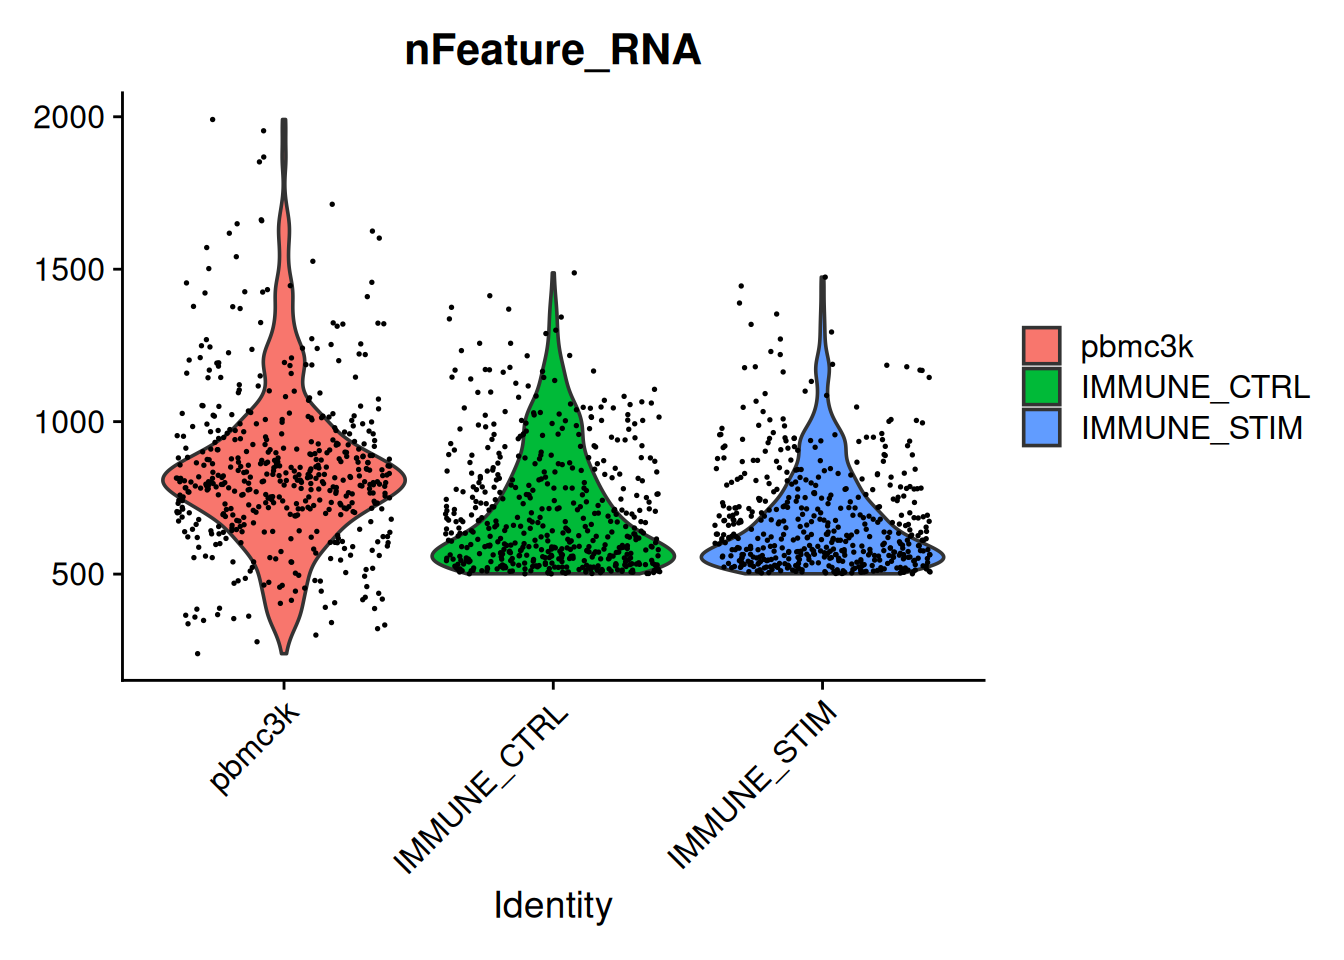
\includegraphics[keepaspectratio]{Intro_files/figure-pdf/unnamed-chunk-15-1.pdf}}

\begin{Shaded}
\begin{Highlighting}[]
\FunctionTok{VlnPlot}\NormalTok{(all\_data, }\AttributeTok{features =} \StringTok{"nCount\_RNA"}\NormalTok{)}
\end{Highlighting}
\end{Shaded}

\pandocbounded{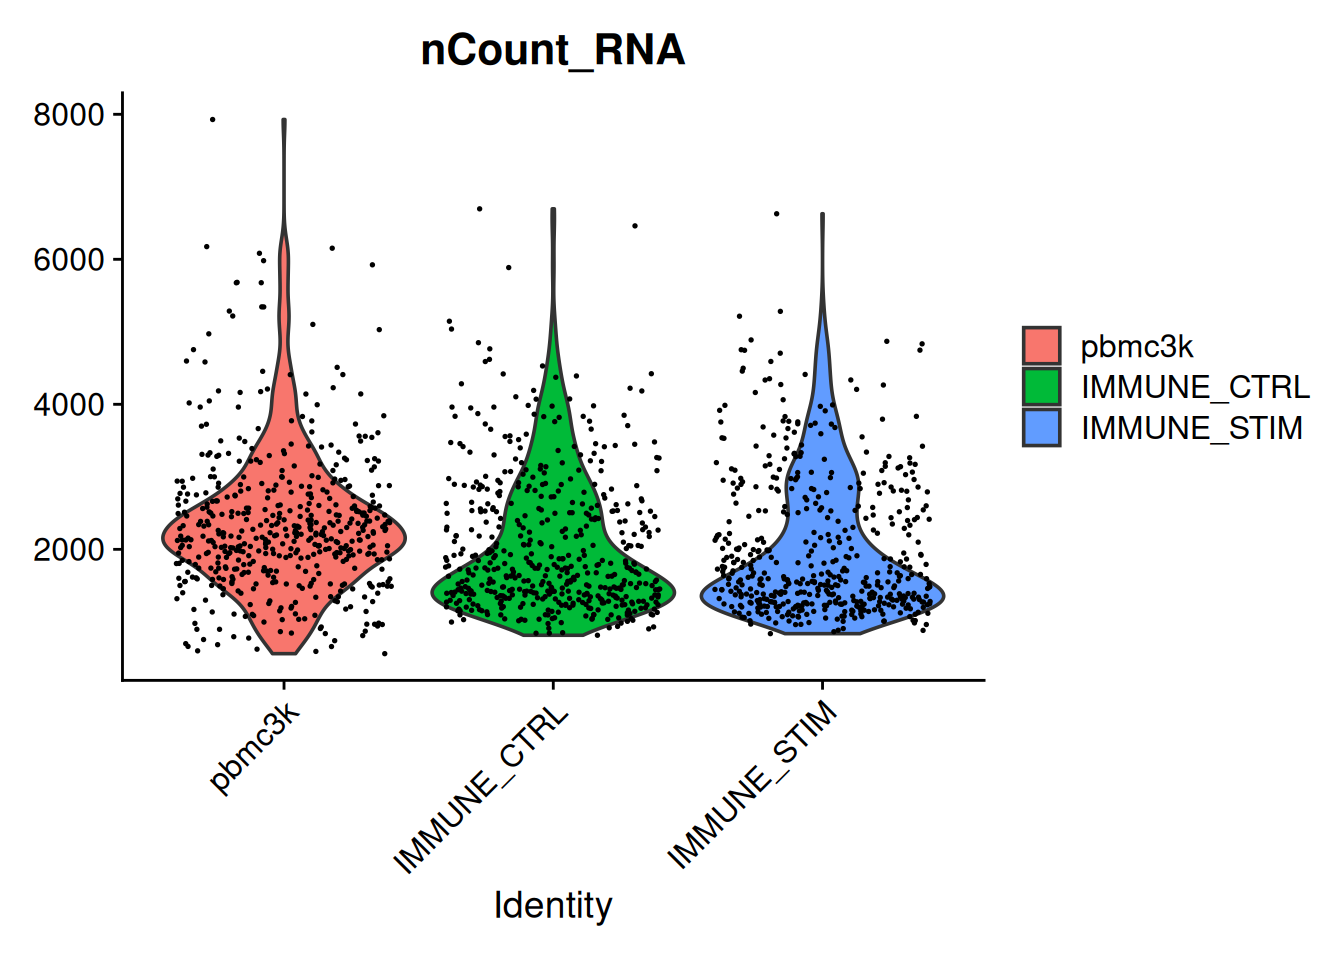
\includegraphics[keepaspectratio]{Intro_files/figure-pdf/unnamed-chunk-16-1.pdf}}

\begin{Shaded}
\begin{Highlighting}[]
\FunctionTok{VlnPlot}\NormalTok{(all\_data, }\AttributeTok{features=}\StringTok{"percent.mt"}\NormalTok{)}
\end{Highlighting}
\end{Shaded}

\pandocbounded{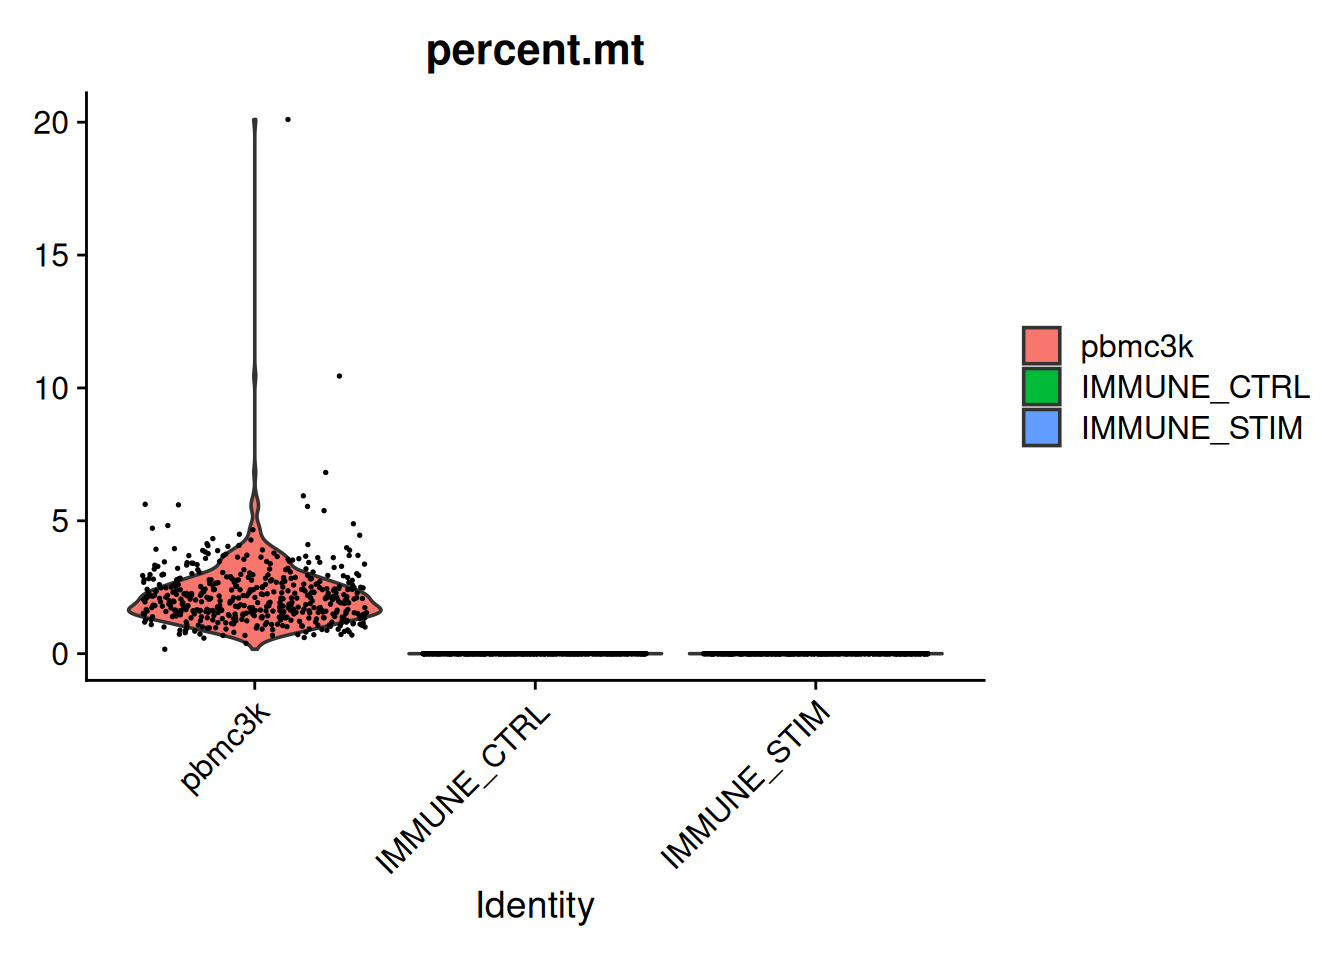
\includegraphics[keepaspectratio]{Intro_files/figure-pdf/unnamed-chunk-17-1.pdf}}

\begin{Shaded}
\begin{Highlighting}[]
\FunctionTok{FeatureScatter}\NormalTok{(all\_data, }\AttributeTok{feature1 =} \StringTok{"nCount\_RNA"}\NormalTok{, }\AttributeTok{feature2 =} \StringTok{"nFeature\_RNA"}\NormalTok{)}
\end{Highlighting}
\end{Shaded}

\pandocbounded{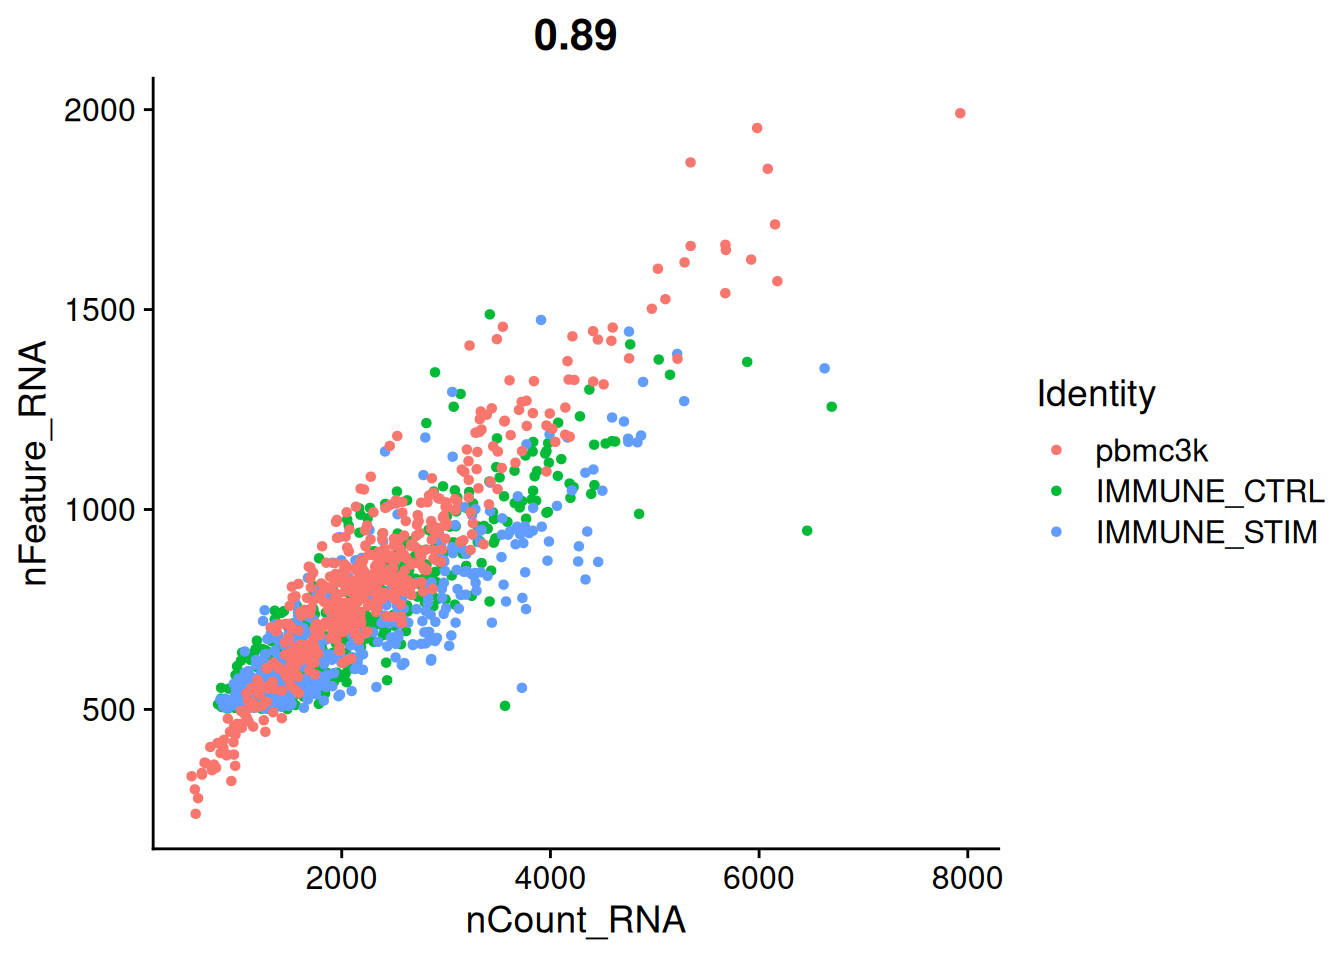
\includegraphics[keepaspectratio]{Intro_files/figure-pdf/unnamed-chunk-18-1.pdf}}

\begin{Shaded}
\begin{Highlighting}[]
\FunctionTok{FeatureScatter}\NormalTok{(all\_data, }\AttributeTok{feature1 =} \StringTok{"nCount\_RNA"}\NormalTok{, }\AttributeTok{feature2 =} \StringTok{"percent.mt"}\NormalTok{)}
\end{Highlighting}
\end{Shaded}

\pandocbounded{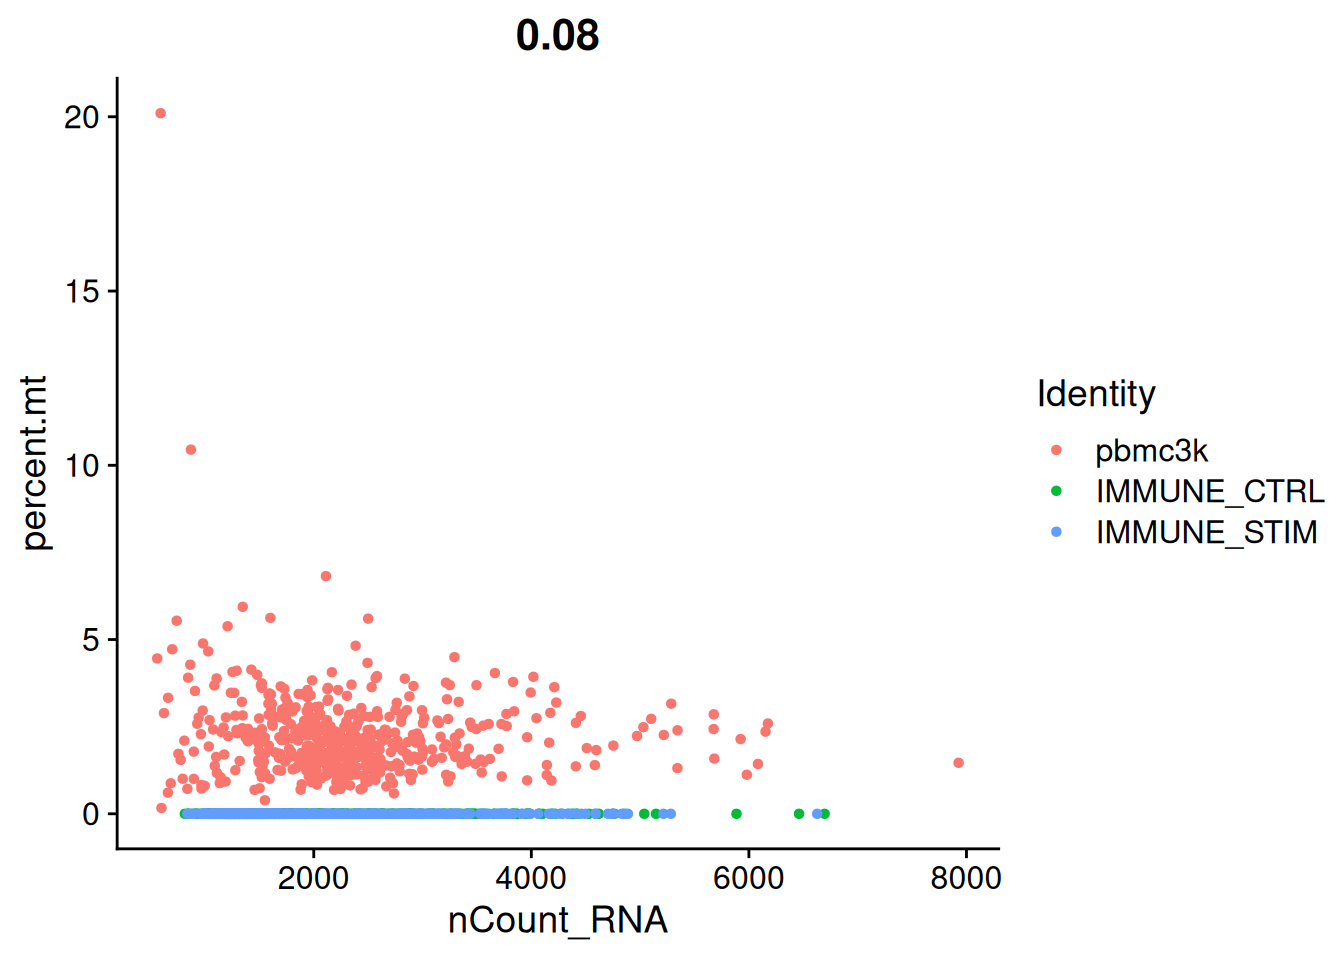
\includegraphics[keepaspectratio]{Intro_files/figure-pdf/unnamed-chunk-19-1.pdf}}

\begin{Shaded}
\begin{Highlighting}[]
\FunctionTok{FeatureScatter}\NormalTok{(all\_data, }\AttributeTok{feature1 =} \StringTok{"nFeature\_RNA"}\NormalTok{, }\AttributeTok{feature2 =} \StringTok{"percent.mt"}\NormalTok{)}
\end{Highlighting}
\end{Shaded}

\pandocbounded{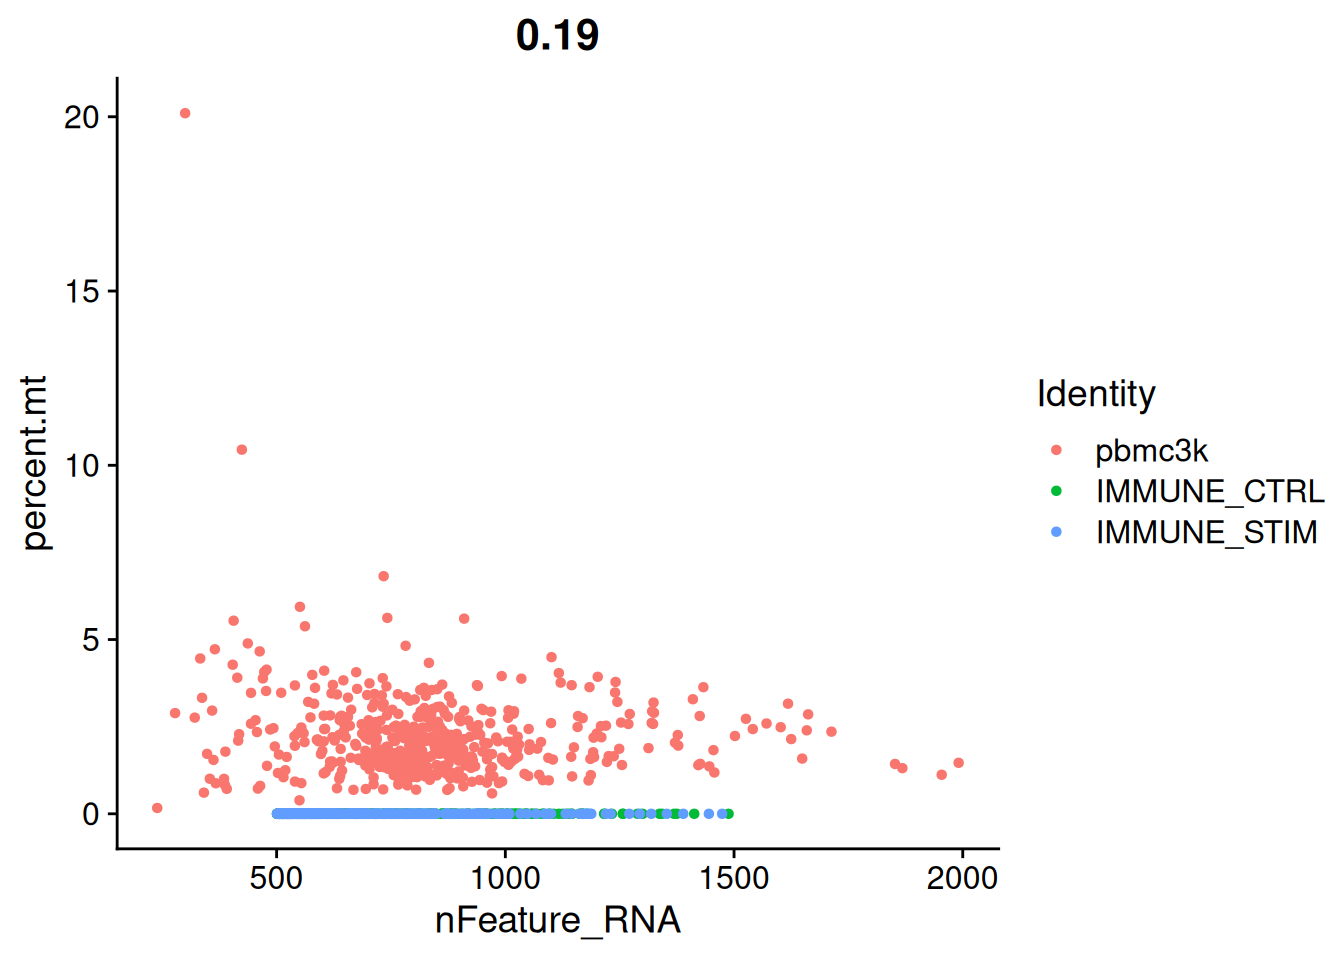
\includegraphics[keepaspectratio]{Intro_files/figure-pdf/unnamed-chunk-20-1.pdf}}

You can also just use ggplot to make your own custom visualizations of
the information in the metadata. We make a separate matrix called
\texttt{qc\_data} and sorting it based on the \texttt{percent.mt}
column. Then we make our own ggplot and specify that the x and y axes
should be \texttt{nCount\_RNA} and \texttt{nFeature\_RNA} and that the
points should be colored based on \texttt{percent.mt}. Then, use
\texttt{scale\_color\_gradientn} to specify how the points should be
colored, specifying that the limit should be between 0 and 10 and that
we should \texttt{squish} anything that is out of bounds (effectively
making our limits 0 and \textgreater10).

\begin{Shaded}
\begin{Highlighting}[]
\NormalTok{qc\_data }\OtherTok{\textless{}{-}}\NormalTok{ all\_data}\SpecialCharTok{@}\NormalTok{meta.data[}\FunctionTok{c}\NormalTok{(}\StringTok{\textquotesingle{}orig.ident\textquotesingle{}}\NormalTok{,}\StringTok{\textquotesingle{}nCount\_RNA\textquotesingle{}}\NormalTok{,}\StringTok{\textquotesingle{}nFeature\_RNA\textquotesingle{}}\NormalTok{,}\StringTok{\textquotesingle{}percent.mt\textquotesingle{}}\NormalTok{)] }\SpecialCharTok{\%\textgreater{}\%} \FunctionTok{arrange}\NormalTok{(percent.mt)}

\NormalTok{ggplot2}\SpecialCharTok{::}\FunctionTok{ggplot}\NormalTok{(qc\_data, ggplot2}\SpecialCharTok{::}\FunctionTok{aes}\NormalTok{(}\AttributeTok{x =}\NormalTok{ nCount\_RNA, }\AttributeTok{y =}\NormalTok{ nFeature\_RNA, }\AttributeTok{color =}\NormalTok{ percent.mt)) }\SpecialCharTok{+} 
\NormalTok{  ggplot2}\SpecialCharTok{::}\FunctionTok{geom\_point}\NormalTok{() }\SpecialCharTok{+} 
\NormalTok{ ggplot2}\SpecialCharTok{::} \FunctionTok{scale\_color\_gradientn}\NormalTok{(}\AttributeTok{colors =} \FunctionTok{rev}\NormalTok{(}\FunctionTok{brewer.pal}\NormalTok{(}\DecValTok{5}\NormalTok{, }\StringTok{"Spectral"}\NormalTok{)), }\AttributeTok{limits =} \FunctionTok{c}\NormalTok{(}\DecValTok{0}\NormalTok{,}\DecValTok{10}\NormalTok{), }\AttributeTok{oob =}\NormalTok{ (scales}\SpecialCharTok{::}\NormalTok{squish)) }\SpecialCharTok{+}
\NormalTok{  ggplot2}\SpecialCharTok{::}\FunctionTok{facet\_wrap}\NormalTok{(}\SpecialCharTok{\textasciitilde{}}\NormalTok{orig.ident) }\SpecialCharTok{+} 
\NormalTok{  ggplot2}\SpecialCharTok{::}\FunctionTok{theme\_bw}\NormalTok{()}
\end{Highlighting}
\end{Shaded}

\pandocbounded{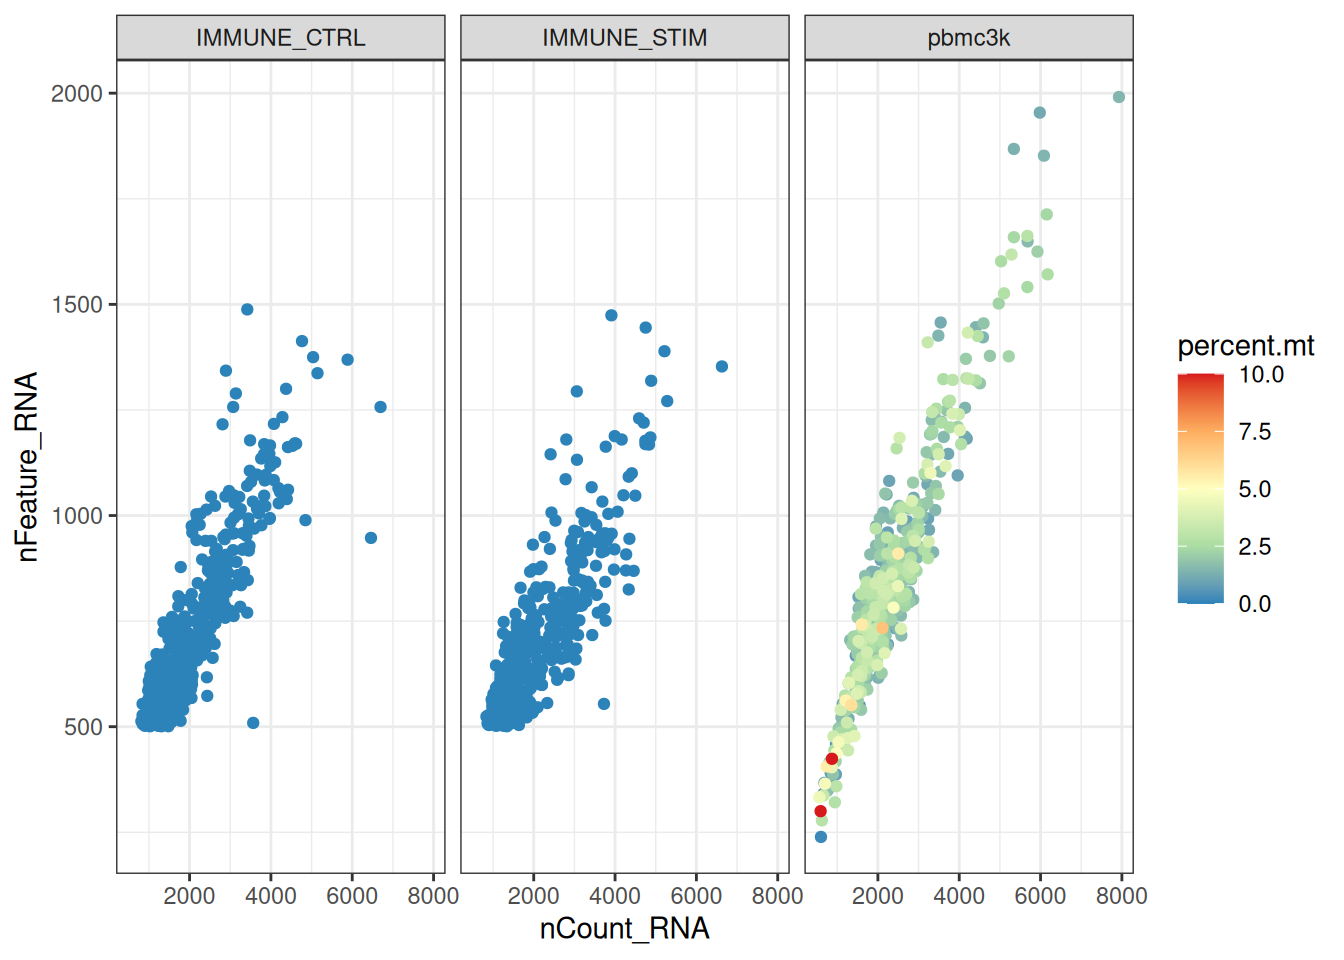
\includegraphics[keepaspectratio]{Intro_files/figure-pdf/unnamed-chunk-21-1.pdf}}

\begin{itemize}
\tightlist
\item
  Low quality cells or empty droplets might have very few genes
  (\texttt{nFeatures})
\item
  Dead or dying cells will also have high mitochondrial reads
  (\texttt{percent.mt})
\item
  Doublets or multiplets will have high gene counts (\texttt{nFeatures})
\item
  The total number of molecules (\texttt{nCount}) detected in a cell
  corresponds with the number of genes (\texttt{nFeatures})
\item
  Most of the cells have less than 2000 genes and less than 7000 or so
  UMIs.
\item
  Very low mitochondrial counts from the \texttt{ifnb} data and the
  nFeature\_RNA scatter plots look strange -- perhaps this dataset was
  pre-filtered before being packaged into SeuratData.
\item
  In the \texttt{pbmc3k} data, we can see groups of cells with high
  mitochondrial counts, low UMI counts, and lower numbers of genes.
\item
  Our goal in QC filtering is to retain as much useful information as we
  can, while removing doublets, empty droplets, and dead cells.
\item
  We will pick some thresholds for filtering based off of what we see in
  our data, keeping in mind that if you are doing this with your own
  data, your plots will probably look a bit different.
\end{itemize}

\begin{tcolorbox}[enhanced jigsaw, breakable, toprule=.15mm, colframe=quarto-callout-important-color-frame, opacitybacktitle=0.6, coltitle=black, title=\textcolor{quarto-callout-important-color}{\faExclamation}\hspace{0.5em}{Important}, rightrule=.15mm, toptitle=1mm, arc=.35mm, bottomtitle=1mm, leftrule=.75mm, colbacktitle=quarto-callout-important-color!10!white, titlerule=0mm, bottomrule=.15mm, opacityback=0, left=2mm, colback=white]

We don't get into it in this workshop, but an additional QC
consideration is ambient RNA. Look at this document from 10x for more
information:
https://www.10xgenomics.com/analysis-guides/introduction-to-ambient-rna-correction

\end{tcolorbox}

\section{Data Filtering}\label{data-filtering}

\begin{itemize}
\tightlist
\item
  Let's filter our data using \texttt{subset}, we'll keep cells that
  have between 500 and 7000 nFeature\_RNA (genes) and less than 5\%
  mitochondrial reads.
\end{itemize}

\begin{Shaded}
\begin{Highlighting}[]
\NormalTok{all\_data\_sub }\OtherTok{\textless{}{-}} \FunctionTok{subset}\NormalTok{(all\_data, }\AttributeTok{subset =}\NormalTok{ nFeature\_RNA }\SpecialCharTok{\textgreater{}} \DecValTok{500} \SpecialCharTok{\&}\NormalTok{ nFeature\_RNA }\SpecialCharTok{\textless{}} \DecValTok{7000} \SpecialCharTok{\&}\NormalTok{ percent.mt }\SpecialCharTok{\textless{}} \DecValTok{5}\NormalTok{)}
\end{Highlighting}
\end{Shaded}

\begin{itemize}
\tightlist
\item
  You can re-examine your QC plots after filtering if you'd like:
\end{itemize}

\begin{Shaded}
\begin{Highlighting}[]
\NormalTok{qc\_data\_sub }\OtherTok{\textless{}{-}}\NormalTok{ all\_data\_sub}\SpecialCharTok{@}\NormalTok{meta.data[}\FunctionTok{c}\NormalTok{(}\StringTok{\textquotesingle{}orig.ident\textquotesingle{}}\NormalTok{,}\StringTok{\textquotesingle{}nCount\_RNA\textquotesingle{}}\NormalTok{,}\StringTok{\textquotesingle{}nFeature\_RNA\textquotesingle{}}\NormalTok{,}\StringTok{\textquotesingle{}percent.mt\textquotesingle{}}\NormalTok{)] }\SpecialCharTok{\%\textgreater{}\%} \FunctionTok{arrange}\NormalTok{(percent.mt)}

\NormalTok{ggplot2}\SpecialCharTok{::}\FunctionTok{ggplot}\NormalTok{(qc\_data\_sub,ggplot2}\SpecialCharTok{::} \FunctionTok{aes}\NormalTok{(}\AttributeTok{x =}\NormalTok{ nCount\_RNA, }\AttributeTok{y =}\NormalTok{ nFeature\_RNA, }\AttributeTok{color =}\NormalTok{ percent.mt)) }\SpecialCharTok{+} 
\NormalTok{  ggplot2}\SpecialCharTok{::}\FunctionTok{geom\_point}\NormalTok{() }\SpecialCharTok{+} 
\NormalTok{  ggplot2}\SpecialCharTok{::}\FunctionTok{scale\_color\_gradientn}\NormalTok{(}\AttributeTok{colors =} \FunctionTok{rev}\NormalTok{(}\FunctionTok{brewer.pal}\NormalTok{(}\DecValTok{5}\NormalTok{, }\StringTok{"Spectral"}\NormalTok{)), }\AttributeTok{limits =} \FunctionTok{c}\NormalTok{(}\DecValTok{0}\NormalTok{,}\DecValTok{10}\NormalTok{), }\AttributeTok{oob =}\NormalTok{ (scales}\SpecialCharTok{::}\NormalTok{squish)) }\SpecialCharTok{+}
\NormalTok{  ggplot2}\SpecialCharTok{::}\FunctionTok{facet\_wrap}\NormalTok{(}\SpecialCharTok{\textasciitilde{}}\NormalTok{orig.ident) }\SpecialCharTok{+} 
\NormalTok{  ggplot2}\SpecialCharTok{::}\FunctionTok{theme\_bw}\NormalTok{()}
\end{Highlighting}
\end{Shaded}

\pandocbounded{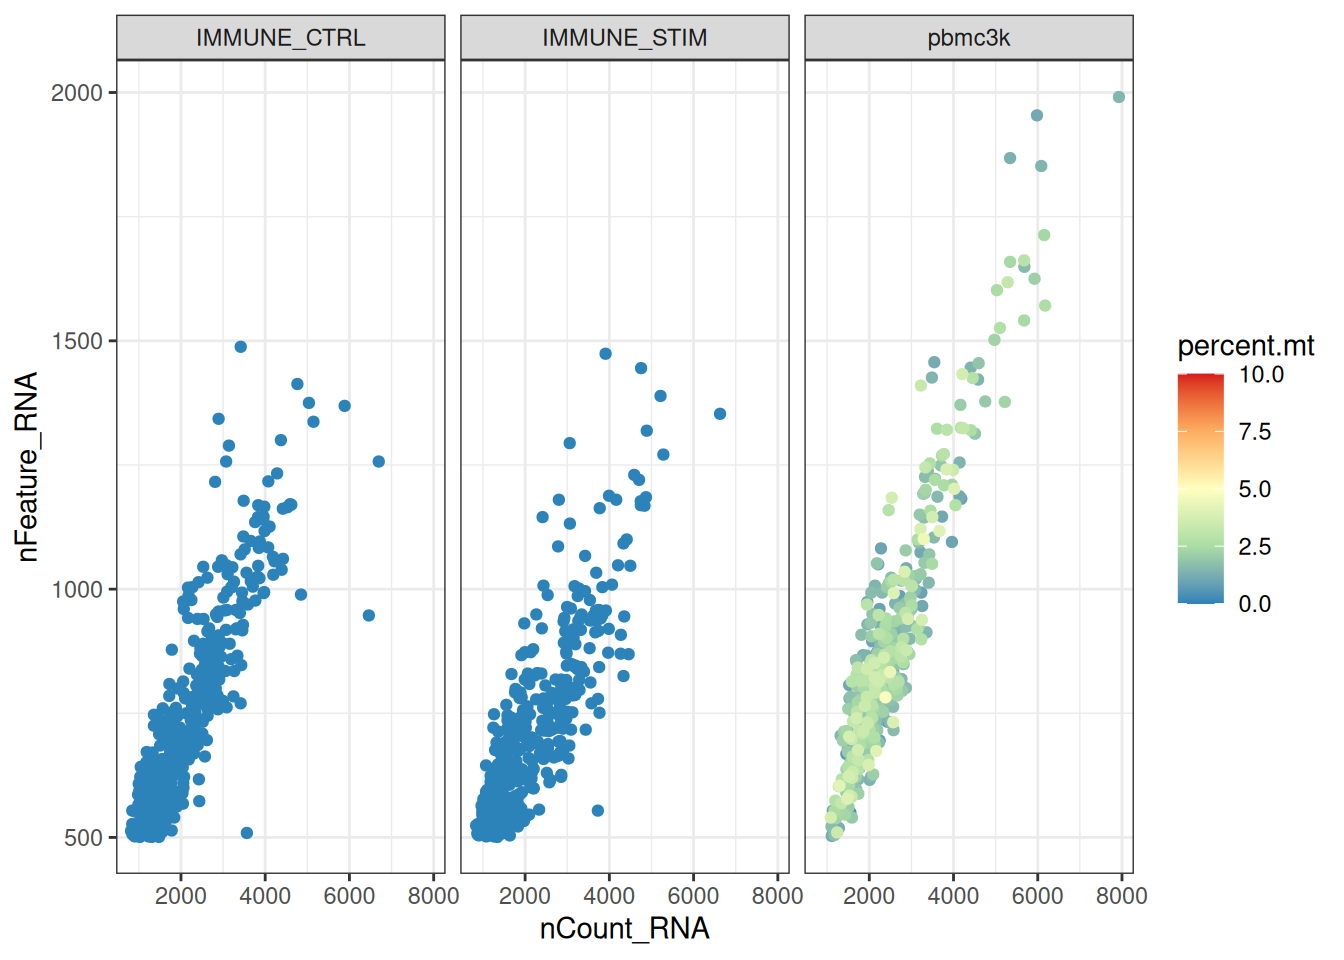
\includegraphics[keepaspectratio]{Intro_files/figure-pdf/unnamed-chunk-23-1.pdf}}

\begin{itemize}
\tightlist
\item
  We can also take a look at how many cells we lost from filtering:
\end{itemize}

\begin{Shaded}
\begin{Highlighting}[]
\FunctionTok{table}\NormalTok{(all\_data}\SpecialCharTok{@}\NormalTok{meta.data}\SpecialCharTok{$}\NormalTok{orig.ident)}
\end{Highlighting}
\end{Shaded}

\begin{verbatim}

IMMUNE_CTRL IMMUNE_STIM      pbmc3k 
        500         500         500 
\end{verbatim}

\begin{Shaded}
\begin{Highlighting}[]
\FunctionTok{table}\NormalTok{(all\_data\_sub}\SpecialCharTok{@}\NormalTok{meta.data}\SpecialCharTok{$}\NormalTok{orig.ident)}
\end{Highlighting}
\end{Shaded}

\begin{verbatim}

IMMUNE_CTRL IMMUNE_STIM      pbmc3k 
        500         500         456 
\end{verbatim}

\section{Normalization}\label{normalization}

\subsection{Theory}\label{theory}

scRNAseq data is normalized so that we can mitigate technical effects
while preserving the biological signal in the data -- we should be able
to find the biological signal in cells irrespective of how deeply we
sequenced the cell. The theory behind SCTransform
(https://genomebiology.biomedcentral.com/articles/10.1186/s13059-019-1874-1)
is very similar to the generalized linear models (GLMs) used in bulk
RNAseq analysis packages like DESeq2 and edgeR. In DESeq2 a negative
binomial model is fitted to the counts and the mean and dispersion
(roughly speaking how variable the observed count will be from the mean
count) estimates from that model are used as the test statistics for
comparison between group and the same idea applies with SCTransform.
SCTransform also pools information across genes with similar abundances
in order to address the higher sparsity of single cell data.

Below is a side-by-side comparison of sctransform with NormalizeData,
FindVariableFeatures and ScaleData on the PBMC3k data:

\begin{figure}[H]

{\centering \pandocbounded{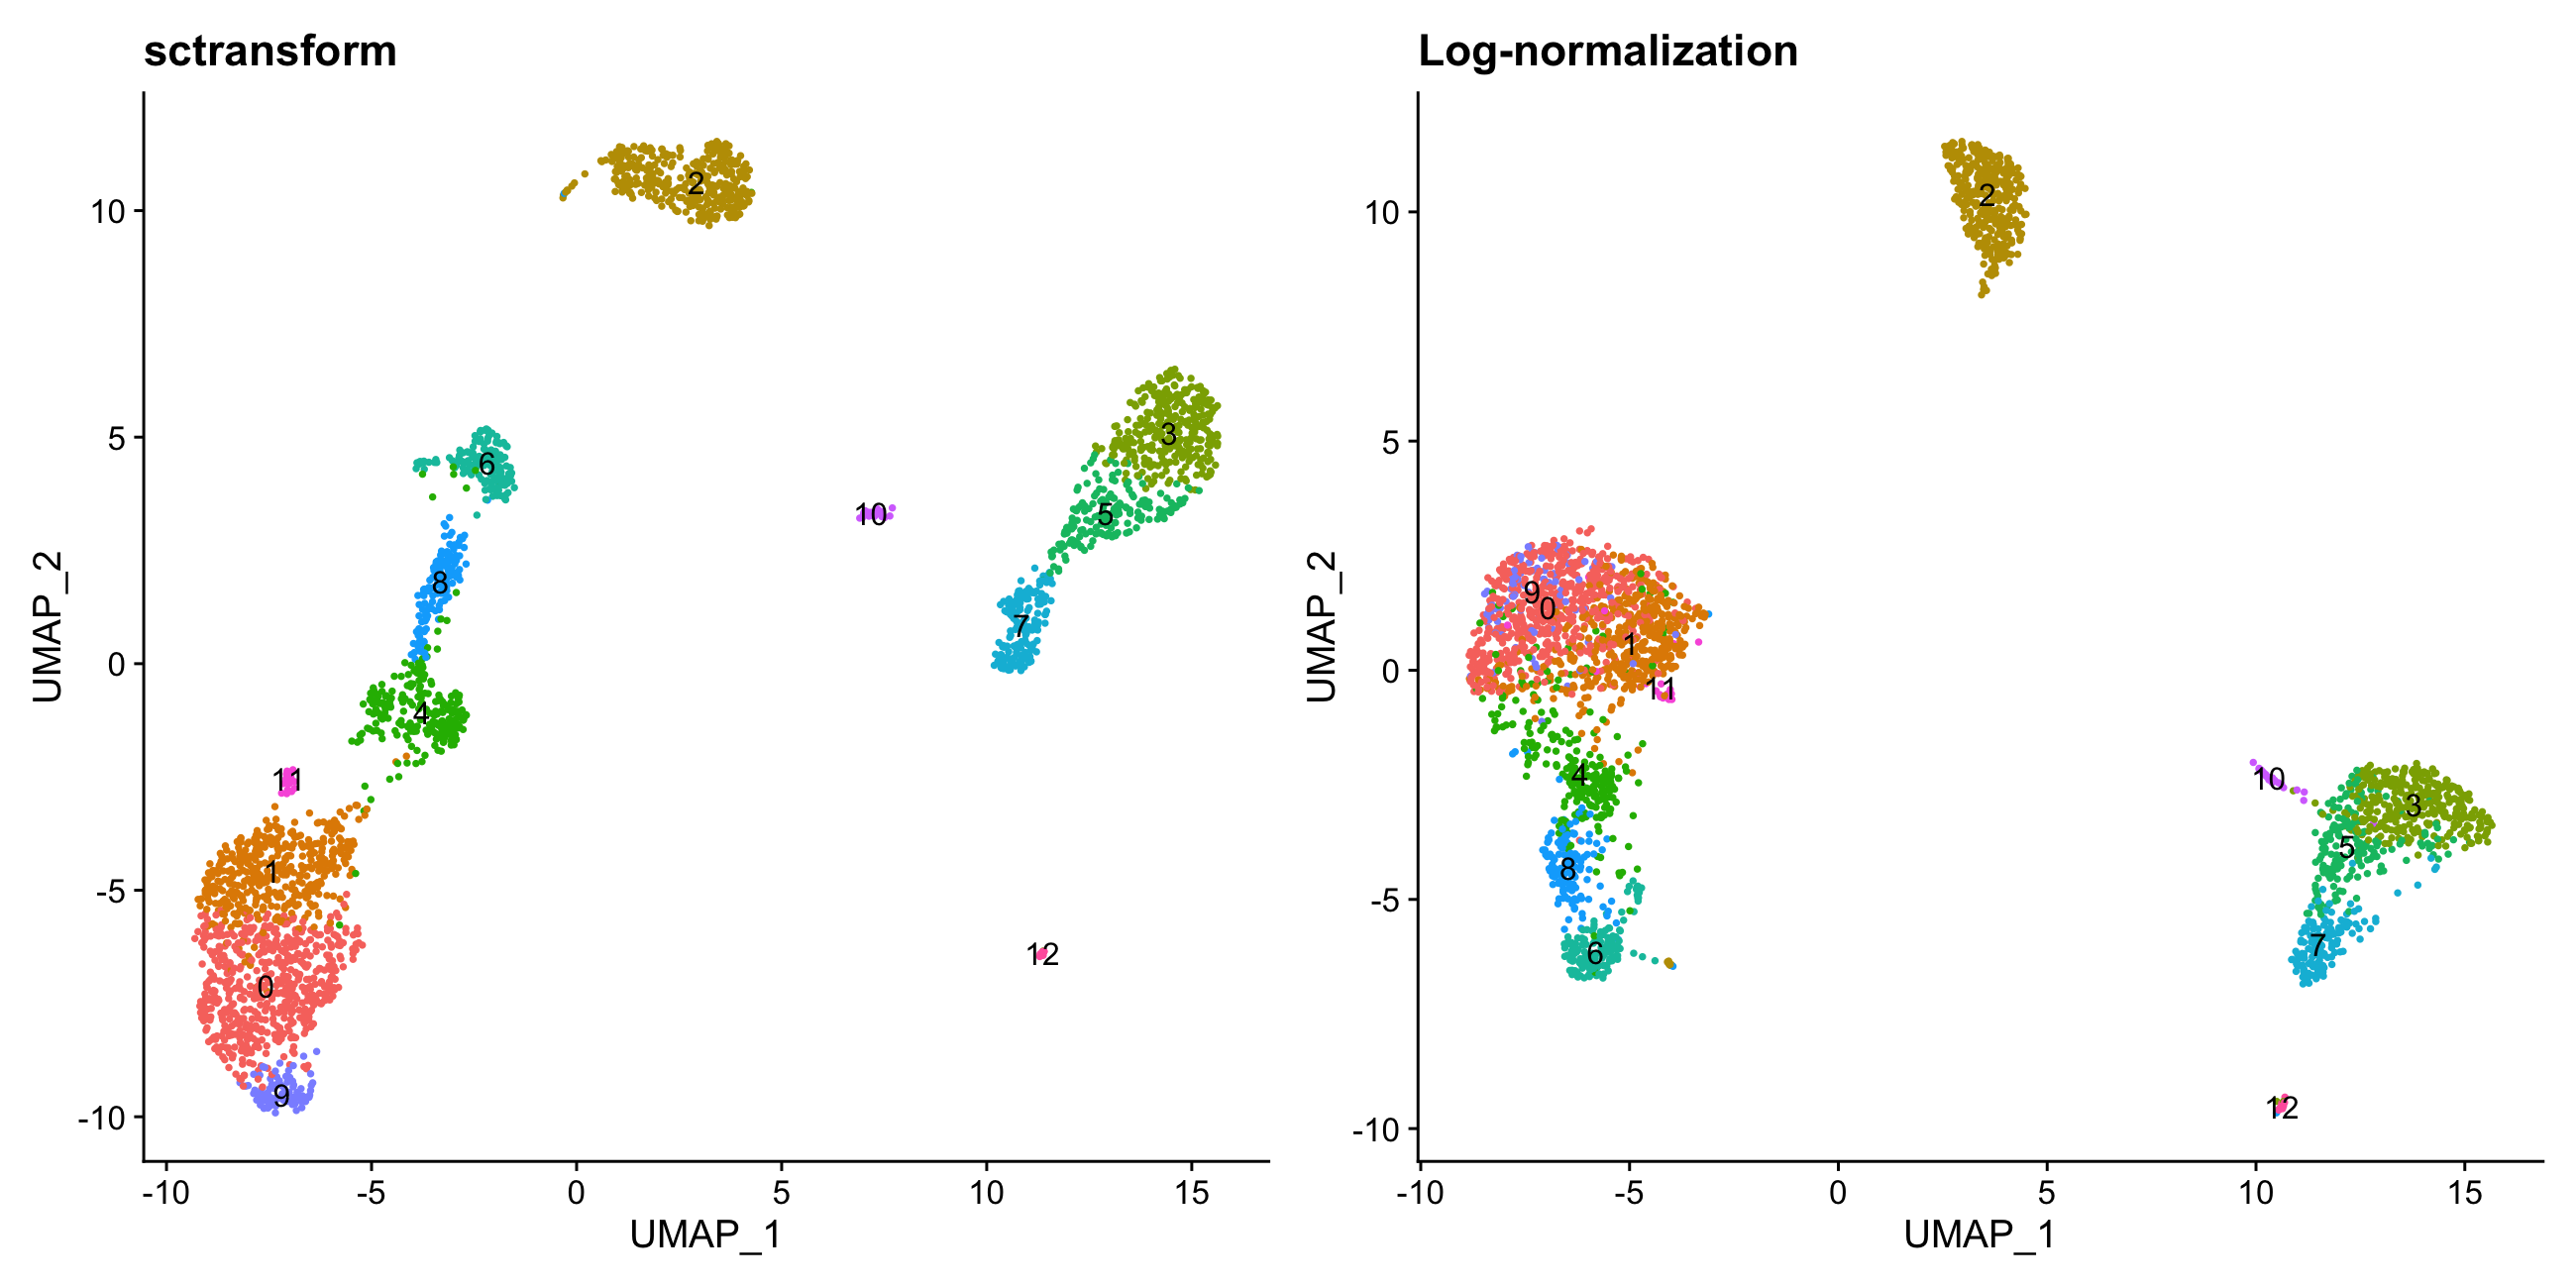
\includegraphics[keepaspectratio]{image/sctransform_vs_regular.png}}

}

\caption{sct}

\end{figure}%

We also like this figure from the SCTransform paper, which shows how
SCTransform (`Pearson Residuals') and the standard log-transformation
approach (`Log-normalization') helps alleviate variance in your data
from sequencing depth alone :

\begin{figure}[H]

{\centering \pandocbounded{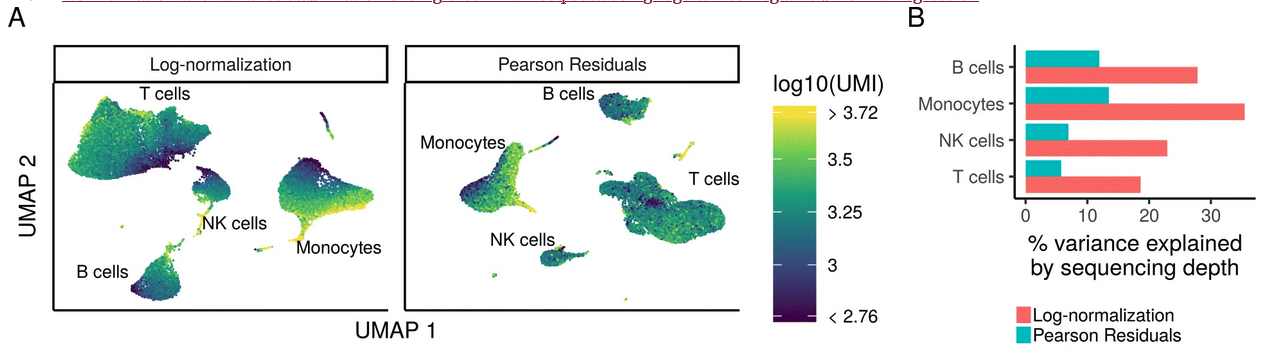
\includegraphics[keepaspectratio]{image/sct_fig6.png}}

}

\caption{sct\_fig6}

\end{figure}%

\subsection{When should you not use
SCTransform?}\label{when-should-you-not-use-sctransform}

The paper states:

\texttt{As\ our\ workflow\ leverages\ all\ genes\ (or\ a\ random\ subset)\ for\ the\ initial\ regularization,\ we\ make\ an\ implicit\ assumption\ that\ the\ majority\ of\ genes\ in\ the\ dataset\ do\ not\ exhibit\ significant\ biological\ variation...this\ assumption\ may\ be\ overly\ simplistic\ when\ performing\ scRNA-seq\ on\ a\ highly\ heterogeneous\ sample,\ we\ did\ not\ observe\ adverse\ affects\ when\ applying\ our\ model\ to\ human\ PBMC\ data,\ or\ any\ of\ the\ other\ datasets\ we\ examined.}

SCTransform might not work well if your data is highly heterogeneous and
you expect that a high proportion of genes will exhibit significant
biological variation across your samples. In this case, we would
recommend the more standard workflow of \texttt{NormalizeData},
\texttt{FindVariableFeatures}, and \texttt{ScaleData}.

\subsection{SCTransform versions}\label{sctransform-versions}

Seurat v5 runs SCTransform v2
(https://satijalab.org/seurat/archive/v4.3/sctransform\_v2\_vignette) by
default, while Seurat v4 runs SCTransform v1 by default. SCTransform v2
``improves speed and memory consumption, the stability of parameter
estimates, the identification of variable features, and the the ability
to perform downstream differential expression analyses.'' This means you
might get different results if you run Seurat v5 and re-normalize data
that you have previously processed with Seurat v4. If you want to change
from the default veresion of SCTransform, you can add the argument
\texttt{vst.flavor\ =\ "v1"} (or \texttt{vst.flavor\ =\ "v2"}))

\subsection{Running SCTransform}\label{running-sctransform}

We will normalize using SCTransform and you might get see a warning that
says `iteration limit reached' when you run the function. This warning
can be ignored (https://github.com/satijalab/sctransform/issues/25)
because the parameter estimation generating this warning is regularized
later anyway. You can use the \texttt{vars.to.regress} argument to
regress out nuisance variables (like cell cycle, batch effects, or
\texttt{percent.mt}). By default SCTransform will only return data for
variable genes in the scale data slot -- adding the
\texttt{return.only.var.genes\ =\ FALSE} argument to the function call
to turn this option off
(https://github.com/satijalab/seurat/issues/3553). In previous versions
of Seurat, you would have to split your object into a list of Seurat
objects based on the \texttt{orig.ident} and then run
\texttt{SCTransform} on the list, which is not necessary in Seurat v5 --
but we do have to split the layers by their \texttt{orig.ident}:

\begin{Shaded}
\begin{Highlighting}[]
\NormalTok{all\_data\_sub[[}\StringTok{"RNA"}\NormalTok{]] }\OtherTok{\textless{}{-}} \FunctionTok{split}\NormalTok{(all\_data\_sub[[}\StringTok{"RNA"}\NormalTok{]], }\AttributeTok{f =}\NormalTok{ all\_data\_sub}\SpecialCharTok{$}\NormalTok{orig.ident)}
\end{Highlighting}
\end{Shaded}

\begin{verbatim}
Warning: Input is a v3 assay and `split()` only works for v5 assays; converting
* to a v5 assay
\end{verbatim}

\begin{verbatim}
Warning: Assay RNA changing from Assay to Assay5
\end{verbatim}

\begin{Shaded}
\begin{Highlighting}[]
\NormalTok{start.time }\OtherTok{\textless{}{-}} \FunctionTok{Sys.time}\NormalTok{()}
\NormalTok{all\_data\_sub }\OtherTok{\textless{}{-}} \FunctionTok{SCTransform}\NormalTok{(all\_data\_sub, }\AttributeTok{vars.to.regress =} \StringTok{"percent.mt"}\NormalTok{, }\AttributeTok{verbose =} \ConstantTok{FALSE}\NormalTok{)}
\NormalTok{end.time }\OtherTok{\textless{}{-}} \FunctionTok{Sys.time}\NormalTok{()}
\NormalTok{end.time }\SpecialCharTok{{-}}\NormalTok{ start.time}
\end{Highlighting}
\end{Shaded}

\begin{verbatim}
Time difference of 18.41443 secs
\end{verbatim}

Then run PCA

\begin{Shaded}
\begin{Highlighting}[]
\NormalTok{all\_data\_sub }\OtherTok{\textless{}{-}} \FunctionTok{RunPCA}\NormalTok{(all\_data\_sub)}
\end{Highlighting}
\end{Shaded}

\begin{verbatim}
PC_ 1 
Positive:  FTL, TIMP1, FTH1, LYZ, TYROBP, CST3, FCER1G, S100A9, SOD2, LGALS1 
       S100A8, APOBEC3A, S100A4, HLA-DRA, LGALS3, FCN1, TYMP, S100A11, IFITM3, SAT1 
       AIF1, S100A6, ANXA5, CD63, CTSB, HLA-DRB1, LST1, PSAP, IL8, NPC2 
Negative:  RPL3, RPS6, RPS18, LTB, RPL13, RPL13A, RPL21, RPS27A, RPS3A, RPS3 
       RPS27, RPL34, GIMAP7, RPL7, MALAT1, CD3D, RPS15A, CCR7, RPS4X, RPS2 
       LDHB, RPS14, RPS12, RPL9, RPL32, RPL10, RPL23A, RPL31, RPSA, RPS5 
PC_ 2 
Positive:  NKG7, CCL5, GZMB, GNLY, PRF1, CST7, GZMA, CTSW, FGFBP2, GZMH 
       CCL4, CLIC3, FCGR3A, APOBEC3G, KLRD1, CD247, GZMM, B2M, CHST12, HOPX 
       UBB, C1orf21, AKR1C3, APMAP, IGFBP7, CD7, RARRES3, ACTB, SRGN, C12orf75 
Negative:  RPL13, RPS18, RPL13A, RPL32, HLA-DRA, RPS2, RPL10, RPL3, RPS12, RPL34 
       LTB, RPS6, RPS14, RPS4X, RPL18A, RPS3A, RPS5, RPL11, CD74, RPL7 
       RPL10A, RPS15A, CCR7, RPS27, RPL19, RPS13, RPS8, RPL21, RPL12, RPS27A 
PC_ 3 
Positive:  CD3D, GIMAP7, IL32, CD7, SOD2, CD3E, GIMAP5, CD2, CCL5, IL7R 
       LCK, GIMAP4, LDHB, RPL34, RARRES3, TIMP1, ANXA1, CTSL, CD3G, APOBEC3A 
       RPS14, LAT, RPS12, ZFP36L2, NKG7, RPL3, PABPC1, IFI27, RPS3, LTB 
Negative:  CD74, HLA-DRA, HLA-DQA1, HLA-DPB1, HLA-DRB1, HLA-DPA1, HLA-DQB1, CD79A, HERPUD1, MS4A1 
       HLA-DMA, CD83, HLA-DRB5, IRF8, CD79B, PMAIP1, REL, HSP90AB1, BIRC3, SYNGR2 
       HSPD1, CST3, CCR7, PRMT1, ID3, RAN, RPL22L1, LYZ, CYCS, BLNK 
PC_ 4 
Positive:  S100A9, S100A8, LYZ, FTH1, FTL, FCN1, TYROBP, AIF1, CST3, S100A4 
       S100A6, LST1, LGALS2, COTL1, CACYBP, CD14, OAZ1, SRSF2, LGALS1, NOP58 
       SOD1, GIMAP7, CREM, GPX1, DDIT4, YPEL5, SAT1, TRAT1, SRSF7, CFD 
Negative:  CD74, HLA-DRA, HLA-DPB1, CD79A, HLA-DQA1, HLA-DPA1, NKG7, HLA-DQB1, CCL5, HLA-DRB1 
       CST7, CCL4, CD79B, MS4A1, GNLY, TXN, GZMB, CTSW, TIMP1, SOD2 
       ISG20, GZMA, FGFBP2, PTPRCAP, GZMH, HLA-DMA, B2M, APOBEC3G, PRF1, SLAMF7 
PC_ 5 
Positive:  SOD2, JUNB, HSPB1, HSPA1A, CD69, JUN, SRSF7, NFKBIA, CCL4, APOBEC3A 
       CACYBP, DDIT4, TIMP1, SRSF2, HSPA8, CTSL, HSP90AB1, CLK1, TXN, HSPH1 
       DNAJB1, NOP58, HSP90AA1, CREM, YPEL5, IL1RN, EIF5, DNAJB6, ZFAND2A, TSC22D3 
Negative:  CST3, LYZ, S100A9, S100A8, NKG7, TYROBP, GSTP1, AIF1, GNLY, GZMB 
       LGALS2, LST1, FCN1, S100A6, LGALS1, COTL1, FTH1, CCL5, PYCARD, CEBPD 
       CST7, TMSB4X, ALOX5AP, RPS2, TKT, PRF1, CTSS, RPL3, AP1S2, FGFBP2 
\end{verbatim}

We can make an elbow plot:

\begin{Shaded}
\begin{Highlighting}[]
\FunctionTok{ElbowPlot}\NormalTok{(all\_data\_sub)}
\end{Highlighting}
\end{Shaded}

\pandocbounded{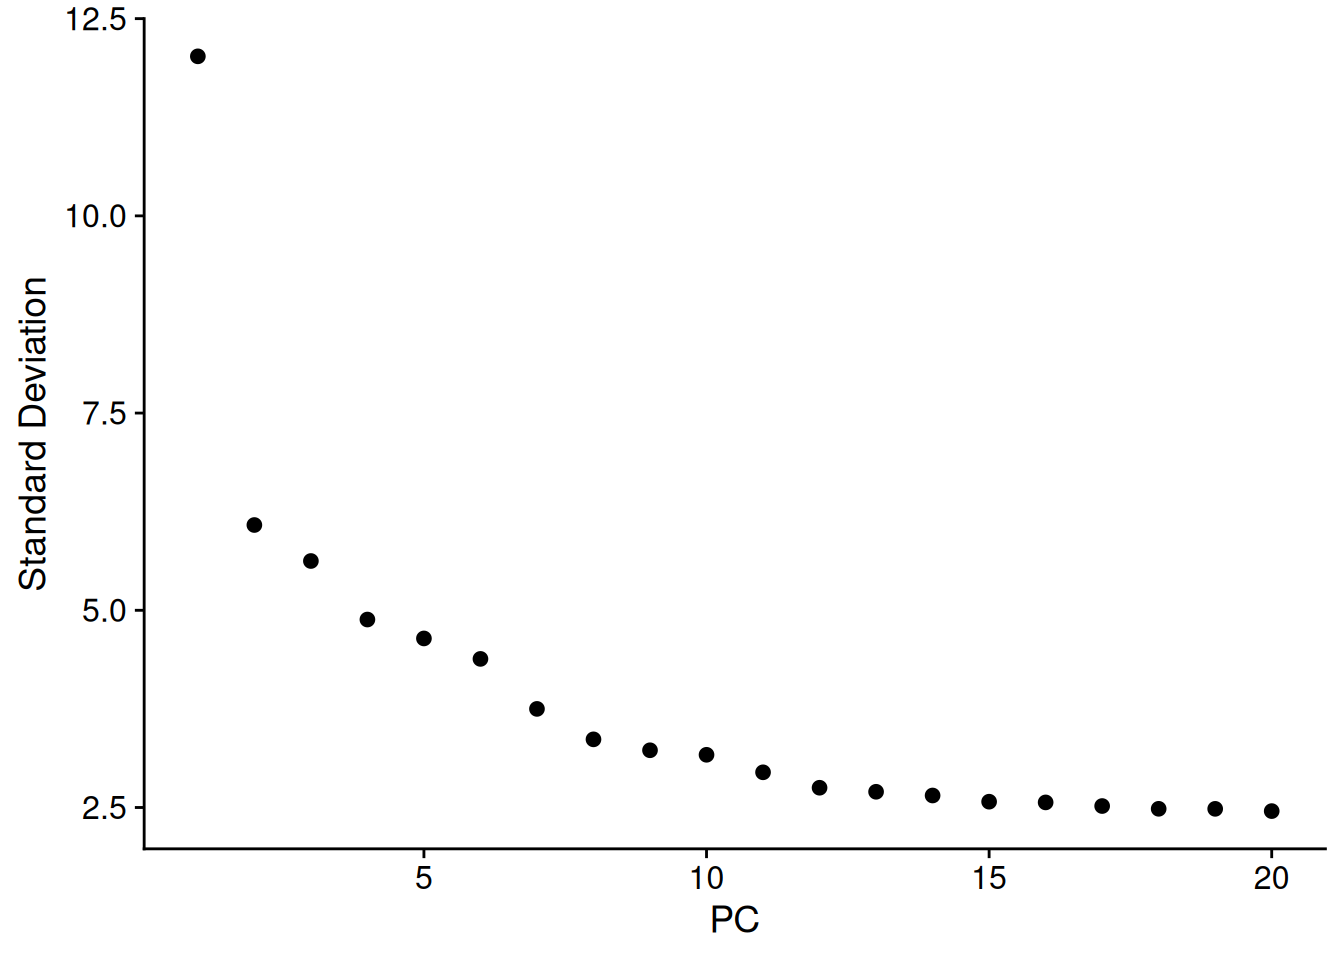
\includegraphics[keepaspectratio]{Intro_files/figure-pdf/unnamed-chunk-28-1.pdf}}

Based on this plot, we get diminishing information returned once we get
above \textasciitilde10-15 PCs. We will use this information when we run
clustering.

\section{Integration}\label{integration}

Integration of single-cell sequencing datasets, for example across
experimental batches, donors, or conditions, is often an important step
in scRNA-seq workflows. Integrative analysis can help to match shared
cell types and states across datasets, which can boost statistical
power, and most importantly, facilitate accurate comparative analysis
across datasets.

While the goal of matching shared cell types across datasets may be
important for many problems, users may also be concerned about which
method to use, or that integration could result in a loss of biological
resolution. In Seurat v5, we introduce more flexible and streamlined
infrastructure to run different integration algorithms with a single
line of code. This makes it easier to explore the results of different
integration methods, and to compare these results to a workflow that
excludes integration steps.

Seurat v5 enables streamlined integrative analysis using the
\texttt{IntegrateLayers} function. The method currently supports four
integration methods by default. Each of these methods performs
integration in low-dimensional space, and returns a dimensional
reduction (i.e.~integrated.rpca) that aims to co-embed shared cell types
across batches (samples). These integration methods can be divided into
two categories:

Anchor-based methods: CCA, RPCA, and JointPCA, which rely on identifying
pairs of cells (anchors) that are mutual nearest neighbors between
datasets

Non-anchor-based methods: Harmony, which uses soft clustering and
iterative correction

\begin{itemize}
\tightlist
\item
  CCA integration (method=CCAIntegration)
\item
  RPCA integration (method=RPCAIntegration)
\item
  Joint PCA integration (method=JointPCAIntegration)
\item
  Harmony (method=HarmonyIntegration)
\end{itemize}

\subsection{Canonical Correlation Analysis (CCA)
Integration}\label{canonical-correlation-analysis-cca-integration}

CCA (Canonical Correlation Analysis) Integration was the first
integration method developed for Seurat. It identifies common sources of
variation between datasets by finding linear combinations of features
with maximum correlation.

\begin{itemize}
\item
  CCA integration:

  \begin{itemize}
  \tightlist
  \item
    Performs canonical correlation analysis between pairs of datasets
  \item
    L2-normalizes the cell embeddings to focus on correlation strength
    rather than magnitude
  \item
    Identifies mutual nearest neighbors (anchors) between datasets in
    the CCA space
  \item
    Uses these anchors to correct the data and align matching cell
    populations
  \end{itemize}
\end{itemize}

By identifying shared sources of variation between datasets, CCA is
well-suited for identifying anchors when cell types are conserved, but
there are very substantial differences in gene expression across
experiments. CCA-based integration therefore enables integrative
analysis when experimental conditions or disease states introduce very
strong expression shifts, or when integrating datasets across modalities
and species. However, CCA-based integration may also lead to
overcorrection, especially when a large proportion of cells are
non-overlapping across datasets.

\subsection{Reciprocal Principal Components Analysis (RPCA)
Integration}\label{reciprocal-principal-components-analysis-rpca-integration}

RPCA (Reciprocal PCA) Integration uses principal component analysis for
integration. Unlike CCA, which finds correlations between datasets, RPCA
projects each dataset onto the other's PCA space.

\begin{itemize}
\item
  RPCA integration:

  \begin{itemize}
  \tightlist
  \item
    Computes PCA on each dataset separately
  \item
    Projects each dataset onto the other's PCA space (reciprocal
    projection)
  \item
    L2-normalizes the cell embeddings
  \item
    Identifies mutual nearest neighbors (anchors) between datasets in
    the projected space
  \item
    Uses these anchors to correct the data and align matching cell
    populations
  \end{itemize}
\end{itemize}

We recommend RPCA during integrative analysis where: A substantial
fraction of cells in one dataset have no matching type in the other,
datasets that originate from the same platform (i.e.~multiple lanes of
10x genomics), or if there are a large number of datasets or cells to
integrate.

\subsection{JointPCA Integration}\label{jointpca-integration}

JointPCA (Joint PCA) Integration first combines all datasets and then
performs PCA on the combined data. This method is simpler but can be
effective when datasets are already somewhat aligned or have minor batch
effects.

\begin{itemize}
\item
  JointPCA integration:

  \begin{itemize}
  \tightlist
  \item
    Merges the datasets into a single matrix
  \item
    Performs PCA on the combined data
  \item
    L2-normalizes the cell embeddings
  \item
    Identifies mutual nearest neighbors (anchors) between original
    datasets in the joint PCA space
  \item
    Uses these anchors to correct the data and align matching cell
    populations
  \end{itemize}
\end{itemize}

JointPCA is often faster than CCA or RPCA but may be less effective for
datasets with substantial differences or batch effects.

\subsection{Harmony Integration}\label{harmony-integration}

Harmony Integration is a different approach developed by the Korsunsky
et al.~team (https://doi.org/10.1038/s41592-019-0619-0). Instead of
using an anchor-based approach, Harmony uses soft clustering and
iterative correction to align datasets.

\begin{itemize}
\item
  Harmony integration:

  \begin{itemize}
  \tightlist
  \item
    Performs PCA on the combined datasets
  \item
    Applies soft clustering to group cells by similarity
  \item
    Iteratively corrects cluster assignments and cell embeddings to
    align datasets
  \item
    Uses ridge regression to minimize the effect of dataset-specific
    variation
  \end{itemize}
\end{itemize}

Harmony is generally faster than anchor-based methods and often performs
well on datasets with complex batch effects.

We will run \texttt{CCAIntegration} (this was the default flavor of
integration in previous versions of Seurat),
\texttt{JointPCAIntegration}, \texttt{HarmonyIntegration}, and
\texttt{RPCAIntegration}. Note that we are specifying that we used
\texttt{SCT} normalization:

\begin{Shaded}
\begin{Highlighting}[]
\NormalTok{start.time }\OtherTok{\textless{}{-}} \FunctionTok{Sys.time}\NormalTok{()}
\NormalTok{all\_data\_sub}\OtherTok{\textless{}{-}} \FunctionTok{IntegrateLayers}\NormalTok{(}
  \AttributeTok{object =}\NormalTok{ all\_data\_sub, }\AttributeTok{method =}\NormalTok{ CCAIntegration,}
  \AttributeTok{orig.reduction =} \StringTok{"pca"}\NormalTok{, }\AttributeTok{new.reduction =} \StringTok{"integrated.cca"}\NormalTok{, }\AttributeTok{normalization.method =} \StringTok{"SCT"}\NormalTok{,}
  \AttributeTok{verbose =} \ConstantTok{FALSE}
\NormalTok{)}
\NormalTok{end.time }\OtherTok{\textless{}{-}} \FunctionTok{Sys.time}\NormalTok{()}
\NormalTok{end.time }\SpecialCharTok{{-}}\NormalTok{ start.time}
\end{Highlighting}
\end{Shaded}

\begin{verbatim}
Time difference of 10.7525 secs
\end{verbatim}

\begin{Shaded}
\begin{Highlighting}[]
\NormalTok{start.time }\OtherTok{\textless{}{-}} \FunctionTok{Sys.time}\NormalTok{()}
\NormalTok{all\_data\_sub }\OtherTok{\textless{}{-}} \FunctionTok{IntegrateLayers}\NormalTok{(}
  \AttributeTok{object =}\NormalTok{ all\_data\_sub, }\AttributeTok{method =}\NormalTok{ JointPCAIntegration,}
  \AttributeTok{orig.reduction =} \StringTok{"pca"}\NormalTok{, }\AttributeTok{new.reduction =} \StringTok{"integrated.jpca"}\NormalTok{, }\AttributeTok{normalization.method =} \StringTok{"SCT"}\NormalTok{,}
  \AttributeTok{verbose =} \ConstantTok{FALSE}
\NormalTok{)}
\NormalTok{end.time }\OtherTok{\textless{}{-}} \FunctionTok{Sys.time}\NormalTok{()}
\NormalTok{end.time }\SpecialCharTok{{-}}\NormalTok{ start.time}
\end{Highlighting}
\end{Shaded}

\begin{verbatim}
Time difference of 8.285094 secs
\end{verbatim}

\begin{Shaded}
\begin{Highlighting}[]
\NormalTok{start.time }\OtherTok{\textless{}{-}} \FunctionTok{Sys.time}\NormalTok{()}
\NormalTok{all\_data\_sub }\OtherTok{\textless{}{-}} \FunctionTok{IntegrateLayers}\NormalTok{(}
  \AttributeTok{object =}\NormalTok{ all\_data\_sub, }\AttributeTok{method =}\NormalTok{ HarmonyIntegration,}
  \AttributeTok{orig.reduction =} \StringTok{"pca"}\NormalTok{, }\AttributeTok{new.reduction =} \StringTok{"harmony"}\NormalTok{, }\AttributeTok{normalization.method =} \StringTok{"SCT"}\NormalTok{,}
  \AttributeTok{verbose =} \ConstantTok{FALSE}
\NormalTok{)}
\end{Highlighting}
\end{Shaded}

\begin{verbatim}
The `features` argument is ignored by `HarmonyIntegration`.
This message is displayed once per session.
\end{verbatim}

\begin{Shaded}
\begin{Highlighting}[]
\NormalTok{end.time }\OtherTok{\textless{}{-}} \FunctionTok{Sys.time}\NormalTok{()}
\NormalTok{end.time }\SpecialCharTok{{-}}\NormalTok{ start.time}
\end{Highlighting}
\end{Shaded}

\begin{verbatim}
Time difference of 1.189282 secs
\end{verbatim}

\begin{Shaded}
\begin{Highlighting}[]
\NormalTok{start.time }\OtherTok{\textless{}{-}} \FunctionTok{Sys.time}\NormalTok{()}
\NormalTok{all\_data\_sub }\OtherTok{\textless{}{-}} \FunctionTok{IntegrateLayers}\NormalTok{(}
  \AttributeTok{object =}\NormalTok{ all\_data\_sub, }\AttributeTok{method =}\NormalTok{ RPCAIntegration,}
  \AttributeTok{orig.reduction =} \StringTok{"pca"}\NormalTok{, }\AttributeTok{new.reduction =} \StringTok{"integrated.rpca"}\NormalTok{, }\AttributeTok{normalization.method =} \StringTok{"SCT"}\NormalTok{,}
  \AttributeTok{verbose =} \ConstantTok{FALSE}
\NormalTok{)}
\NormalTok{end.time }\OtherTok{\textless{}{-}} \FunctionTok{Sys.time}\NormalTok{()}
\NormalTok{end.time }\SpecialCharTok{{-}}\NormalTok{ start.time}
\end{Highlighting}
\end{Shaded}

\begin{verbatim}
Time difference of 10.06951 secs
\end{verbatim}

\section{Clustering}\label{clustering}

Seurat will cluster your cells into groups of cells with similar
expression patterns. The first step is \texttt{FindNeighbors}, which
will construct a K-nearest neighbor (KNN) graph based on the euclidean
distance in PCA space, and refine the edge weights between any two cells
based on the shared overlap in their local neighborhoods (Jaccard
similarity). To cluster the cells, we run \texttt{FindClusters} to apply
the Louvain algorithm to iteratively group cells together, with the goal
of optimizing the standard modularity function. \texttt{FindClusters}
takes a \texttt{resolution} argument (defaults to a value of 0.8), which
sets the granularity of the clustering, setting this parameter between
0.4-1.2 typically returns good results for single-cell datasets of
around 3K cells but the resolution might increase for larger datasets.
Use a value above 1 if you want a larger number of communities
(clusters), and a value below 1 if you want a smaller number of
communities.

\begin{Shaded}
\begin{Highlighting}[]
\NormalTok{all\_data\_sub }\OtherTok{\textless{}{-}} \FunctionTok{FindNeighbors}\NormalTok{(all\_data\_sub, }\AttributeTok{dims =} \DecValTok{1}\SpecialCharTok{:}\DecValTok{10}\NormalTok{, }\AttributeTok{reduction =} \StringTok{"pca"}\NormalTok{)}
\end{Highlighting}
\end{Shaded}

\begin{verbatim}
Computing nearest neighbor graph
\end{verbatim}

\begin{verbatim}
Computing SNN
\end{verbatim}

\begin{Shaded}
\begin{Highlighting}[]
\NormalTok{all\_data\_sub }\OtherTok{\textless{}{-}} \FunctionTok{FindClusters}\NormalTok{(all\_data\_sub, }\AttributeTok{resolution =}\NormalTok{ .}\DecValTok{6}\NormalTok{, }\AttributeTok{cluster.name =} \StringTok{"unintegrated\_clusters"}\NormalTok{)}
\end{Highlighting}
\end{Shaded}

\begin{verbatim}
Modularity Optimizer version 1.3.0 by Ludo Waltman and Nees Jan van Eck

Number of nodes: 1456
Number of edges: 45109

Running Louvain algorithm...
Maximum modularity in 10 random starts: 0.8890
Number of communities: 11
Elapsed time: 0 seconds
\end{verbatim}

\begin{Shaded}
\begin{Highlighting}[]
\NormalTok{all\_data\_sub }\OtherTok{\textless{}{-}} \FunctionTok{FindNeighbors}\NormalTok{(all\_data\_sub, }\AttributeTok{reduction =} \StringTok{"integrated.cca"}\NormalTok{, }\AttributeTok{dims =} \DecValTok{1}\SpecialCharTok{:}\DecValTok{10}\NormalTok{)}
\end{Highlighting}
\end{Shaded}

\begin{verbatim}
Computing nearest neighbor graph
Computing SNN
\end{verbatim}

\begin{Shaded}
\begin{Highlighting}[]
\NormalTok{all\_data\_sub }\OtherTok{\textless{}{-}} \FunctionTok{FindClusters}\NormalTok{(all\_data\_sub, }\AttributeTok{resolution =}\NormalTok{ .}\DecValTok{6}\NormalTok{, }\AttributeTok{cluster.name =} \StringTok{"cca\_clusters"}\NormalTok{)}
\end{Highlighting}
\end{Shaded}

\begin{verbatim}
Modularity Optimizer version 1.3.0 by Ludo Waltman and Nees Jan van Eck

Number of nodes: 1456
Number of edges: 52126

Running Louvain algorithm...
Maximum modularity in 10 random starts: 0.8583
Number of communities: 8
Elapsed time: 0 seconds
\end{verbatim}

\begin{Shaded}
\begin{Highlighting}[]
\NormalTok{all\_data\_sub }\OtherTok{\textless{}{-}} \FunctionTok{FindNeighbors}\NormalTok{(all\_data\_sub, }\AttributeTok{reduction =} \StringTok{"integrated.jpca"}\NormalTok{, }\AttributeTok{dims =} \DecValTok{1}\SpecialCharTok{:}\DecValTok{10}\NormalTok{)}
\end{Highlighting}
\end{Shaded}

\begin{verbatim}
Computing nearest neighbor graph
Computing SNN
\end{verbatim}

\begin{Shaded}
\begin{Highlighting}[]
\NormalTok{all\_data\_sub }\OtherTok{\textless{}{-}} \FunctionTok{FindClusters}\NormalTok{(all\_data\_sub, }\AttributeTok{resolution =}\NormalTok{ .}\DecValTok{6}\NormalTok{, }\AttributeTok{cluster.name =} \StringTok{"jpca\_clusters"}\NormalTok{)}
\end{Highlighting}
\end{Shaded}

\begin{verbatim}
Modularity Optimizer version 1.3.0 by Ludo Waltman and Nees Jan van Eck

Number of nodes: 1456
Number of edges: 51813

Running Louvain algorithm...
Maximum modularity in 10 random starts: 0.8688
Number of communities: 8
Elapsed time: 0 seconds
\end{verbatim}

\begin{Shaded}
\begin{Highlighting}[]
\NormalTok{all\_data\_sub }\OtherTok{\textless{}{-}} \FunctionTok{FindNeighbors}\NormalTok{(all\_data\_sub, }\AttributeTok{reduction =} \StringTok{"harmony"}\NormalTok{, }\AttributeTok{dims =} \DecValTok{1}\SpecialCharTok{:}\DecValTok{10}\NormalTok{)}
\end{Highlighting}
\end{Shaded}

\begin{verbatim}
Computing nearest neighbor graph
Computing SNN
\end{verbatim}

\begin{Shaded}
\begin{Highlighting}[]
\NormalTok{all\_data\_sub }\OtherTok{\textless{}{-}} \FunctionTok{FindClusters}\NormalTok{(all\_data\_sub, }\AttributeTok{resolution =}\NormalTok{ .}\DecValTok{6}\NormalTok{, }\AttributeTok{cluster.name =} \StringTok{"harmony\_clusters"}\NormalTok{)}
\end{Highlighting}
\end{Shaded}

\begin{verbatim}
Modularity Optimizer version 1.3.0 by Ludo Waltman and Nees Jan van Eck

Number of nodes: 1456
Number of edges: 50989

Running Louvain algorithm...
Maximum modularity in 10 random starts: 0.8521
Number of communities: 9
Elapsed time: 0 seconds
\end{verbatim}

\begin{Shaded}
\begin{Highlighting}[]
\NormalTok{all\_data\_sub }\OtherTok{\textless{}{-}} \FunctionTok{FindNeighbors}\NormalTok{(all\_data\_sub, }\AttributeTok{reduction =} \StringTok{"integrated.rpca"}\NormalTok{, }\AttributeTok{dims =} \DecValTok{1}\SpecialCharTok{:}\DecValTok{10}\NormalTok{)}
\end{Highlighting}
\end{Shaded}

\begin{verbatim}
Computing nearest neighbor graph
Computing SNN
\end{verbatim}

\begin{Shaded}
\begin{Highlighting}[]
\NormalTok{all\_data\_sub }\OtherTok{\textless{}{-}} \FunctionTok{FindClusters}\NormalTok{(all\_data\_sub, }\AttributeTok{resolution =}\NormalTok{ .}\DecValTok{6}\NormalTok{, }\AttributeTok{cluster.name =} \StringTok{"rpca\_clusters"}\NormalTok{)}
\end{Highlighting}
\end{Shaded}

\begin{verbatim}
Modularity Optimizer version 1.3.0 by Ludo Waltman and Nees Jan van Eck

Number of nodes: 1456
Number of edges: 49294

Running Louvain algorithm...
Maximum modularity in 10 random starts: 0.8475
Number of communities: 8
Elapsed time: 0 seconds
\end{verbatim}

Run UMAP (Uniform Manifold Approximation and Projection) dimensional
reduction technique on the unintegrated data and the different
integration methods:

\begin{Shaded}
\begin{Highlighting}[]
\NormalTok{all\_data\_sub }\OtherTok{\textless{}{-}} \FunctionTok{RunUMAP}\NormalTok{(all\_data\_sub, }\AttributeTok{reduction =} \StringTok{"pca"}\NormalTok{, }\AttributeTok{dims =} \DecValTok{1}\SpecialCharTok{:}\DecValTok{10}\NormalTok{, }\AttributeTok{reduction.name =} \StringTok{"umap.unintegrated"}\NormalTok{)}
\end{Highlighting}
\end{Shaded}

\begin{verbatim}
Warning: The default method for RunUMAP has changed from calling Python UMAP via reticulate to the R-native UWOT using the cosine metric
To use Python UMAP via reticulate, set umap.method to 'umap-learn' and metric to 'correlation'
This message will be shown once per session
\end{verbatim}

\begin{verbatim}
15:47:08 UMAP embedding parameters a = 0.9922 b = 1.112
\end{verbatim}

\begin{verbatim}
15:47:08 Read 1456 rows and found 10 numeric columns
\end{verbatim}

\begin{verbatim}
15:47:08 Using Annoy for neighbor search, n_neighbors = 30
\end{verbatim}

\begin{verbatim}
15:47:08 Building Annoy index with metric = cosine, n_trees = 50
\end{verbatim}

\begin{verbatim}
0%   10   20   30   40   50   60   70   80   90   100%
\end{verbatim}

\begin{verbatim}
[----|----|----|----|----|----|----|----|----|----|
\end{verbatim}

\begin{verbatim}
**************************************************|
15:47:08 Writing NN index file to temp file /tmp/RtmpCljKQm/file3cd12e634745b8
15:47:08 Searching Annoy index using 1 thread, search_k = 3000
15:47:08 Annoy recall = 100%
15:47:09 Commencing smooth kNN distance calibration using 1 thread with target n_neighbors = 30
15:47:11 Initializing from normalized Laplacian + noise (using RSpectra)
15:47:11 Commencing optimization for 500 epochs, with 55744 positive edges
15:47:11 Using rng type: pcg
15:47:13 Optimization finished
\end{verbatim}

\begin{Shaded}
\begin{Highlighting}[]
\NormalTok{all\_data\_sub }\OtherTok{\textless{}{-}} \FunctionTok{RunUMAP}\NormalTok{(all\_data\_sub, }\AttributeTok{reduction =} \StringTok{"integrated.cca"}\NormalTok{, }\AttributeTok{dims =} \DecValTok{1}\SpecialCharTok{:}\DecValTok{10}\NormalTok{, }\AttributeTok{reduction.name =} \StringTok{"umap.cca"}\NormalTok{)}
\end{Highlighting}
\end{Shaded}

\begin{verbatim}
15:47:13 UMAP embedding parameters a = 0.9922 b = 1.112
15:47:13 Read 1456 rows and found 10 numeric columns
15:47:13 Using Annoy for neighbor search, n_neighbors = 30
15:47:13 Building Annoy index with metric = cosine, n_trees = 50
0%   10   20   30   40   50   60   70   80   90   100%
[----|----|----|----|----|----|----|----|----|----|
**************************************************|
15:47:13 Writing NN index file to temp file /tmp/RtmpCljKQm/file3cd12e163f7c0d
15:47:13 Searching Annoy index using 1 thread, search_k = 3000
15:47:14 Annoy recall = 100%
15:47:15 Commencing smooth kNN distance calibration using 1 thread with target n_neighbors = 30
15:47:16 Initializing from normalized Laplacian + noise (using RSpectra)
15:47:16 Commencing optimization for 500 epochs, with 58396 positive edges
15:47:16 Using rng type: pcg
15:47:18 Optimization finished
\end{verbatim}

\begin{Shaded}
\begin{Highlighting}[]
\NormalTok{all\_data\_sub }\OtherTok{\textless{}{-}} \FunctionTok{RunUMAP}\NormalTok{(all\_data\_sub, }\AttributeTok{reduction =} \StringTok{"integrated.jpca"}\NormalTok{, }\AttributeTok{dims =} \DecValTok{1}\SpecialCharTok{:}\DecValTok{10}\NormalTok{, }\AttributeTok{reduction.name =} \StringTok{"umap.jpca"}\NormalTok{)}
\end{Highlighting}
\end{Shaded}

\begin{verbatim}
15:47:18 UMAP embedding parameters a = 0.9922 b = 1.112
15:47:18 Read 1456 rows and found 10 numeric columns
15:47:18 Using Annoy for neighbor search, n_neighbors = 30
15:47:18 Building Annoy index with metric = cosine, n_trees = 50
0%   10   20   30   40   50   60   70   80   90   100%
[----|----|----|----|----|----|----|----|----|----|
**************************************************|
15:47:19 Writing NN index file to temp file /tmp/RtmpCljKQm/file3cd12e42d3cdbf
15:47:19 Searching Annoy index using 1 thread, search_k = 3000
15:47:19 Annoy recall = 100%
15:47:20 Commencing smooth kNN distance calibration using 1 thread with target n_neighbors = 30
15:47:21 Initializing from normalized Laplacian + noise (using RSpectra)
15:47:21 Commencing optimization for 500 epochs, with 58918 positive edges
15:47:21 Using rng type: pcg
15:47:24 Optimization finished
\end{verbatim}

\begin{Shaded}
\begin{Highlighting}[]
\NormalTok{all\_data\_sub }\OtherTok{\textless{}{-}} \FunctionTok{RunUMAP}\NormalTok{(all\_data\_sub, }\AttributeTok{reduction =} \StringTok{"harmony"}\NormalTok{, }\AttributeTok{dims =} \DecValTok{1}\SpecialCharTok{:}\DecValTok{10}\NormalTok{, }\AttributeTok{reduction.name =} \StringTok{"umap.harmony"}\NormalTok{)}
\end{Highlighting}
\end{Shaded}

\begin{verbatim}
15:47:24 UMAP embedding parameters a = 0.9922 b = 1.112
15:47:24 Read 1456 rows and found 10 numeric columns
15:47:24 Using Annoy for neighbor search, n_neighbors = 30
15:47:24 Building Annoy index with metric = cosine, n_trees = 50
0%   10   20   30   40   50   60   70   80   90   100%
[----|----|----|----|----|----|----|----|----|----|
**************************************************|
15:47:24 Writing NN index file to temp file /tmp/RtmpCljKQm/file3cd12e689a2e5c
15:47:24 Searching Annoy index using 1 thread, search_k = 3000
15:47:24 Annoy recall = 100%
15:47:25 Commencing smooth kNN distance calibration using 1 thread with target n_neighbors = 30
15:47:27 Initializing from normalized Laplacian + noise (using RSpectra)
15:47:27 Commencing optimization for 500 epochs, with 57540 positive edges
15:47:27 Using rng type: pcg
15:47:29 Optimization finished
\end{verbatim}

\begin{Shaded}
\begin{Highlighting}[]
\NormalTok{all\_data\_sub }\OtherTok{\textless{}{-}} \FunctionTok{RunUMAP}\NormalTok{(all\_data\_sub, }\AttributeTok{reduction =} \StringTok{"integrated.rpca"}\NormalTok{, }\AttributeTok{dims =} \DecValTok{1}\SpecialCharTok{:}\DecValTok{10}\NormalTok{, }\AttributeTok{reduction.name =} \StringTok{"umap.rpca"}\NormalTok{)}
\end{Highlighting}
\end{Shaded}

\begin{verbatim}
15:47:29 UMAP embedding parameters a = 0.9922 b = 1.112
15:47:29 Read 1456 rows and found 10 numeric columns
15:47:29 Using Annoy for neighbor search, n_neighbors = 30
15:47:29 Building Annoy index with metric = cosine, n_trees = 50
0%   10   20   30   40   50   60   70   80   90   100%
[----|----|----|----|----|----|----|----|----|----|
**************************************************|
15:47:29 Writing NN index file to temp file /tmp/RtmpCljKQm/file3cd12eeb17147
15:47:29 Searching Annoy index using 1 thread, search_k = 3000
15:47:29 Annoy recall = 100%
15:47:30 Commencing smooth kNN distance calibration using 1 thread with target n_neighbors = 30
15:47:32 Initializing from normalized Laplacian + noise (using RSpectra)
15:47:32 Commencing optimization for 500 epochs, with 57330 positive edges
15:47:32 Using rng type: pcg
15:47:34 Optimization finished
\end{verbatim}

\begin{Shaded}
\begin{Highlighting}[]
\NormalTok{p1 }\OtherTok{\textless{}{-}} \FunctionTok{DimPlot}\NormalTok{(}
\NormalTok{  all\_data\_sub,}
  \AttributeTok{reduction =} \StringTok{"umap.unintegrated"}\NormalTok{,}
  \AttributeTok{group.by =} \StringTok{"orig.ident"}\NormalTok{,  }
  \AttributeTok{label.size =} \DecValTok{2}\NormalTok{,}
  \AttributeTok{pt.size =}\NormalTok{ .}\DecValTok{5}\NormalTok{,}
  \AttributeTok{alpha =}\NormalTok{ .}\DecValTok{25}
\NormalTok{)}

\NormalTok{p2 }\OtherTok{\textless{}{-}} \FunctionTok{DimPlot}\NormalTok{(}
\NormalTok{  all\_data\_sub,}
  \AttributeTok{reduction =} \StringTok{"umap.cca"}\NormalTok{,}
  \AttributeTok{group.by =} \StringTok{"orig.ident"}\NormalTok{,  }
  \AttributeTok{label.size =} \DecValTok{2}\NormalTok{,}
  \AttributeTok{pt.size =}\NormalTok{ .}\DecValTok{5}\NormalTok{,}
  \AttributeTok{alpha =}\NormalTok{ .}\DecValTok{25}
\NormalTok{)}


\NormalTok{p3 }\OtherTok{\textless{}{-}} \FunctionTok{DimPlot}\NormalTok{(}
\NormalTok{  all\_data\_sub,}
  \AttributeTok{reduction =} \StringTok{"umap.jpca"}\NormalTok{,}
  \AttributeTok{group.by =} \StringTok{"orig.ident"}\NormalTok{,  }
  \AttributeTok{label.size =} \DecValTok{2}\NormalTok{,}
  \AttributeTok{pt.size =}\NormalTok{ .}\DecValTok{5}\NormalTok{,}
  \AttributeTok{alpha =}\NormalTok{ .}\DecValTok{25}
\NormalTok{)}

\NormalTok{p4 }\OtherTok{\textless{}{-}} \FunctionTok{DimPlot}\NormalTok{(}
\NormalTok{  all\_data\_sub,}
  \AttributeTok{reduction =} \StringTok{"umap.harmony"}\NormalTok{,}
  \AttributeTok{group.by =} \StringTok{"orig.ident"}\NormalTok{,  }
  \AttributeTok{label.size =} \DecValTok{2}\NormalTok{,}
  \AttributeTok{pt.size =}\NormalTok{ .}\DecValTok{5}\NormalTok{,}
  \AttributeTok{alpha =}\NormalTok{ .}\DecValTok{25}
\NormalTok{)}


\NormalTok{p5 }\OtherTok{\textless{}{-}} \FunctionTok{DimPlot}\NormalTok{(}
\NormalTok{  all\_data\_sub,}
  \AttributeTok{reduction =} \StringTok{"umap.rpca"}\NormalTok{,}
  \AttributeTok{group.by =} \StringTok{"orig.ident"}\NormalTok{,  }
  \AttributeTok{label.size =} \DecValTok{2}\NormalTok{,}
  \AttributeTok{pt.size =}\NormalTok{ .}\DecValTok{5}\NormalTok{,}
  \AttributeTok{alpha =}\NormalTok{ .}\DecValTok{25}
\NormalTok{)}
\end{Highlighting}
\end{Shaded}

Patchwork to view the plots together

\begin{Shaded}
\begin{Highlighting}[]
\NormalTok{ p1}\SpecialCharTok{+}\NormalTok{p2}\SpecialCharTok{+}\NormalTok{p3}\SpecialCharTok{+}\NormalTok{p4}\SpecialCharTok{+}\NormalTok{p5}\SpecialCharTok{+}\FunctionTok{plot\_layout}\NormalTok{(}\AttributeTok{ncol =} \DecValTok{3}\NormalTok{, }\AttributeTok{guides =} \StringTok{"collect"}\NormalTok{)}
\end{Highlighting}
\end{Shaded}

\pandocbounded{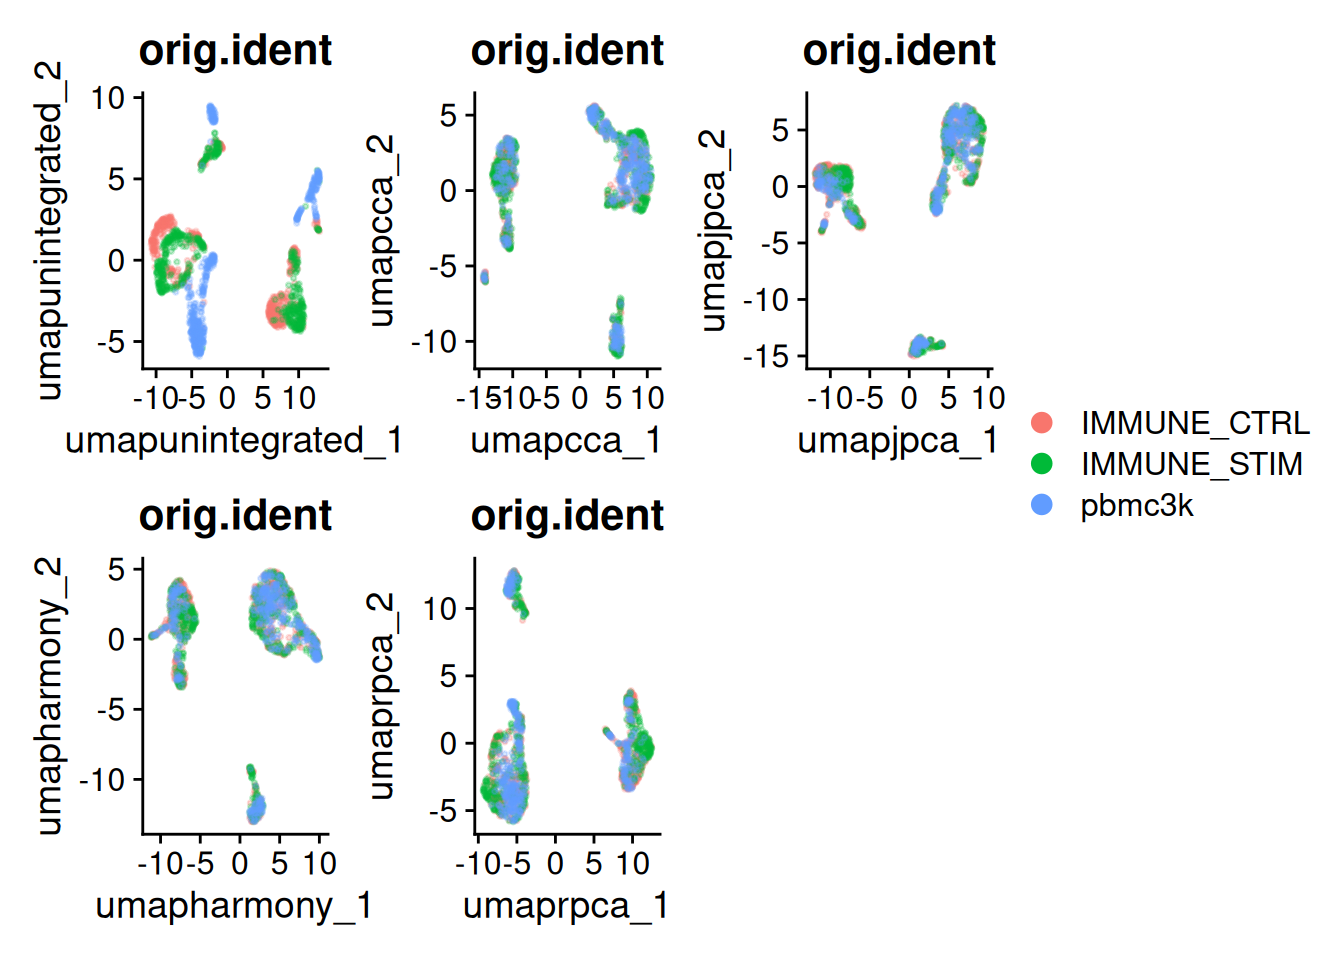
\includegraphics[keepaspectratio]{Intro_files/figure-pdf/unnamed-chunk-36-1.pdf}}

Once integrative analysis is complete, you can rejoin the layers - which
collapses the individual datasets together and recreates the original
counts and data layers. You will need to do this before performing any
differential expression analysis. However, you can always re-split the
layers in case you would like to re-perform integrative analysis.

\begin{Shaded}
\begin{Highlighting}[]
\NormalTok{all\_data\_sub }\OtherTok{\textless{}{-}} \FunctionTok{JoinLayers}\NormalTok{(all\_data\_sub, }\AttributeTok{assay =}\StringTok{\textquotesingle{}RNA\textquotesingle{}}\NormalTok{)}
\end{Highlighting}
\end{Shaded}

We can also see how well the pre-populated cell annotations and Seurat
clusters agree, with a table where the rpca\_clusters are rows and cell
annotations are rows:

\begin{Shaded}
\begin{Highlighting}[]
\FunctionTok{table}\NormalTok{(all\_data\_sub}\SpecialCharTok{$}\NormalTok{seurat\_annotations, all\_data\_sub}\SpecialCharTok{$}\NormalTok{rpca\_clusters)}
\end{Highlighting}
\end{Shaded}

\begin{verbatim}
              
                 0   1   2   3   4   5   6   7
  B              0   0 125   0   0   0   0   0
  B Activated    0   0  28   0   0   0   0   0
  CD14 Mono    294   1   0   0   0   9   0   0
  CD14+ Mono    82   0   0   0   0   3   0   0
  CD16 Mono      2   0   0   0   0  78   0   0
  CD4 Memory T   0 119   0   0   5   0  10   0
  CD4 Naive T    0  37   1   0 121   0  24   0
  CD8 T          0  16   1  74   1   0   2   0
  DC             7   0   1   0   0   0   0  31
  Eryth          1   2   0   0   0   2   0   0
  FCGR3A+ Mono   1   0   0   0   0  21   0   0
  Memory CD4 T   0  66   1   1   1   0  11   0
  Mk             5   5   0   0   3   3   1   0
  Naive CD4 T    0 114   0   1  12   0   4   0
  NK             0   0   0  70   0   0   2   0
  pDC            0   1   6   0   1   0   1   0
  Platelet       1   0   0   0   0   0   0   0
  T activated    0   2   1   1   0   0  43   0
\end{verbatim}

We can also compare dimplots with different labels:

\begin{Shaded}
\begin{Highlighting}[]
\FunctionTok{Idents}\NormalTok{(all\_data\_sub) }\OtherTok{\textless{}{-}} \StringTok{\textquotesingle{}seurat\_annotations\textquotesingle{}}
\NormalTok{plot1 }\OtherTok{\textless{}{-}} \FunctionTok{DimPlot}\NormalTok{(all\_data\_sub) }
\FunctionTok{LabelClusters}\NormalTok{(plot1, }\AttributeTok{id =} \StringTok{"ident"}\NormalTok{, }\AttributeTok{box=} \ConstantTok{TRUE}\NormalTok{, }\AttributeTok{size =} \DecValTok{5}\NormalTok{, }\AttributeTok{repel =}\NormalTok{ T, }\AttributeTok{fill =} \StringTok{\textquotesingle{}white\textquotesingle{}}\NormalTok{)}
\end{Highlighting}
\end{Shaded}

\pandocbounded{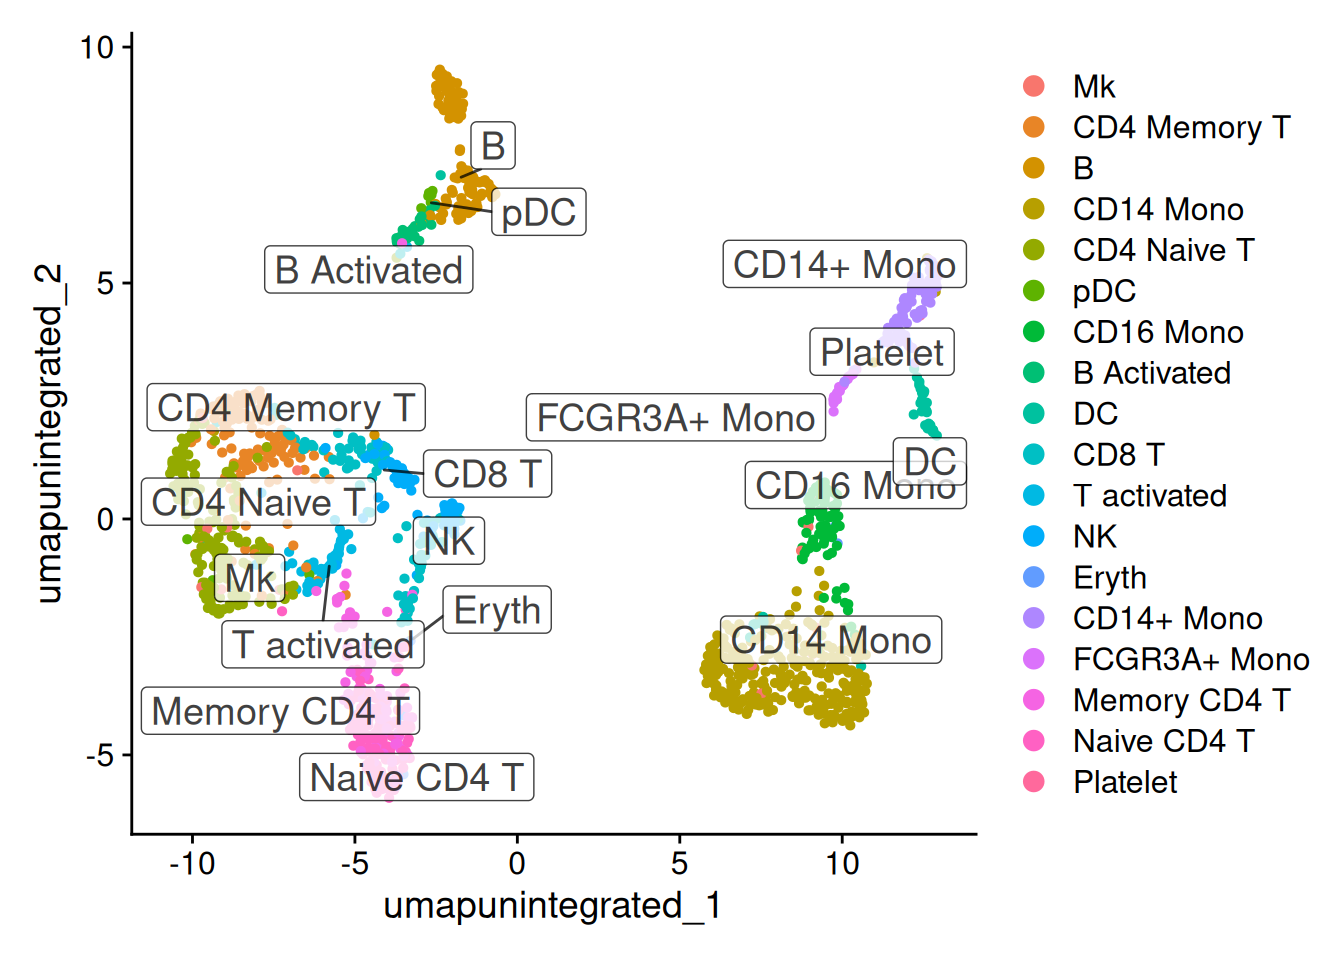
\includegraphics[keepaspectratio]{Intro_files/figure-pdf/unnamed-chunk-39-1.pdf}}

\begin{Shaded}
\begin{Highlighting}[]
\FunctionTok{Idents}\NormalTok{(all\_data\_sub) }\OtherTok{\textless{}{-}} \StringTok{\textquotesingle{}rpca\_clusters\textquotesingle{}}
\NormalTok{plot2 }\OtherTok{\textless{}{-}} \FunctionTok{DimPlot}\NormalTok{(all\_data\_sub) }
\FunctionTok{LabelClusters}\NormalTok{(plot2, }\AttributeTok{id =} \StringTok{"ident"}\NormalTok{, }\AttributeTok{box=} \ConstantTok{TRUE}\NormalTok{, }\AttributeTok{size =} \DecValTok{5}\NormalTok{, }\AttributeTok{repel =}\NormalTok{ T, }\AttributeTok{fill =} \StringTok{\textquotesingle{}white\textquotesingle{}}\NormalTok{)}
\end{Highlighting}
\end{Shaded}

\pandocbounded{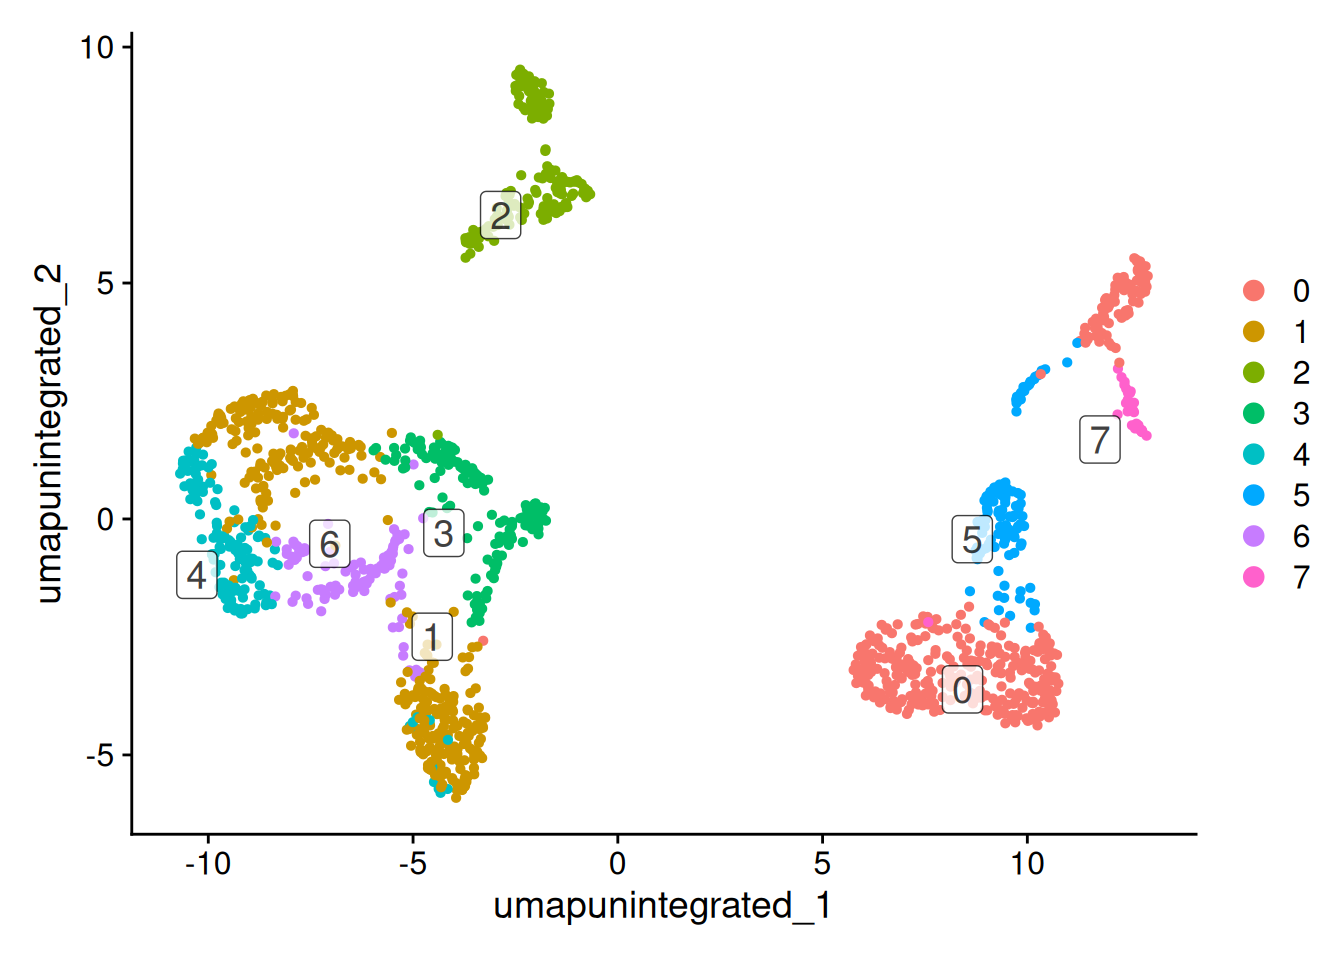
\includegraphics[keepaspectratio]{Intro_files/figure-pdf/unnamed-chunk-39-2.pdf}}

\subsection{Clustering resolution
selection}\label{clustering-resolution-selection}

You can use the \texttt{clustree} package to get a sense of how the
resolution to select will impact the clustering.

First, try running the clustering across a range of resolutions:

\begin{Shaded}
\begin{Highlighting}[]
\NormalTok{resolution.range }\OtherTok{\textless{}{-}} \FunctionTok{seq}\NormalTok{(}\AttributeTok{from =} \DecValTok{0}\NormalTok{, }\AttributeTok{to =} \FloatTok{1.2}\NormalTok{, }\AttributeTok{by =} \FloatTok{0.1}\NormalTok{)}
\NormalTok{tree }\OtherTok{\textless{}{-}} \FunctionTok{FindClusters}\NormalTok{(all\_data\_sub, }\AttributeTok{resolution =}\NormalTok{ resolution.range)}
\end{Highlighting}
\end{Shaded}

Then we can look at the clustering tree.

\begin{Shaded}
\begin{Highlighting}[]
\FunctionTok{clustree}\NormalTok{(tree)}
\end{Highlighting}
\end{Shaded}

\pandocbounded{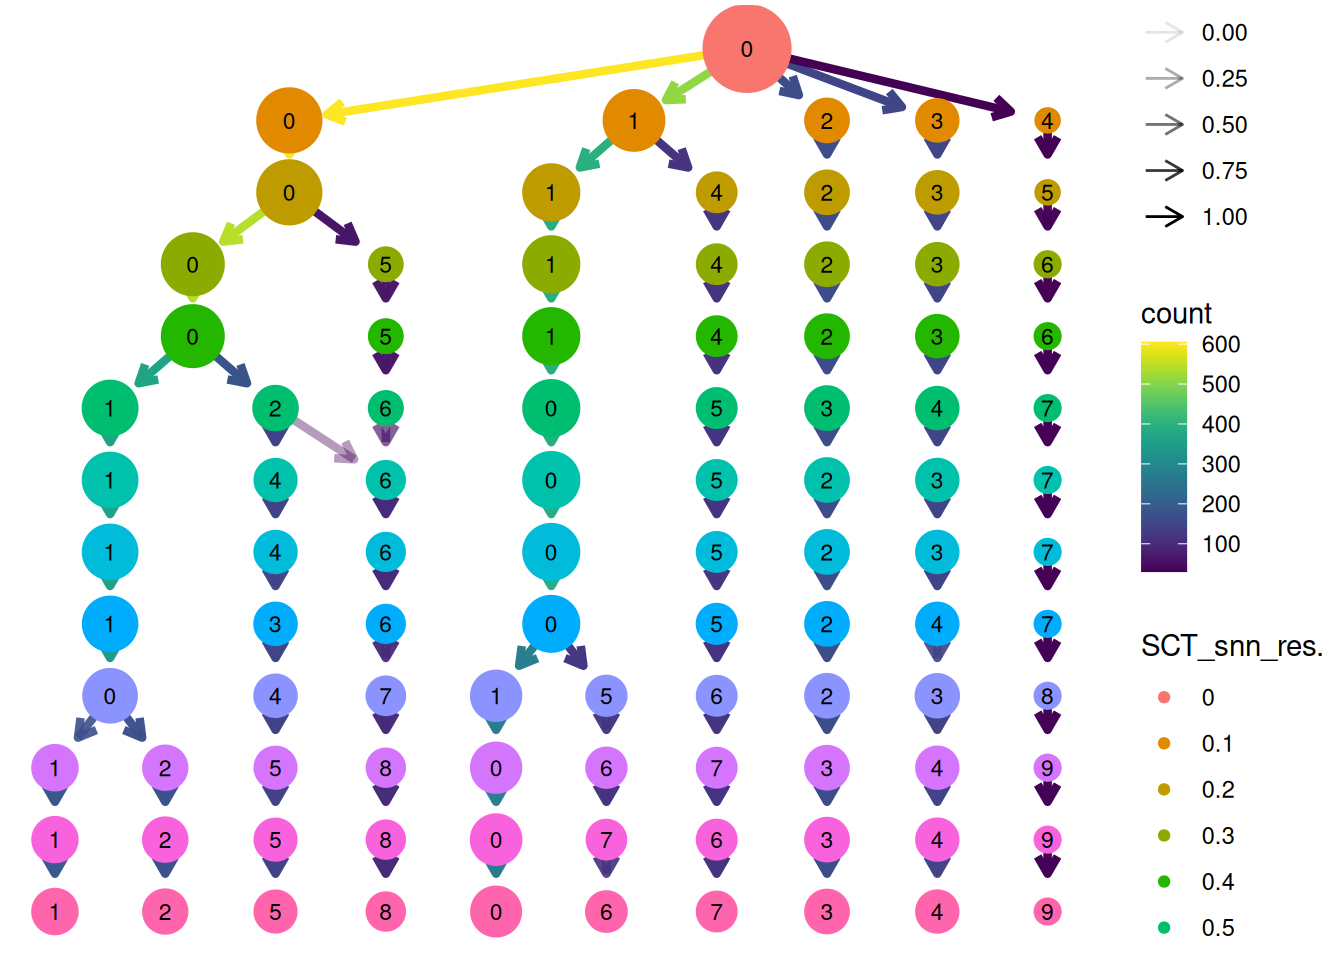
\includegraphics[keepaspectratio]{Intro_files/figure-pdf/unnamed-chunk-41-1.pdf}}

The size of the dots indicates how many cells are in each cluster and
the color indicates the resolution used. At the top is showing us the
clustering results from \texttt{resolution\ =\ 0}, and moving down the
tree we can see clusters splitting out into smaller sub-clusters as we
reach higher resolutions. If you see situations where clusters split and
then re-cluster, this might be a sign that you are getting into
over-clustering territory.

\section{Differential Expression
Analysis}\label{differential-expression-analysis}

The bulk of Seurat's differential expression features can be accessed
through the \texttt{FindMarkers()} or \texttt{FindAllMarkers()}
functions. By default, Seurat performs differential expression (DE)
testing based on the non-parametric Wilcoxon rank sum test. To test for
DE genes between two specific groups of cells, use
\texttt{FindMarkers()} and specify the \texttt{ident.1} and
\texttt{ident.2} parameters. Use \texttt{FindAllMarkers()} to test each
\texttt{ident} to all other idents. If you have a more complex
experimental design, Seurat might not be the best choice and you can
come visit us at office hours to discuss your options.

Since we normalized using SCTransform, we have to run
\texttt{PrepSCTFindMarkers()} first. Given a merged object with multiple
SCT models, this function uses minimum of the median UMI (calculated
using the raw UMI counts) of individual objects to reverse the
individual SCT regression model using minimum of median UMI as the
sequencing depth covariate. The counts slot of the SCT assay is replaced
with recorrected counts and the data slot is replaced with log1p of
recorrected counts. Then set the \texttt{DefaultAssay} to be the RNA
assay.

\begin{Shaded}
\begin{Highlighting}[]
\FunctionTok{Idents}\NormalTok{(all\_data\_sub) }\OtherTok{\textless{}{-}} \StringTok{"orig.ident"}
\NormalTok{all\_data\_sub }\OtherTok{\textless{}{-}} \FunctionTok{PrepSCTFindMarkers}\NormalTok{(all\_data\_sub)}
\end{Highlighting}
\end{Shaded}

\begin{verbatim}
Found 3 SCT models. Recorrecting SCT counts using minimum median counts: 1636.5
\end{verbatim}

\begin{Shaded}
\begin{Highlighting}[]
\FunctionTok{DefaultAssay}\NormalTok{(all\_data\_sub) }\OtherTok{\textless{}{-}} \StringTok{"RNA"}

\NormalTok{stim\_vs\_ctrl }\OtherTok{\textless{}{-}} \FunctionTok{FindMarkers}\NormalTok{(all\_data\_sub, }\AttributeTok{ident.1 =} \StringTok{"IMMUNE\_STIM"}\NormalTok{, }\AttributeTok{ident.2 =} \StringTok{"IMMUNE\_CTRL"}\NormalTok{)}
\FunctionTok{head}\NormalTok{(stim\_vs\_ctrl }\SpecialCharTok{\%\textgreater{}\%}\NormalTok{ dplyr}\SpecialCharTok{::}\FunctionTok{filter}\NormalTok{(p\_val\_adj }\SpecialCharTok{\textless{}}\NormalTok{ .}\DecValTok{05} \SpecialCharTok{\&}\NormalTok{ avg\_log2FC }\SpecialCharTok{\textgreater{}} \DecValTok{1}\NormalTok{))}
\end{Highlighting}
\end{Shaded}

\begin{verbatim}
              p_val avg_log2FC pct.1 pct.2     p_val_adj
IFIT3 2.304328e-158   56.44791 0.934 0.060 3.445661e-154
ISG15 7.479361e-152  399.60034 0.988 0.322 1.118389e-147
IFIT1 9.416450e-152   53.38548 0.904 0.036 1.408042e-147
ISG20 2.594336e-148   27.87676 0.988 0.410 3.879311e-144
IFI6  1.526537e-141   28.76951 0.942 0.180 2.282630e-137
MX1   8.625130e-138   15.71071 0.894 0.098 1.289716e-133
\end{verbatim}

The results data frame has the following columns :

\begin{verbatim}
p_val : p-value (unadjusted)
avg_log2FC : log fold-change of the average expression between the two groups. Positive values indicate that the feature is more highly expressed in the first group.
pct.1 : The percentage of cells where the feature is detected in the first group
pct.2 : The percentage of cells where the feature is detected in the second group
p_val_adj : Adjusted p-value, based on Bonferroni correction using all features in the dataset.
\end{verbatim}

If the \texttt{ident.2} argument is omitted, \texttt{FindMarkers} will
test for differentially expressed features between the group specified
by \texttt{ident.1} and all other cells. Additionally, the parameter
\texttt{only.pos} can be set to TRUE to only search for positive
markers, i.e.~features that are more highly expressed in the ident.1
group.

\begin{Shaded}
\begin{Highlighting}[]
\NormalTok{stim\_vs\_all }\OtherTok{\textless{}{-}} \FunctionTok{FindMarkers}\NormalTok{(all\_data\_sub, }\AttributeTok{ident.1 =} \StringTok{"IMMUNE\_STIM"}\NormalTok{, }\AttributeTok{only.pos =}\NormalTok{ T)}
\FunctionTok{head}\NormalTok{(stim\_vs\_all }\SpecialCharTok{\%\textgreater{}\%}\NormalTok{ dplyr}\SpecialCharTok{::}\FunctionTok{filter}\NormalTok{(p\_val\_adj }\SpecialCharTok{\textless{}}\NormalTok{ .}\DecValTok{05} \SpecialCharTok{\&}\NormalTok{ avg\_log2FC }\SpecialCharTok{\textgreater{}} \DecValTok{1}\NormalTok{))}
\end{Highlighting}
\end{Shaded}

\begin{verbatim}
              p_val avg_log2FC pct.1 pct.2     p_val_adj
IFIT3 6.980485e-236   56.59723 0.934 0.084 1.043792e-231
IFIT1 7.150314e-227   54.24998 0.904 0.064 1.069187e-222
ISG20 8.852470e-204   20.15248 0.988 0.428 1.323710e-199
ISG15 8.337627e-203  400.53542 0.988 0.384 1.246725e-198
IFIT2 9.924276e-182   41.32732 0.756 0.043 1.483977e-177
RSAD2 6.594093e-161   56.68649 0.710 0.053 9.860147e-157
\end{verbatim}

We can switch idents to find marker genes for the clusters:

\begin{Shaded}
\begin{Highlighting}[]
\FunctionTok{Idents}\NormalTok{(all\_data\_sub) }\OtherTok{\textless{}{-}} \StringTok{\textquotesingle{}rpca\_clusters\textquotesingle{}}
\end{Highlighting}
\end{Shaded}

Use \texttt{FindAllMarkers} to compare each cluster to all the other
clusters. For the sake of speed, we are selecting only positive genes
that are expressed in at least 90\% of the cells for a given cluster:

\begin{Shaded}
\begin{Highlighting}[]
\NormalTok{rpca\_markers }\OtherTok{\textless{}{-}} \FunctionTok{FindAllMarkers}\NormalTok{(all\_data\_sub, }\AttributeTok{min.pct =}\NormalTok{ .}\DecValTok{90}\NormalTok{, }\AttributeTok{only.pos=}\ConstantTok{TRUE}\NormalTok{)}
\end{Highlighting}
\end{Shaded}

\begin{verbatim}
Calculating cluster 0
\end{verbatim}

\begin{verbatim}
Calculating cluster 1
\end{verbatim}

\begin{verbatim}
Calculating cluster 2
\end{verbatim}

\begin{verbatim}
Calculating cluster 3
\end{verbatim}

\begin{verbatim}
Calculating cluster 4
\end{verbatim}

\begin{verbatim}
Calculating cluster 5
\end{verbatim}

\begin{verbatim}
Calculating cluster 6
\end{verbatim}

\begin{verbatim}
Calculating cluster 7
\end{verbatim}

Look at the marker genes with the biggest fold change per cluster

\begin{Shaded}
\begin{Highlighting}[]
\NormalTok{top\_cluster\_markers }\OtherTok{\textless{}{-}} 
\NormalTok{  rpca\_markers }\SpecialCharTok{\%\textgreater{}\%} 
  \FunctionTok{group\_by}\NormalTok{(cluster) }\SpecialCharTok{\%\textgreater{}\%}
\NormalTok{  dplyr}\SpecialCharTok{::}\FunctionTok{filter}\NormalTok{(p\_val\_adj }\SpecialCharTok{\textless{}=} \FloatTok{0.05}\NormalTok{) }\SpecialCharTok{\%\textgreater{}\%}
\NormalTok{  dplyr}\SpecialCharTok{::}\FunctionTok{filter}\NormalTok{(avg\_log2FC }\SpecialCharTok{\textgreater{}} \DecValTok{1}\NormalTok{) }\SpecialCharTok{\%\textgreater{}\%} 
\NormalTok{  dplyr}\SpecialCharTok{::}\FunctionTok{filter}\NormalTok{(pct}\FloatTok{.1} \SpecialCharTok{\textgreater{}}\NormalTok{ .}\DecValTok{9}\NormalTok{) }\SpecialCharTok{\%\textgreater{}\%}
  \FunctionTok{slice\_max}\NormalTok{(}\AttributeTok{n =} \DecValTok{2}\NormalTok{, }\AttributeTok{order\_by =} \FunctionTok{abs}\NormalTok{(avg\_log2FC))}
\NormalTok{top\_cluster\_markers}
\end{Highlighting}
\end{Shaded}

\begin{verbatim}
# A tibble: 13 x 7
# Groups:   cluster [7]
       p_val avg_log2FC pct.1 pct.2 p_val_adj cluster gene   
       <dbl>      <dbl> <dbl> <dbl>     <dbl> <fct>   <chr>  
 1 2.03e-162     335.   1     0.921 3.03e-158 0       FTL    
 2 3.85e-140     108.   0.954 0.322 5.76e-136 0       NPC2   
 3 4.47e- 40      51.7  0.983 0.859 6.69e- 36 1       RPS5   
 4 1.09e- 76      44.9  1     0.97  1.62e- 72 1       RPL3   
 5 2.83e-  6      57.8  0.988 0.982 4.23e-  2 2       TPT1   
 6 6.89e- 17      27.9  0.994 0.926 1.03e- 12 2       PTMA   
 7 3.95e-172      62.4  0.946 0.086 5.90e-168 3       NKG7   
 8 4.74e- 17      52.9  1     0.985 7.08e- 13 3       HLA-A  
 9 7.01e- 47       1.09 0.917 0.421 1.05e- 42 4       GIMAP7 
10 5.59e- 15     149.   1     1     8.36e- 11 5       MALAT1 
11 3.89e- 10      49.7  1     0.991 5.82e-  6 5       RPS19  
12 1.13e- 22     234.   1     0.566 1.69e- 18 7       HLA-DRA
13 2.89e- 21     225.   1     0.745 4.32e- 17 7       CD74   
\end{verbatim}

Make a \texttt{FeaturePlot} to look at the expression of specific genes.
It will plot the \texttt{data} slot from the default assay. We can
switch the default assay to SCT first and specify that we want to use
the \texttt{data} slot (log1p(counts)):

\begin{Shaded}
\begin{Highlighting}[]
\FunctionTok{DefaultAssay}\NormalTok{(all\_data\_sub) }\OtherTok{\textless{}{-}} \StringTok{"SCT"}

\FunctionTok{FeaturePlot}\NormalTok{(all\_data\_sub, }\AttributeTok{features =} \FunctionTok{c}\NormalTok{(}\StringTok{"CCL3"}\NormalTok{), }\AttributeTok{reduction =} \StringTok{\textquotesingle{}umap.rpca\textquotesingle{}}\NormalTok{, }\AttributeTok{order =}\NormalTok{ T, }\AttributeTok{slot =} \StringTok{\textquotesingle{}data\textquotesingle{}}\NormalTok{)}
\end{Highlighting}
\end{Shaded}

\pandocbounded{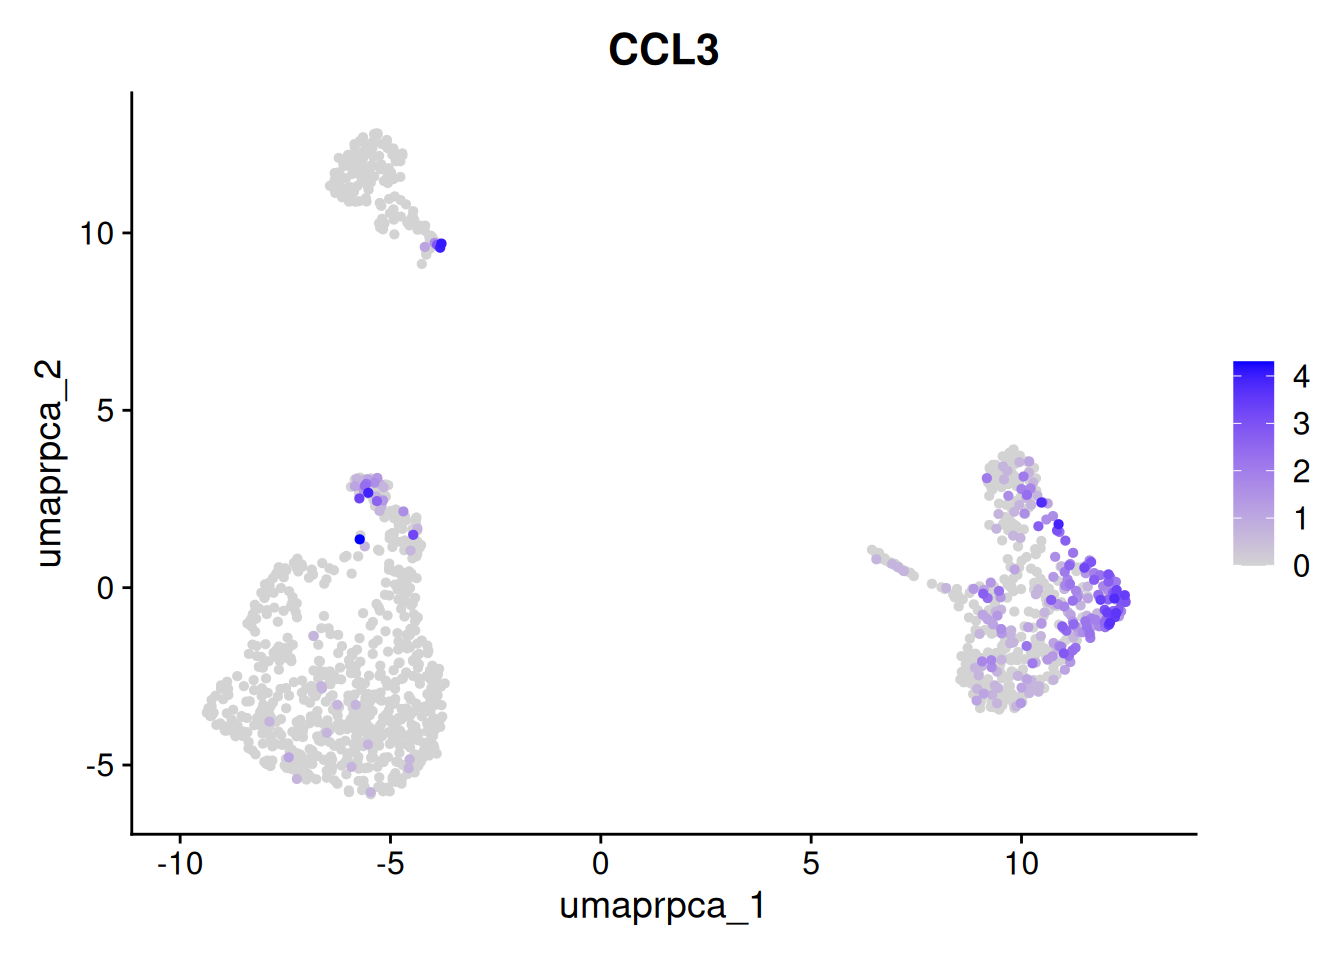
\includegraphics[keepaspectratio]{Intro_files/figure-pdf/unnamed-chunk-47-1.pdf}}

We can adjust the default colors and use one of the \texttt{viridis}
palettes:

\begin{Shaded}
\begin{Highlighting}[]
\FunctionTok{FeaturePlot}\NormalTok{(all\_data\_sub, }\AttributeTok{features =} \FunctionTok{c}\NormalTok{(}\StringTok{"CCL3"}\NormalTok{), }\AttributeTok{reduction =} \StringTok{\textquotesingle{}umap.rpca\textquotesingle{}}\NormalTok{, }\AttributeTok{order =}\NormalTok{ T, }\AttributeTok{slot =} \StringTok{\textquotesingle{}data\textquotesingle{}}\NormalTok{) }\SpecialCharTok{\&}\NormalTok{ ggplot2}\SpecialCharTok{::}\FunctionTok{scale\_color\_gradientn}\NormalTok{(}\AttributeTok{colors =}\NormalTok{ viridis}\SpecialCharTok{::}\FunctionTok{turbo}\NormalTok{(}\AttributeTok{n =} \DecValTok{10}\NormalTok{, }\AttributeTok{direction =} \DecValTok{1}\NormalTok{))}
\end{Highlighting}
\end{Shaded}

\begin{verbatim}
Scale for colour is already present.
Adding another scale for colour, which will replace the existing scale.
\end{verbatim}

\pandocbounded{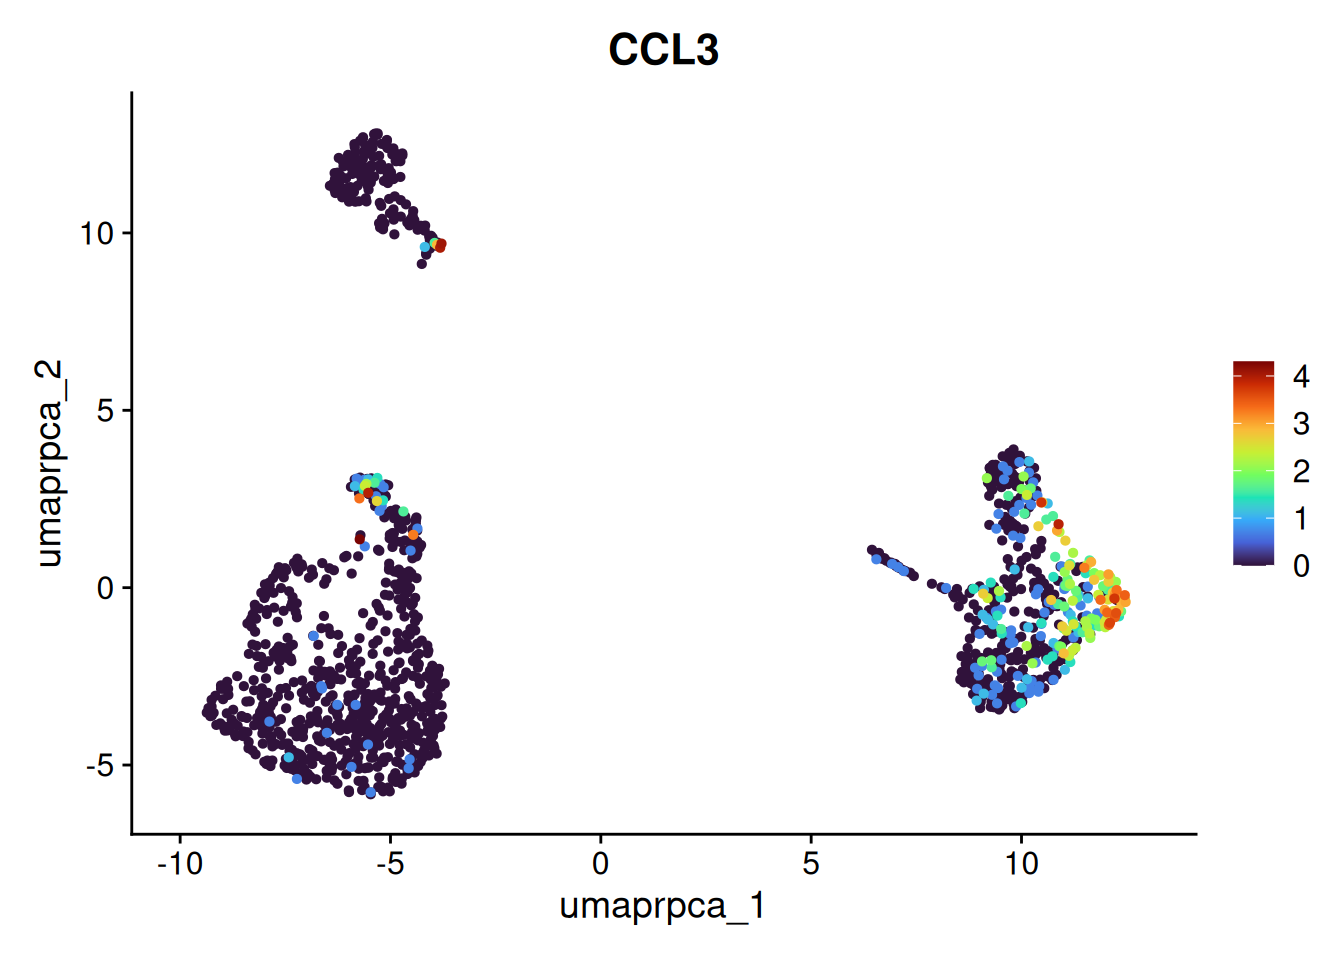
\includegraphics[keepaspectratio]{Intro_files/figure-pdf/unnamed-chunk-48-1.pdf}}

We can add the cluster labels:

\begin{Shaded}
\begin{Highlighting}[]
\FunctionTok{FeaturePlot}\NormalTok{(all\_data\_sub, }\AttributeTok{features =} \FunctionTok{c}\NormalTok{(}\StringTok{"CCL3"}\NormalTok{), }\AttributeTok{reduction =} \StringTok{\textquotesingle{}umap.rpca\textquotesingle{}}\NormalTok{, }\AttributeTok{order =}\NormalTok{ T, }\AttributeTok{slot =} \StringTok{\textquotesingle{}data\textquotesingle{}}\NormalTok{, }\AttributeTok{label =} \ConstantTok{TRUE}\NormalTok{, }\AttributeTok{repel =} \ConstantTok{TRUE}\NormalTok{) }\SpecialCharTok{\&}\NormalTok{ ggplot2}\SpecialCharTok{::}\FunctionTok{scale\_color\_gradientn}\NormalTok{(}\AttributeTok{colors =}\NormalTok{ viridis}\SpecialCharTok{::}\FunctionTok{turbo}\NormalTok{(}\AttributeTok{n =} \DecValTok{10}\NormalTok{, }\AttributeTok{direction =} \DecValTok{1}\NormalTok{))}
\end{Highlighting}
\end{Shaded}

\begin{verbatim}
Scale for colour is already present.
Adding another scale for colour, which will replace the existing scale.
\end{verbatim}

\pandocbounded{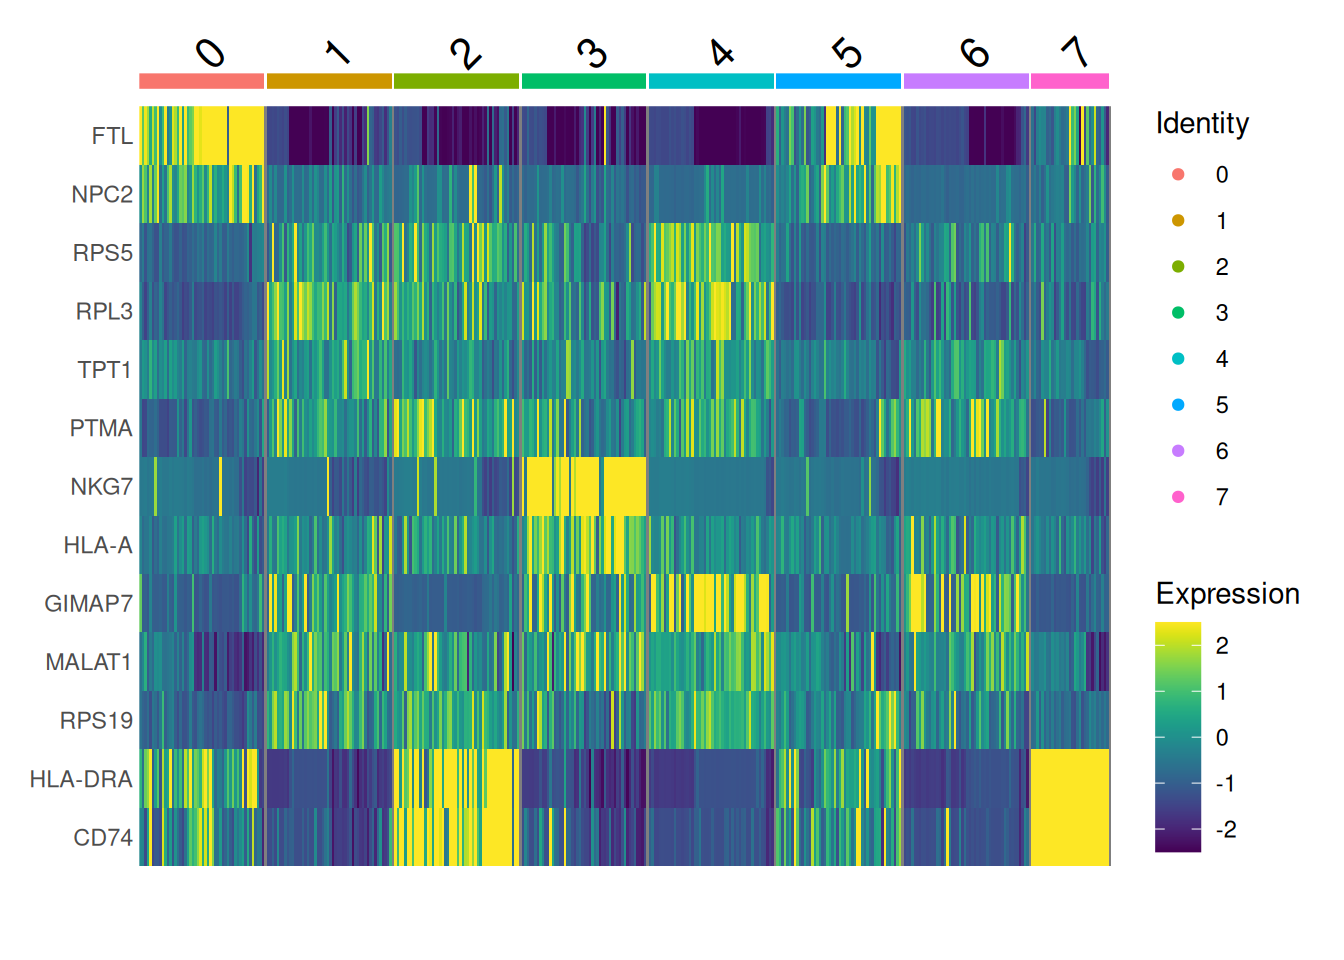
\includegraphics[keepaspectratio]{Intro_files/figure-pdf/unnamed-chunk-49-1.pdf}}

The labels are a bit hard to see. We can use \texttt{RColorBrewer}
palettes instead and specify that we want to drop the colors on the
extreme ends of the \texttt{Spectral} palette:

\begin{Shaded}
\begin{Highlighting}[]
\FunctionTok{FeaturePlot}\NormalTok{(all\_data\_sub, }\AttributeTok{features =} \FunctionTok{c}\NormalTok{(}\StringTok{"CCL3"}\NormalTok{), }\AttributeTok{reduction =} \StringTok{\textquotesingle{}umap.rpca\textquotesingle{}}\NormalTok{, }\AttributeTok{order =}\NormalTok{ T, }\AttributeTok{slot =} \StringTok{\textquotesingle{}data\textquotesingle{}}\NormalTok{, }\AttributeTok{label =} \ConstantTok{TRUE}\NormalTok{, }\AttributeTok{repel =} \ConstantTok{TRUE}\NormalTok{) }\SpecialCharTok{\&}\NormalTok{ ggplot2}\SpecialCharTok{::}\FunctionTok{scale\_color\_gradientn}\NormalTok{(}\AttributeTok{colors =} \FunctionTok{rev}\NormalTok{(}\FunctionTok{brewer.pal}\NormalTok{(}\DecValTok{10}\NormalTok{, }\StringTok{\textquotesingle{}Spectral\textquotesingle{}}\NormalTok{))[}\DecValTok{3}\SpecialCharTok{:}\DecValTok{8}\NormalTok{])}
\end{Highlighting}
\end{Shaded}

\begin{verbatim}
Scale for colour is already present.
Adding another scale for colour, which will replace the existing scale.
\end{verbatim}

\pandocbounded{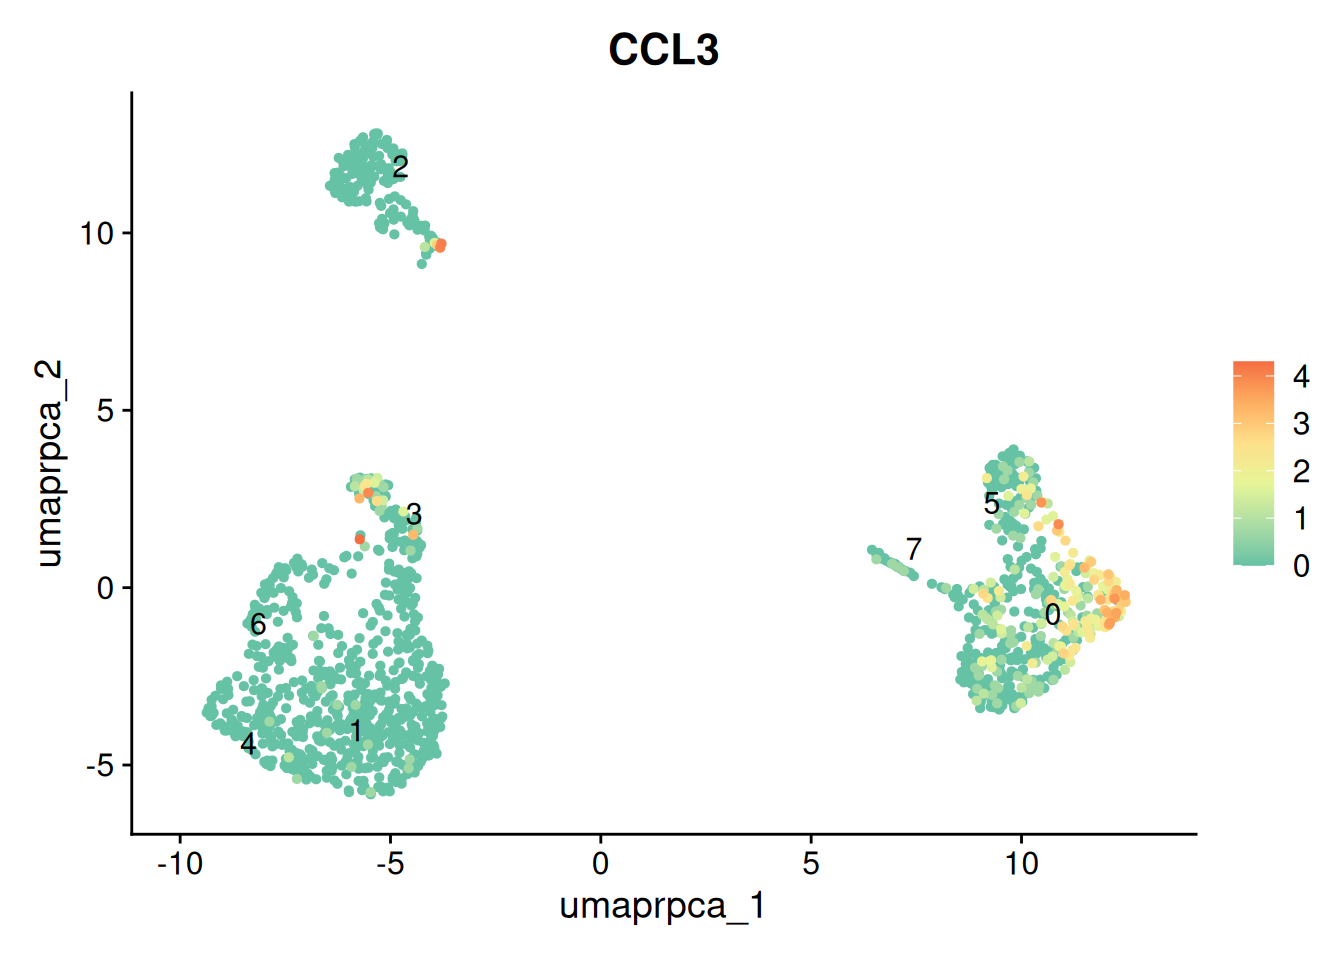
\includegraphics[keepaspectratio]{Intro_files/figure-pdf/unnamed-chunk-50-1.pdf}}

And add a legend title

\begin{Shaded}
\begin{Highlighting}[]
\FunctionTok{FeaturePlot}\NormalTok{(all\_data\_sub, }\AttributeTok{features =} \FunctionTok{c}\NormalTok{(}\StringTok{"CCL3"}\NormalTok{), }\AttributeTok{reduction =} \StringTok{\textquotesingle{}umap.rpca\textquotesingle{}}\NormalTok{, }\AttributeTok{order =}\NormalTok{ T, }\AttributeTok{slot =} \StringTok{\textquotesingle{}data\textquotesingle{}}\NormalTok{, }\AttributeTok{label =} \ConstantTok{TRUE}\NormalTok{, }\AttributeTok{repel =} \ConstantTok{TRUE}\NormalTok{) }\SpecialCharTok{\&}\NormalTok{ ggplot2}\SpecialCharTok{::}\FunctionTok{scale\_color\_gradientn}\NormalTok{(}\AttributeTok{colors =} \FunctionTok{rev}\NormalTok{(}\FunctionTok{brewer.pal}\NormalTok{(}\DecValTok{10}\NormalTok{, }\StringTok{\textquotesingle{}Spectral\textquotesingle{}}\NormalTok{))[}\DecValTok{3}\SpecialCharTok{:}\DecValTok{8}\NormalTok{]) }\SpecialCharTok{\&}\NormalTok{ ggplot2}\SpecialCharTok{::}\FunctionTok{labs}\NormalTok{(}\AttributeTok{color =} \StringTok{"log1p}\SpecialCharTok{\textbackslash{}n}\StringTok{(counts)"}\NormalTok{)}
\end{Highlighting}
\end{Shaded}

\begin{verbatim}
Scale for colour is already present.
Adding another scale for colour, which will replace the existing scale.
\end{verbatim}

\pandocbounded{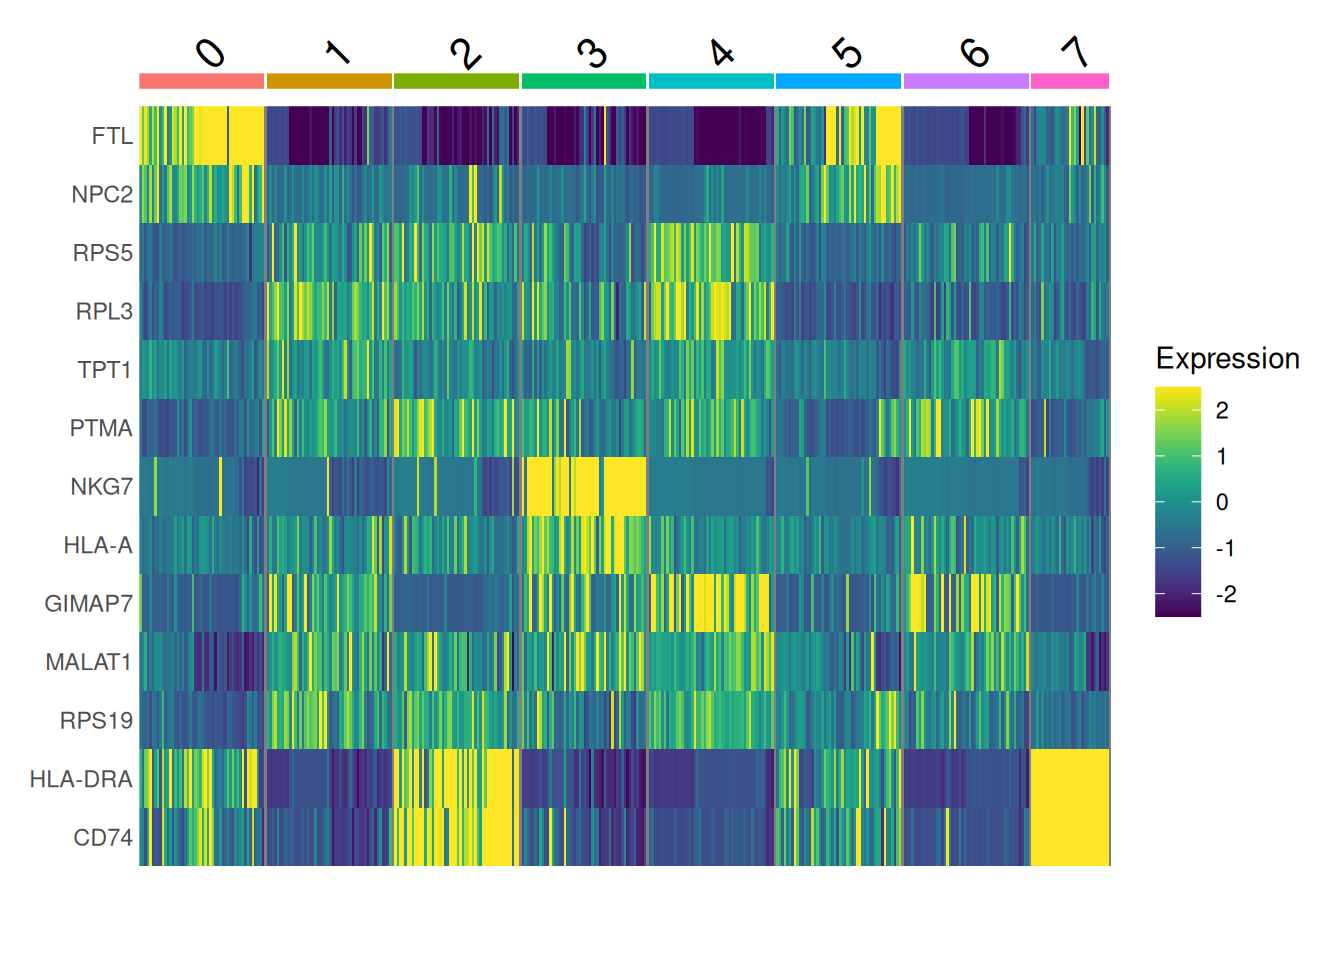
\includegraphics[keepaspectratio]{Intro_files/figure-pdf/unnamed-chunk-51-1.pdf}}

We can also make a heatmap of the cluster markers. Seurat heatmaps use
the \texttt{scale.data} slot by default.

\begin{Shaded}
\begin{Highlighting}[]
\FunctionTok{DoHeatmap}\NormalTok{(}\FunctionTok{subset}\NormalTok{(all\_data\_sub, }\AttributeTok{downsample =} \DecValTok{50}\NormalTok{), }\AttributeTok{features =}\NormalTok{ top\_cluster\_markers}\SpecialCharTok{$}\NormalTok{gene)}
\end{Highlighting}
\end{Shaded}

\pandocbounded{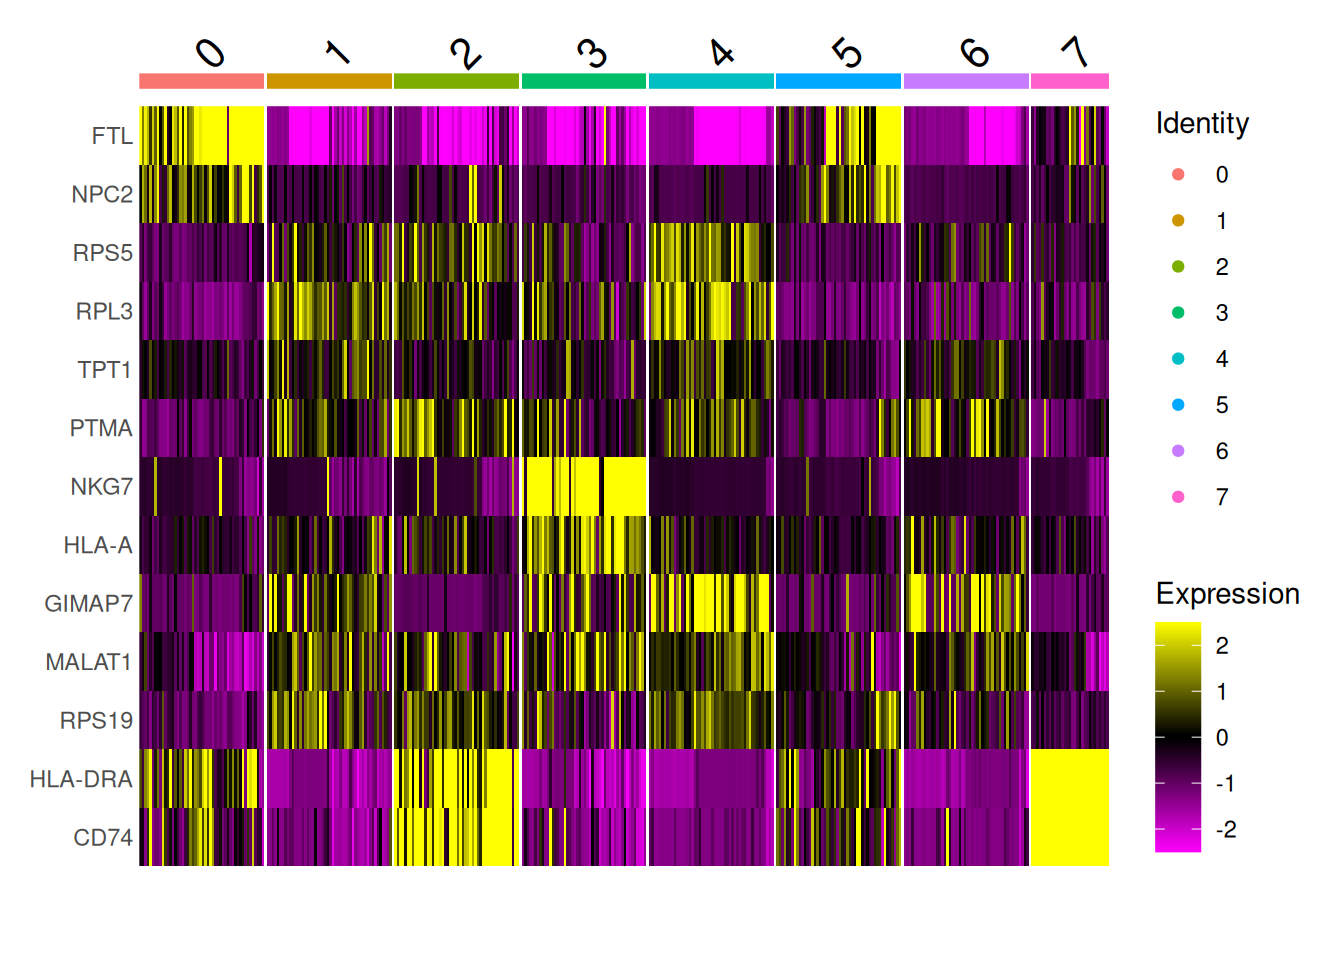
\includegraphics[keepaspectratio]{Intro_files/figure-pdf/unnamed-chunk-52-1.pdf}}

We can customize this heatmap as well:

\begin{Shaded}
\begin{Highlighting}[]
\FunctionTok{DoHeatmap}\NormalTok{(}\FunctionTok{subset}\NormalTok{(all\_data\_sub, }\AttributeTok{downsample =} \DecValTok{50}\NormalTok{), }\AttributeTok{features =}\NormalTok{ top\_cluster\_markers}\SpecialCharTok{$}\NormalTok{gene) }\SpecialCharTok{\&}\NormalTok{ viridis}\SpecialCharTok{::}\FunctionTok{scale\_fill\_viridis}\NormalTok{() }
\end{Highlighting}
\end{Shaded}

\begin{verbatim}
Scale for fill is already present.
Adding another scale for fill, which will replace the existing scale.
\end{verbatim}

\pandocbounded{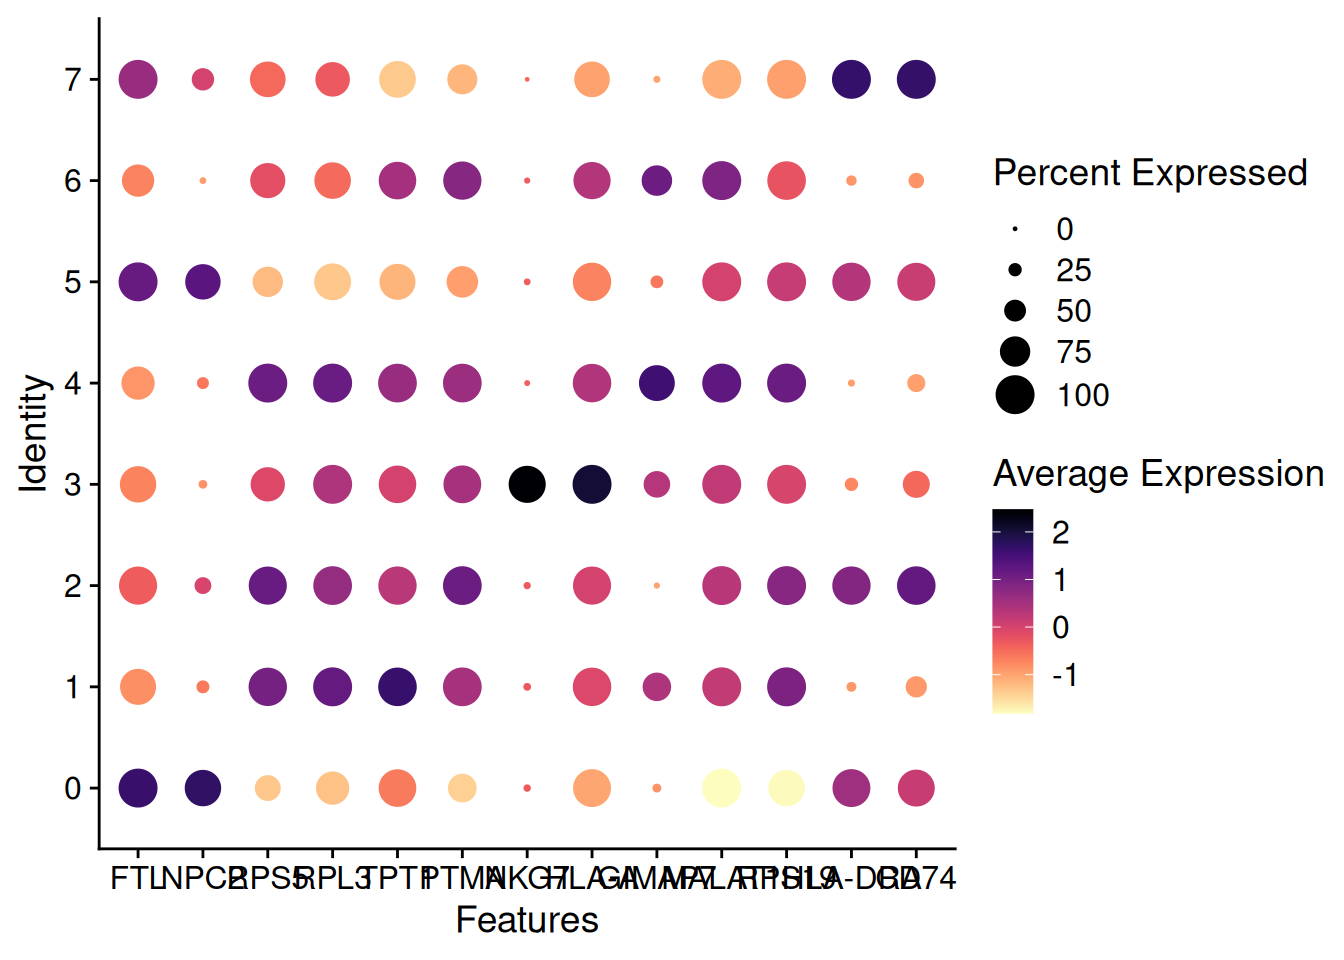
\includegraphics[keepaspectratio]{Intro_files/figure-pdf/unnamed-chunk-53-1.pdf}}

We can adjust which legends are shown, like this:

\begin{Shaded}
\begin{Highlighting}[]
\FunctionTok{DoHeatmap}\NormalTok{(}\FunctionTok{subset}\NormalTok{(all\_data\_sub, }\AttributeTok{downsample =} \DecValTok{50}\NormalTok{), }\AttributeTok{features =}\NormalTok{ top\_cluster\_markers}\SpecialCharTok{$}\NormalTok{gene) }\SpecialCharTok{\&}\NormalTok{ viridis}\SpecialCharTok{::}\FunctionTok{scale\_fill\_viridis}\NormalTok{() }\SpecialCharTok{\&}\NormalTok{ ggplot2}\SpecialCharTok{::}\FunctionTok{guides}\NormalTok{(}\AttributeTok{fill=}\ConstantTok{FALSE}\NormalTok{)}
\end{Highlighting}
\end{Shaded}

\begin{verbatim}
Scale for fill is already present.
Adding another scale for fill, which will replace the existing scale.
\end{verbatim}

\begin{verbatim}
Warning: The `<scale>` argument of `guides()` cannot be `FALSE`. Use "none" instead as
of ggplot2 3.3.4.
\end{verbatim}

\pandocbounded{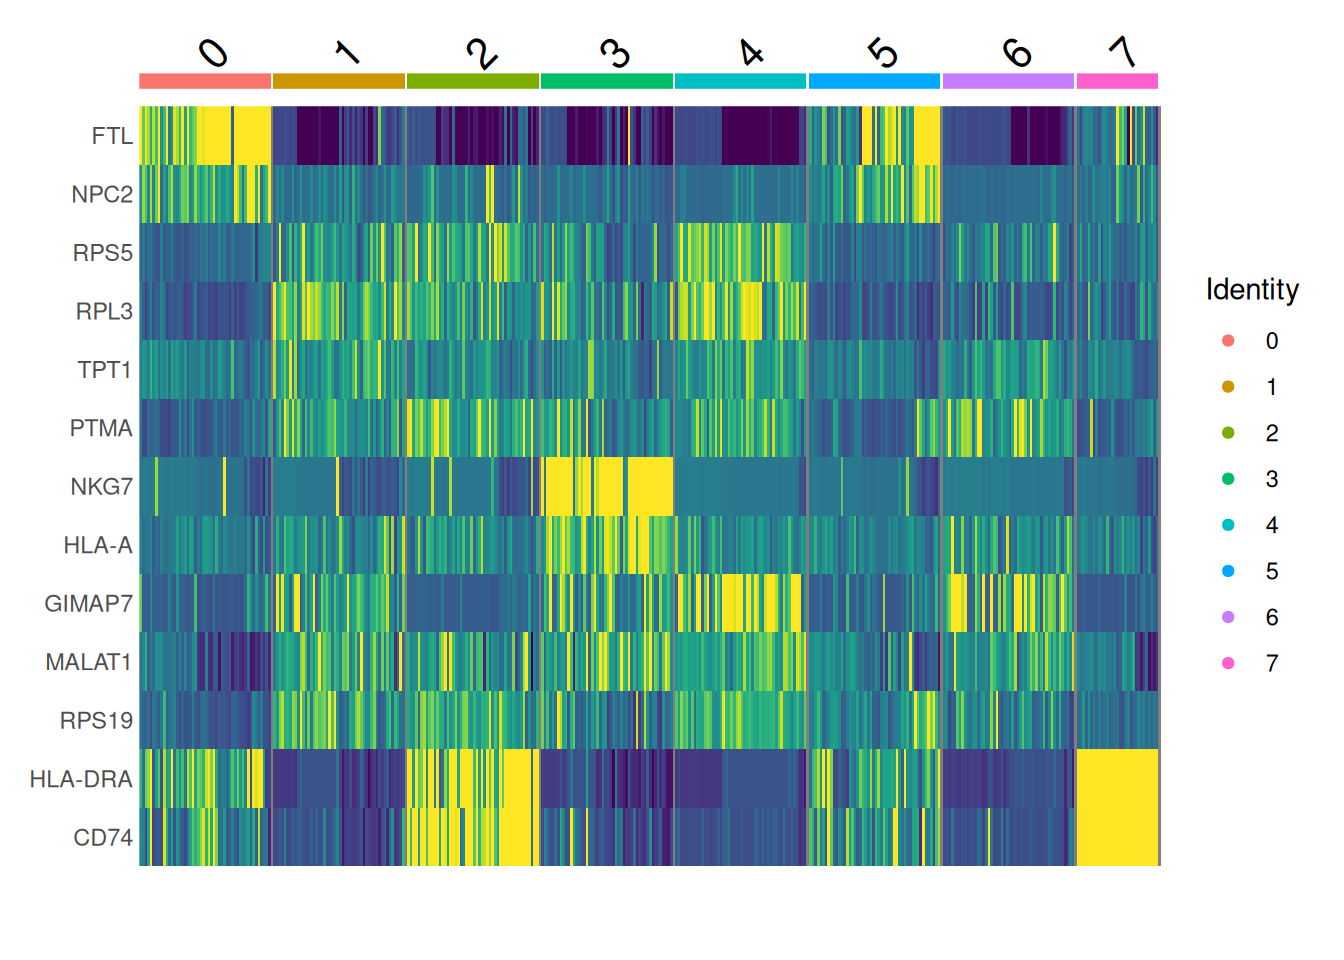
\includegraphics[keepaspectratio]{Intro_files/figure-pdf/unnamed-chunk-54-1.pdf}}

Or like this:

\begin{Shaded}
\begin{Highlighting}[]
\FunctionTok{DoHeatmap}\NormalTok{(}\FunctionTok{subset}\NormalTok{(all\_data\_sub, }\AttributeTok{downsample =} \DecValTok{50}\NormalTok{), }\AttributeTok{features =}\NormalTok{ top\_cluster\_markers}\SpecialCharTok{$}\NormalTok{gene) }\SpecialCharTok{\&}\NormalTok{ viridis}\SpecialCharTok{::}\FunctionTok{scale\_fill\_viridis}\NormalTok{() }\SpecialCharTok{\&}\NormalTok{ ggplot2}\SpecialCharTok{::}\FunctionTok{guides}\NormalTok{(}\AttributeTok{colour=}\ConstantTok{FALSE}\NormalTok{)}
\end{Highlighting}
\end{Shaded}

\begin{verbatim}
Scale for fill is already present.
Adding another scale for fill, which will replace the existing scale.
\end{verbatim}

\pandocbounded{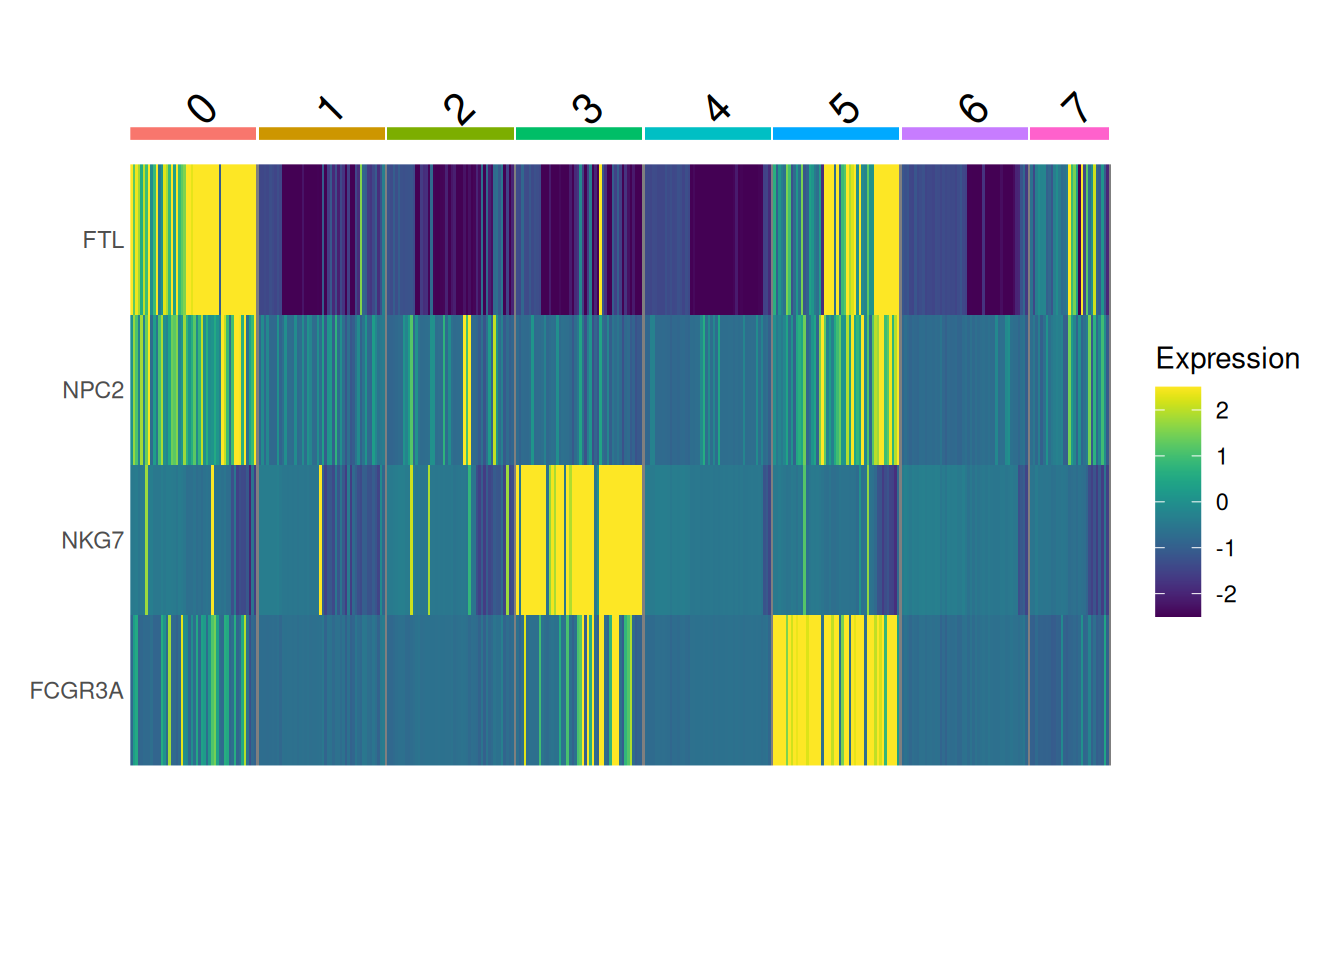
\includegraphics[keepaspectratio]{Intro_files/figure-pdf/unnamed-chunk-55-1.pdf}}

Another helpful visualization from Seurat is \texttt{DotPlot}. The size
of each dot indicates the percentage of cells expressing the feature and
the color is the average expression level. It uses the scale.data slot
by default.

\begin{Shaded}
\begin{Highlighting}[]
\FunctionTok{DotPlot}\NormalTok{(all\_data\_sub, }\AttributeTok{features =}\NormalTok{ top\_cluster\_markers}\SpecialCharTok{$}\NormalTok{gene) }
\end{Highlighting}
\end{Shaded}

\pandocbounded{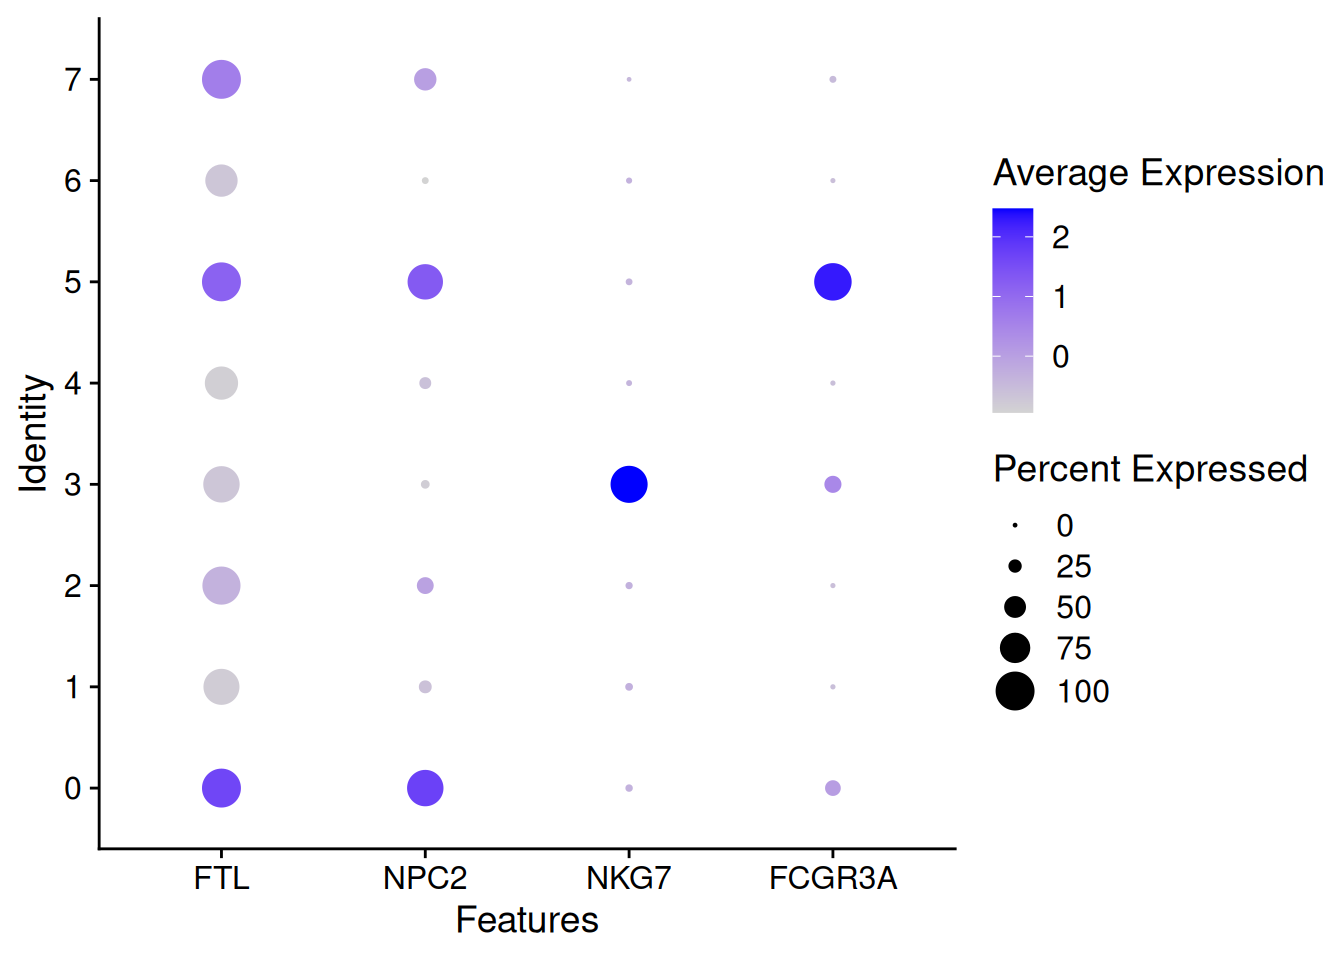
\includegraphics[keepaspectratio]{Intro_files/figure-pdf/unnamed-chunk-56-1.pdf}}

We can use more custom colors:

\begin{Shaded}
\begin{Highlighting}[]
\FunctionTok{DotPlot}\NormalTok{(all\_data\_sub, }\AttributeTok{features =}\NormalTok{ top\_cluster\_markers}\SpecialCharTok{$}\NormalTok{gene) }\SpecialCharTok{\&} 
\NormalTok{    viridis}\SpecialCharTok{::}\FunctionTok{scale\_color\_viridis}\NormalTok{(}\AttributeTok{option =} \StringTok{"magma"}\NormalTok{, }\AttributeTok{direction =} \SpecialCharTok{{-}}\DecValTok{1}\NormalTok{) }
\end{Highlighting}
\end{Shaded}

\begin{verbatim}
Scale for colour is already present.
Adding another scale for colour, which will replace the existing scale.
\end{verbatim}

\pandocbounded{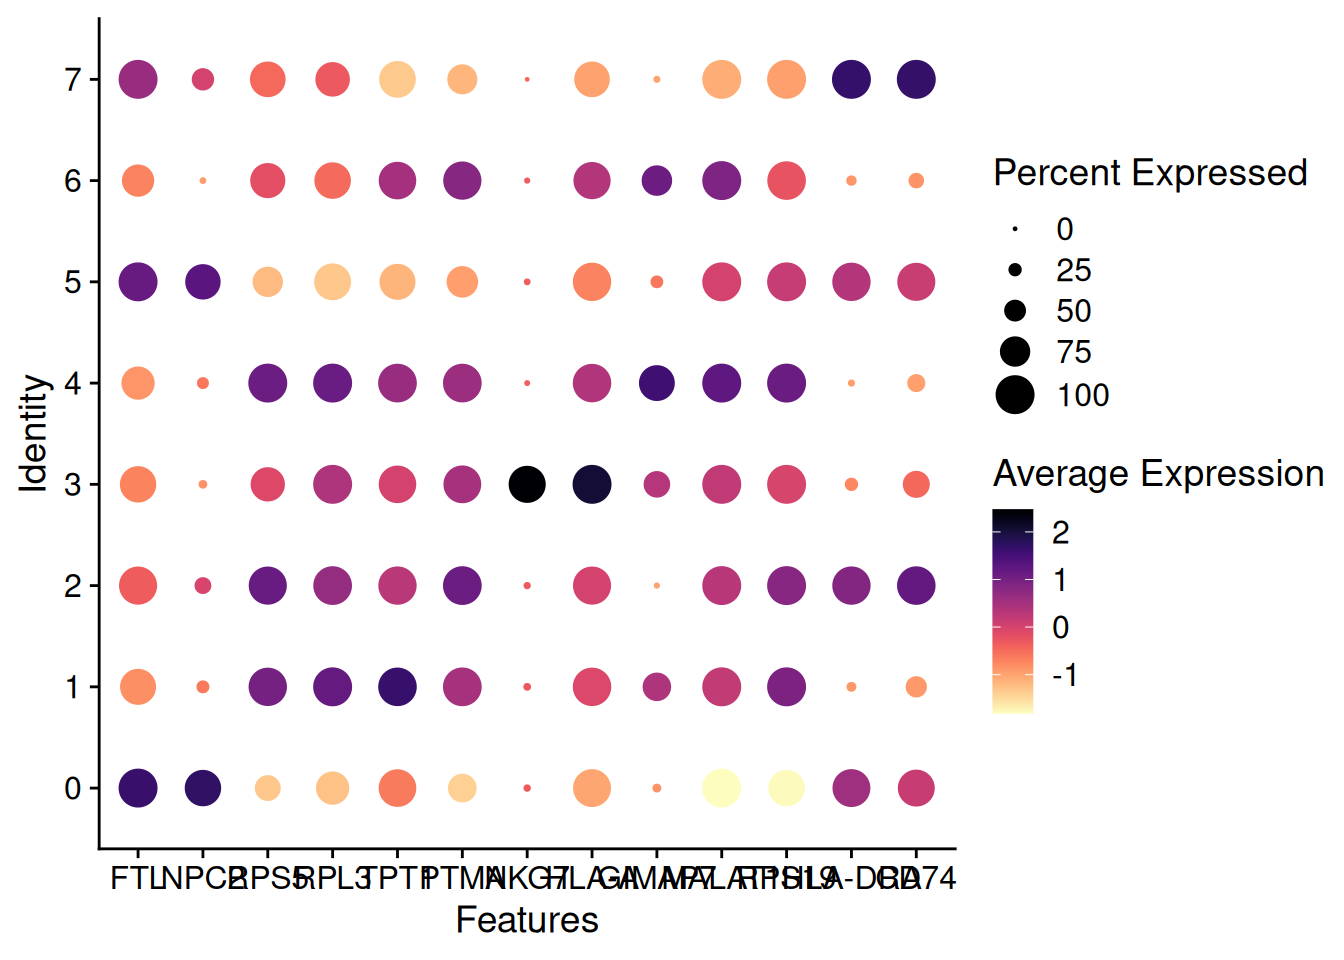
\includegraphics[keepaspectratio]{Intro_files/figure-pdf/unnamed-chunk-57-1.pdf}}

\section{Conclusion}\label{conclusion}

Thanks for joining! If you have questions, you can stop by our Zoom
office hours. For more information, consult the CCV calendar:
https://events.brown.edu/ccv/all




\end{document}
